%!TEX program = xelatex

% Name           : defense.tex
% Author         : Jarrett Keifer (jkeifer0@gmail.com)
% Created on     : 04.09.2014
% Last Edited on : 17.09.2014
% Copyright      : Copyright (c) 2014 by Jarrett Keifer. All rights reserved.
% License        : This file may be distributed and/or modified under the
%                  GNU Public License.
% Description    : Thesis defense slides. Uses a modified version of the
%                  HSRMbeamertheme by Benjamin Weiss.

\documentclass[draft,compress,xcolor={usenames,dvipsnames}]{beamer}

% if handout option for beamer, make 4-up landscape
\mode<handout>{%
  \usepackage{pgfpages}%
  \pgfpagesuselayout{4 on 1}[letterpaper,border shrink=5mm, landscape]}

%--------------------------------------------------------------------------
% Common packages
%--------------------------------------------------------------------------
\usepackage[australian, american]{babel}
\usepackage{datetime}
\setdefaultdate{\dateaustralian}

\newdateformat{noyear}{\THEDAY\ \monthname[\THEMONTH]}
\newdateformat{aagdate}{\THEDAY\ \monthname[\THEMONTH]\ \THEYEAR}

\usepackage{appendixnumberbeamer}

% command to print noyear dates, args {dayno}{monthno}
\newcommand{\datenoyear}[2]{%
  \noyear\formatdate{#1}{#2}{1}%
  \aagdate}
  

\usepackage[overload]{textcase} %provides capitalization protection via \NoCaseChange tag

%\usepackage{tikz}
%\usepackage{tikzscale}
\usepackage{pgf}  % for plots
\usepackage{setspace}

\usepackage[export]{adjustbox}  % for right align of figures

% Colors
%\definecolor{bg}{rgb}{0.95,0.95,0.95} 
\definecolor{light-gray}{gray}{0.85}

% Reference Settings
% *************** Set Biblatex Style and Options ***************

\usepackage{csquotes}
\usepackage[authordate-trad, backend=biber, firstinits=true, maxcitenames=3, isbn=false, doi=false, eprint=false, shorthandfull, sorting=nyt, sortcites=true, ibidtracker=false, abbreviate=true]{biblatex-chicago}
\addbibresource[datatype=bibtex]{thesis.bib}

%Check for page range in postnotes to use a colon not comma
\renewcommand{\postnotedelim}{\iffieldpages{postnote}{\addcolon\space}{\addcomma\space}} 
\DeclareFieldFormat{postnote}{#1} 

%Fix date format in bib -- could be moved to external .lbx file (with comments; change DefineBib... to DeclareBib...)
%%%%\DeclareLanguageMapping{american}{american-dmy}
%%%%
%%%%\begin{filecontents}{american-dmy.lbx}
%%%%\ProvidesFile{american-dmy.lbx}[american localisation with dmydate format for long dates]
%%%%
%%%%\InheritBibliographyExtras{american}
\DefineBibliographyExtras{american}{%
  \protected\def\mkbibdatelong#1#2#3{%
    \iffieldundef{#3}
      {}
      {\stripzeros{\thefield{#3}}%
       \iffieldundef{#2}{}{\nobreakspace}}%
    \iffieldundef{#2}
      {}
      {\mkbibmonth{\thefield{#2}}%
       \iffieldundef{#1}{}{\space}}%
    \iffieldbibstring{#1}{\bibstring{\thefield{#1}}}{\stripzeros{\thefield{#1}}}}%
}
%%%%\InheritBibliographyStrings{american}
%%%%\endinput
%%%%\end{filecontents}

% *************** Make ref links whole ref in text *****************
%%%%\DeclareCiteCommand{\cite}
%%%%  {\usebibmacro{prenote}}
%%%%  {\usebibmacro{citeindex}%
%%%%   \printtext[bibhyperref]{\usebibmacro{cite}}}
%%%%  {\multicitedelim}
%%%%  {\usebibmacro{postnote}}
%%%%
%%%%\DeclareCiteCommand*{\cite}
%%%%  {\usebibmacro{prenote}}
%%%%  {\usebibmacro{citeindex}%
%%%%   \printtext[bibhyperref]{\usebibmacro{citeyear}}}
%%%%  {\multicitedelim}
%%%%  {\usebibmacro{postnote}}
%%%%
%%%%\DeclareCiteCommand{\parencite}[\mkbibparens]
%%%%  {\usebibmacro{prenote}}
%%%%  {\usebibmacro{citeindex}%
%%%%    \printtext[bibhyperref]{\usebibmacro{cite}}}
%%%%  {\multicitedelim}
%%%%  {\usebibmacro{postnote}}
%%%%
%%%%\DeclareCiteCommand*{\parencite}[\mkbibparens]
%%%%  {\usebibmacro{prenote}}
%%%%  {\usebibmacro{citeindex}%
%%%%    \printtext[bibhyperref]{\usebibmacro{citeyear}}}
%%%%  {\multicitedelim}
%%%%  {\usebibmacro{postnote}}
%%%%
%%%%\DeclareCiteCommand{\footcite}[\mkbibfootnote]
%%%%  {\usebibmacro{prenote}}
%%%%  {\usebibmacro{citeindex}%
%%%%  \printtext[bibhyperref]{ \usebibmacro{cite}}}
%%%%  {\multicitedelim}
%%%%  {\usebibmacro{postnote}}
%%%%
%%%%\DeclareCiteCommand{\footcitetext}[\mkbibfootnotetext]
%%%%  {\usebibmacro{prenote}}
%%%%  {\usebibmacro{citeindex}%
%%%%   \printtext[bibhyperref]{\usebibmacro{cite}}}
%%%%  {\multicitedelim}
%%%%  {\usebibmacro{postnote}}
%%%%
%%%%\DeclareCiteCommand{\textcite}
%%%%  {\boolfalse{cbx:parens}}
%%%%  {\usebibmacro{citeindex}%
%%%%   \printtext[bibhyperref]{\usebibmacro{textcite}}}
%%%%  {\ifbool{cbx:parens}
%%%%     {\bibcloseparen\global\boolfalse{cbx:parens}}
%%%%     {}%
%%%%   \multicitedelim}
%%%%  {\usebibmacro{textcite:postnote}}
  
%Set custom strings for url and date labels (available at and last accessed)
\DefineBibliographyStrings{american}{%
  url = {available at},
  urlseen = {last accessed}, 
}
%\DeclareFieldFormat{url}{\bibstring{url}\addcolon\space\url{#1}}  % removed "Available at:" 2014-09-01
\DeclareFieldFormat{urldate}{\mkbibparens{\bibstring{urlseen}\space{#1}}}

% Set url + date appearance in bib (add doi here if needed)
\renewbibmacro*{bib+doi+url}{%
  \usebibmacro{url+urldate}
  }
  

% Abbreviate edited by as eds.
\DeclareFieldFormat{editortype}{\mkbibparens{#1}}
  
%Remove Quotes around titles
\DeclareFieldFormat
  [article,inbook,incollection,inproceedings,patent,thesis,unpublished]
  {title}{#1\isdot}
  
\appto{\bibsetup}{\raggedright} %align left to prevent stretched urls (perhaps remove?)

% /end bib settings


%% Default Packages (Remove if not needed)
\usepackage{graphicx}

% Listingserweiterung
\usepackage{listings}
\lstset{ %
language=[LaTeX]TeX,
basicstyle=\normalsize\ttfamily,
keywordstyle=,
numbers=left,
numberstyle=\tiny\ttfamily,
stepnumber=1,
showspaces=false,
showstringspaces=false,
showtabs=false,
breaklines=true,
frame=tb,
framerule=0.5pt,
tabsize=4,
framexleftmargin=0.5em,
framexrightmargin=0.5em,
xleftmargin=0.5em,
xrightmargin=0.5em
}


%--------------------------------------------------------------------------
% Tables settings
%--------------------------------------------------------------------------
%\usepackage{tabu}
%\usepackage{tabularx,ragged2e}

\usepackage{siunitx}
\sisetup{table-number-alignment = right,
         table-text-alignment = left,
         group-separator={,},
         table-figures-decimal=0,
         group-minimum-digits=4}

% Make table text smaller
\makeatletter
\g@addto@macro{\table}{\footnotesize}
\makeatother

\usepackage{booktabs}
\usepackage{multicol}
\usepackage{multirow}
\usepackage{colortbl}

\newcommand{\alerttab}[2]{\action<#1-|alert@#1>{#2}}% first argument: slide number to appear from, second argument: content of cell

% Custom column types
\usepackage{array}
\newcolumntype{L}[1]{>{\raggedright\let\newline\\\arraybackslash\hspace{0pt}}m{#1}}
\newcolumntype{C}[1]{>{\centering\let\newline\\\arraybackslash\hspace{0pt}}m{#1}}
\newcolumntype{R}[1]{>{\raggedleft\let\newline\\\arraybackslash\hspace{0pt}}m{#1}}

% Caption settings
\usepackage{caption}
\captionsetup{labelformat=empty, skip=0pt,belowskip=0pt}


%--------------------------------------------------------------------------
% Load theme
%--------------------------------------------------------------------------
\usetheme[seriffonts]{hsrm}
\setbeamercovered{transparent=50}

\usepackage{dtklogos} % must be loaded after theme
\usepackage{tikz}
\usetikzlibrary{mindmap,backgrounds}

\usepackage[overload]{textcase}

%--------------------------------------------------------------------------
% General presentation settings
%--------------------------------------------------------------------------
\title{Agricultural Classification of Multi-Temporal MODIS Imagery in Northwest Argentina Using Kansas Crop Phenologies}
\subtitle{}
\date{\formatdate{17}{9}{2014}}
\author{Jarrett Keifer}
\institute{Department of Geography}%Portland State University}

%--------------------------------------------------------------------------
% Notes settings
%--------------------------------------------------------------------------
\setbeameroption{show notes}


% Reset appendix section numbering
\makeatletter
\AtBeginPart{%
  \beamer@tocsectionnumber=0\relax
  \setcounter{section}{0}}
\makeatother


\begin{document}
%--------------------------------------------------------------------------
% Titlepage
%--------------------------------------------------------------------------

\maketitle


%--------------------------------------------------------------------------
% Content
%--------------------------------------------------------------------------

\section*{Questions}

\begin{frame}{Research Questions}

Can I...

\begin{itemize}
  \item<1-> develop a phenological classification toolset?
  \item<2-> extract crop signatures from Kansas data?
  \item<3-> classify an Argentina study area with the Kansas signatures?
\end{itemize}
\end{frame}


%--------------------------------------------------------------------------
% Table of contents
%--------------------------------------------------------------------------
\section*{Outline}
\begin{frame}{Outline}
  % hideallsubsections ist empfehlenswert für längere Präsentationen
  \tableofcontents[hideallsubsections]
\end{frame}


%--------------------------------------------------------------------------
% Content
%--------------------------------------------------------------------------

% BACKGROUND
\section{Background}

\subsection{Deforestation in Argentina}
\begin{frame}{Deforestation in Argentina}
\visible<2->{\begin{itemize}
  \item<2-> 1998 to 2002: 940,000 ha deforested
  \item<3-> \Lightit{Ley de Bosques} \Light{passed in November 2007}
  \begin{itemize}
    \item<4-> Classified red, yellow, and green areas through the \Lightit{Ordenamiento Territorial de los Bosques Nativos} \Light{(Land Management Order for Native Forests, OTBN) passed in 2009}
  \end{itemize}
\end{itemize}}
\end{frame}

\begin{frame}{Deforestation in Argentina}

\begin{table}
  \centering
  \caption{Deforestation in Argentina, 2006 to 2011}
  \label{table:deforestationAR}
  \begin{tabular}{lS[table-unit-alignment=right]
}
  \toprule
  \Book{Time Period} & \Book{Hectares Deforested} \\
  \midrule
  2006 to \Lightit{Ley de Bosques} \Light{(2007)} & 573296 \\
  \Lightit{Ley de Bosques} \Light{to OTBN (2009)} & 473001 \\
  OTBN to 2011 & 459108 \\
  \midrule
  \Book{Total} & 1505405 \\
  \bottomrule
  \end{tabular}
\end{table}
\visible<2>{\begin{itemize}
  \item Deforestation has remained extremely high
  \item Questions the effectiveness of the \Lightit{Ley de Bosques}
  \end{itemize}}
\end{frame}


\subsection{Soy and its Effects}
\begin{frame}{Soy and its Effects}
\begin{itemize}
  \item Argentina's soybean cultivation has continually increased
  \begin{itemize}
    \item 5 million ha in 1993 to 19 million ha in 2011
  \end{itemize}
\end{itemize}
\end{frame}

\begin{frame}{Soy and its Effects}
\begin{itemize}
  \item<1-> Soy production highly mechanized
  \item<2-> Over 99 percent of Argentine soy is genetically modified
  \begin{itemize}
    \item<2-> Resistance to glyphosate = heavy pesticide use
  \end{itemize}
  %\vspace{\baselineskip}
  \item<3-> \alert<4->{Capital requirements cut out small producers}
\end{itemize}
\end{frame}

\begin{frame}{Soy and its Effects}
\begin{itemize}
  \item<1-> Prevailing perception that soy drives deforestation
  \item<2-> Deforestation research has neglected to analyze specific crop cover
\end{itemize}
\end{frame}

\begin{frame}{Goal 1}
\begin{block}{Goal}
  Develop a crop mapping toolset which is efficient\\and economical
\end{block}
\vspace{\baselineskip}
 \visible<2->{Why is this important?
\begin{itemize}
  \item<3-> Better understanding of the dynamics of deforestation
  \item<4-> More effective land management policies
\end{itemize}}
\end{frame}


\subsection{Vegetation Indicies}
\begin{frame}{Vegetation Indicies}
\begin{alertblock}{Problem}
  Must be able to classify crops by type
\end{alertblock}
\vspace{\baselineskip}
 \visible<2->{\begin{itemize}
  \item<2-> A Vegetation Index (VI) can help with crop identification
  \begin{itemize}
    \item<3-> Normalized Difference Vegetation Index (NDVI)
    %\item<3-> Enhanced Vegetation Index (EVI)
  \end{itemize}}
\end{itemize}
\end{frame}

\begin{frame}{Vegetation Indicies}
\begin{block}{NDVI}
  \begin{equation*}
    NDVI = \frac{\rho~_{NIR} - \rho~_{red}}{\rho~_{NIR} + \rho~_{red}}
  \end{equation*}
\end{block}
\vspace{\baselineskip}
 \visible<2->{\begin{itemize}
  \item<2-> is a ratioing index
  \item<3-> minimizes multiplicative noise
  \item<4-> has issues with non-linearity and additive noise
\end{itemize}}
\end{frame}


%\begin{frame}{Vegetation Indicies}
%\begin{block}{EVI}
%  \begin{equation*}
%    EVI = G\frac{\rho~_{NIR} - \rho~_{red}}{\rho~_{NIR} +  C_1\times\rho~_{red} - C_2 \times \rho~_{blue} + L}
%  \end{equation*}
%\end{block}
%\end{frame}
%  
%\begin{frame}{Vegetation Indicies}
%\begin{block}{MODIS EVI}
%  \begin{equation*}
%    EVI = 2.5\frac{\rho~_{NIR} - \rho~_{red}}{\rho~_{NIR} +  6.0\times\rho~_{red} - 7.5 \times \rho~_{blue} + 1.0}
%  \end{equation*}
%\end{block}
%\vspace{\baselineskip} 
%
%\begin{itemize}
%  \item<1-> input bands require atmospheric correction
%  \item<2-> no saturation in high biomass
%\end{itemize}
%\end{frame}

\begin{frame}{Vegetation Indicies}
\begin{alertblock}{Problem}
  Must be able to classify crops by type
\end{alertblock}
\vspace{\baselineskip}
\visible<2->{\begingroup
\setbeamercolor{block title}{bg=hsrmSec2CompDark}
\setbeamercolor{block body}{bg=hsrmSec2Comp}
\begin{block}{Questions}
\begin{itemize}
  \item What if two crops have similar VI values on a single date?
  \item How does one determine a crop's VI values?
\end{itemize}
\end{block}
\endgroup}
\end{frame}

\begin{frame}{Vegetation Indicies}
\begingroup
\setbeamercolor{block title}{bg=hsrmSec2CompDark}
\setbeamercolor{block body}{bg=hsrmSec2Comp}
\begin{block}{Question}
What if two crops have similar VI values on a single date?
\end{block}
\endgroup
\visible<2->{\begin{exampleblock}{Answer}
Use imagery from multiple dates.
\end{exampleblock}}
\end{frame}

\begin{frame}{Time Series Images}
NASA's Moderate Resolution Imaging Spectroradiometer (MODIS) Sensor
\begin{itemize}
  \item<1-> Terra and Aqua satellites
  \item<2-> Each images the Earth once per day
  \item<3-> Composite 16-day NDVI imagery at 250-meter resolution
%  \begin{itemize}
%    \item<3-> Both NDVI and EVI data
%  \end{itemize}
\end{itemize}
\end{frame}


\begin{frame}{Time Series Images}
\begin{columns}[c]
\column{0.4\linewidth}
Time Series Image (TSI)
\begin{itemize}
  \item<+-> Each band is a 16-day VI composite
  \item<+-> Bands are sequential composites
  \item<+-> Contains enough bands to cover an entire growing season
\end{itemize}

\column{0.5\linewidth}
  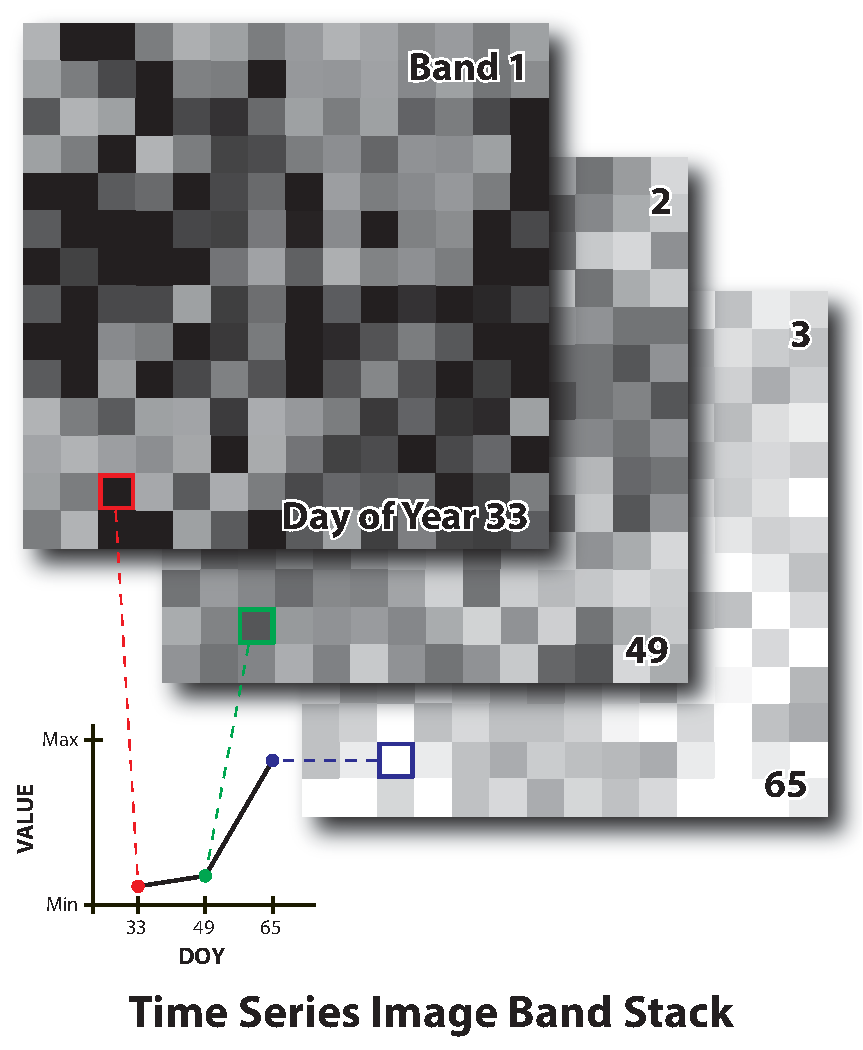
\includegraphics[width=1.1\textwidth,right]{Graphics/tsi_bands_2.pdf}
\end{columns}
\end{frame}

\begin{frame}{Time Series Images}
\begin{block}{Key Points}
\begin{itemize}
  \item A TSI pixel shows VI values over time
  \item Each crop's phenology exhibits a unique temporal signature
\end{itemize}
\end{block}
%\visible<3->{\alert<3>{Sounds like hyperspectral remote sensing, where each pixel shows reflectance over the spectrum, and materials have unique spectral signatures...}}
\end{frame}

\begin{frame}{Crop Temporal Signatures}
\begin{figure}
  \centering
  \includegraphicscopyright[width=0.85\linewidth]{Graphics/wardlowCropSignatures.png}{\autocite[From][]{wardlow2005state-level}}
\end{figure}
\end{frame}

\subsection{Phenological Classification}
\begin{frame}{Phenological Classification}
\begingroup
\setbeamercolor{block title}{bg=hsrmSec2CompDark}
\setbeamercolor{block body}{bg=hsrmSec2Comp}
\begin{block}{Question}
  How does one determine a crop's VI values?
\end{block}
\endgroup
\visible<2->{\begin{exampleblock}{Answer}
  Existing approaches require training sites.
\end{exampleblock}}
%\centering
%\pause\pause~\Book~But what if you don’t have training sites?
\end{frame}

\begin{frame}{Phenological Classification}
\begin{alertblock}{Problem}
  What if you don’t have training sites?
\end{alertblock}
\end{frame}

\begin{frame}{Time Series Images}
\begin{block}{Key Points}
\begin{itemize}
  \item A TSI pixel shows VI values over time
  \item Each crop's phenology exhibits a unique temporal signature
\end{itemize}
\end{block}
\vspace{\baselineskip}
\centering
\visible<2->{\alert{\Medium~Sounds a lot like hyperspectral remote sensing...}}
\end{frame}

\begin{frame}{Time Series Images}
\begingroup
\setbeamercolor{block title}{bg=hsrmSec2CompDark}
\setbeamercolor{block body}{bg=hsrmSec2Comp}
\begin{block}{Idea}
  Could we use a hyperspectal-like method to fit known\\crop signatures to unknown pixels?
\end{block}
\endgroup
\end{frame}

\begin{frame}{Time Series Images}
\begin{figure}
  \centering
  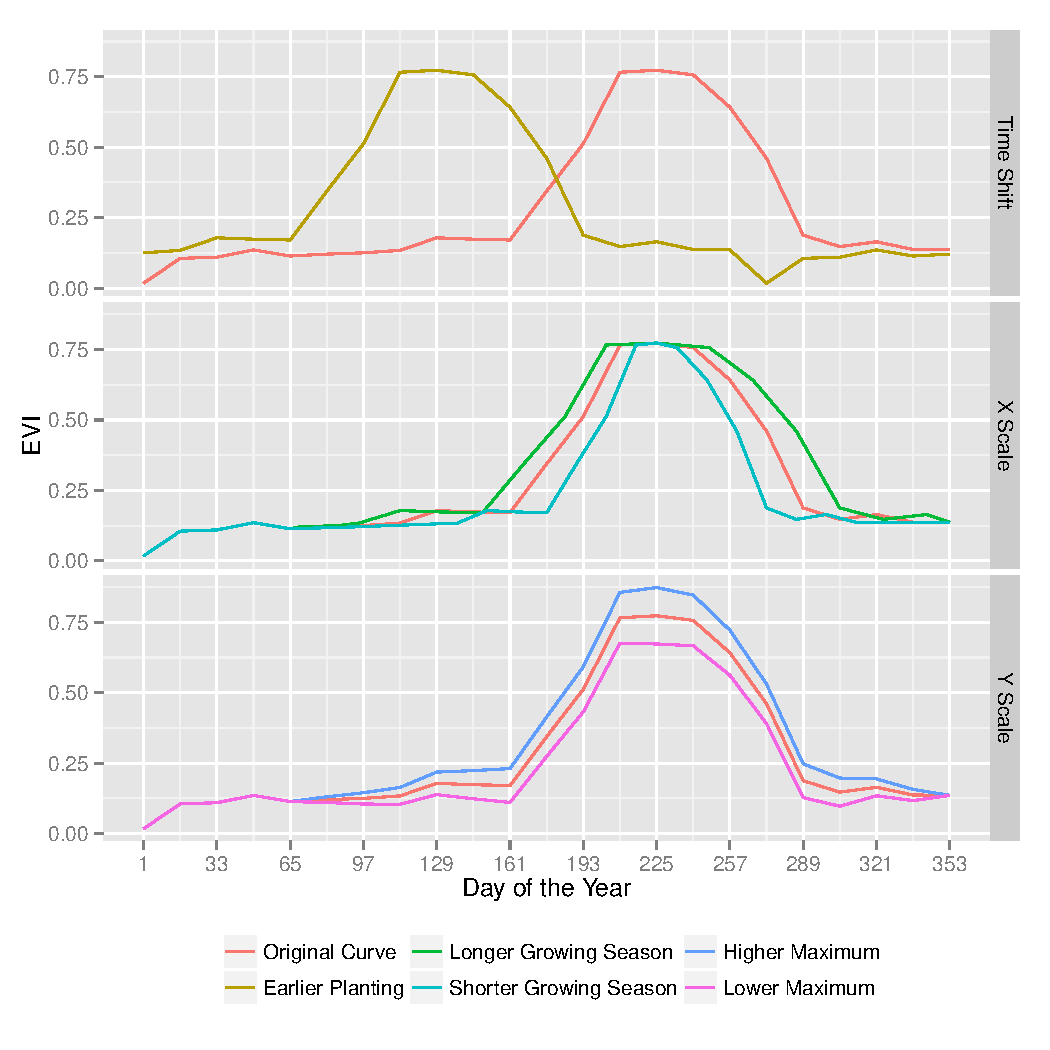
\includegraphics[width=0.7\linewidth]{Graphics/transformations.pdf}
\end{figure}
\end{frame}

\begin{frame}{TSF Method}
Two-Step Filter (TSF) method from \textcite{sakamoto2010a-two-step}
\begin{itemize}
  \item Two steps: (1) wavelet smoothing and (2) curve fitting
  \item Curve fitting can fit reference signature to unknown pixels
\end{itemize}
\end{frame}

\begin{frame}{TSF Method}
\begin{block}{TSF Equation 1}
  \begin{equation*}
    RMSE = \biggl[\frac{1}{365/s}\sum_{x\ =\ j(0),\ j(1)\ldots}^{n}\bigl(f\left(x\right)-g\left(x\right)\bigr)^{2}\biggr]^{\frac{1}{2}}
  \end{equation*}
\end{block}
\vspace{0.5\baselineskip}
where
\begin{itemize}
  \item $n$ is the number of dates in the TSI
  \item $f(x)$ is the temporal signature for a given pixel in a dataset
  \item $x$ is the DOY, as defined by $j(y)$
\end{itemize}
\end{frame}

\begin{frame}{TSF Method}
\begin{block}{TSF Equation 2}
  \begin{equation*}
    g(x) = yscale\times~h\left(xscale\times(x + tshift)\right)
  \end{equation*}
\end{block}
\vspace{0.5\baselineskip}
where
\begin{itemize}
  \item $yscale$ and  $xscale$ are coefficients controlling the vertical and horizontal scaling of a reference signature $h(x)$
  \item $tshift$ is a constant representing the horizontal shift, in days, of $h(x)$
  \item $x$ is the DOY
\end{itemize}
\end{frame}

\begin{frame}{TSF Method}
\begin{figure}
  \centering
  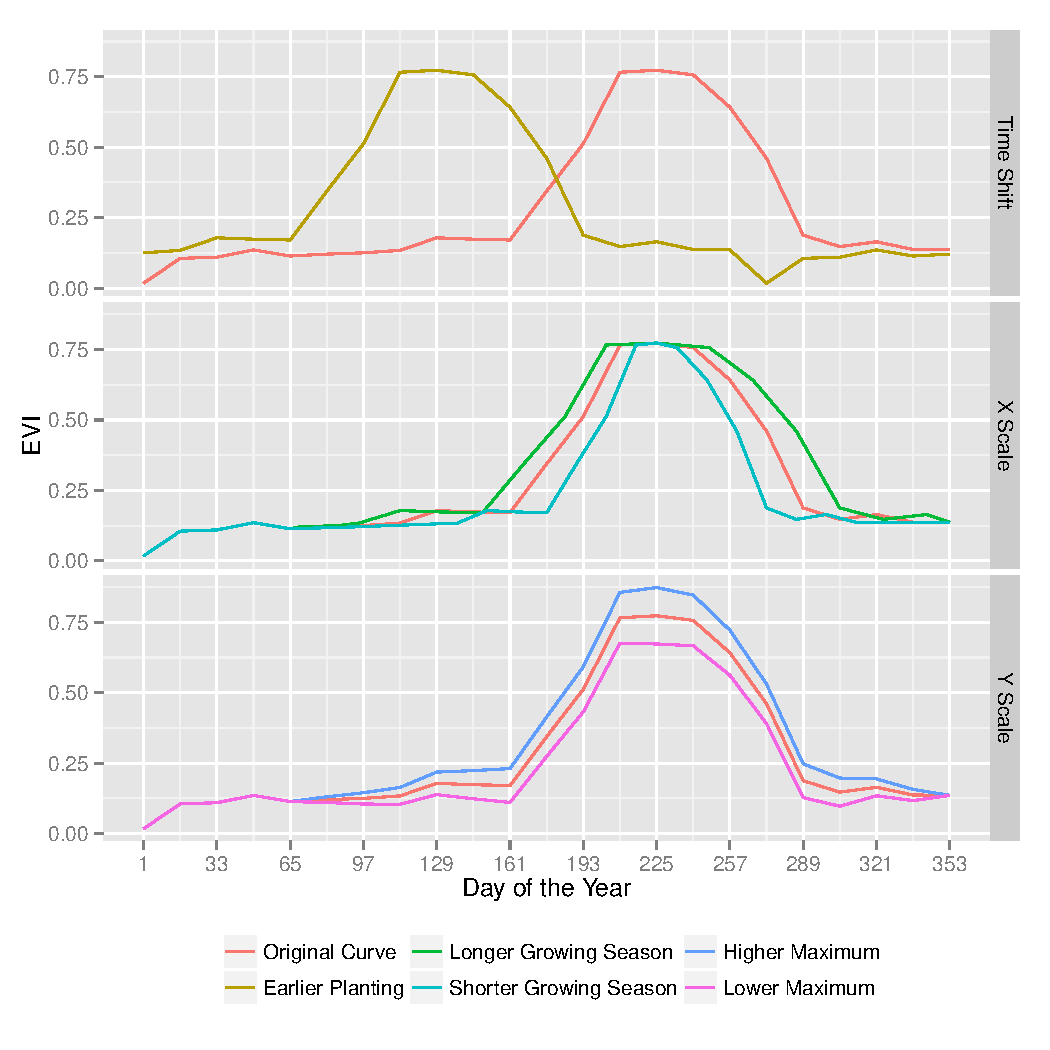
\includegraphics[width=0.7\linewidth]{Graphics/transformations.pdf}
\end{figure}
\end{frame}

\begin{frame}{TSF Method}
\begin{block}{TSF Equation 1}
  \begin{equation*}
    RMSE = \biggl[\frac{1}{365/s}\sum_{x\ =\ j(0),\ j(1)\ldots}^{n}\bigl(f\left(x\right)-g\left(x\right)\bigr)^{2}\biggr]^{\frac{1}{2}}
  \end{equation*}
\end{block}
\vspace{0.5\baselineskip}
Minimizing Equation 1 with appropriate constraints on $yscale$, $xscale$, and $tshift$ will find the fit of a a reference signature to a pixel.

\alert<2>{The signature with the lowest RMSE provides the most probable identification.}
\end{frame}

\begin{frame}{Phenological Classification}
\begin{alertblock}{Problem}
  What if you don’t have training sites?
\end{alertblock}
\visible<2->{\begin{block}{Answer}
  The TSF equations allow the classification of unknown pixels\\using a library of crop signatures.
\end{block}}
\end{frame}


% STUDY AREAS
\section{Study Areas}

\subsection{Kansas}
\begin{frame}{Kansas Study Area}
\begin{columns}[onlytextwidth]
\begin{column}{0.47\textwidth}
  \begin{itemize}
    \item 2012 Kansas top crops:
      \begin{itemize}
        \item Winter wheat
        \item Corn
        \item Soy
      \end{itemize}
    \item Ground truth:\\USDA Cropland Data Layer
  \end{itemize}
\end{column}
\begin{column}{0.53\textwidth}
  \begin{figure}
    \includegraphics[width=1.02\textwidth,right]{Graphics/KSstudysite.pdf}
  \end{figure}
\end{column}
\end{columns}
\end{frame}

\begin{frame}{Kansas Study Area}
\begin{table}
  \centering
  \caption[Kansas Study Site Planting Dates]{\parbox{2.5in}{\centering~Kansas Study Site Planting Dates \scriptsize\autocite[adapted from][]{shroyer1996kansas}}}
  \begin{tabular}{L{.75in} R{1.75in}}
    \toprule
    \Book{Crop} & \Book{Planting Date Range} \\
    \midrule
    Wheat & \datenoyear{25}{9} to \datenoyear{20}{10} \\
    Corn & \datenoyear{1}{4} to \datenoyear{10}{5} \\
    Sorghum & \datenoyear{15}{5} to \datenoyear{20}{6} \\
    Soybeans & \datenoyear{5}{5} to \datenoyear{10}{6} \\
    \bottomrule
  \end{tabular}
\end{table}

\end{frame}



\subsection{Pellegrini}
\begin{frame}{Department of Pellegrini}
  \begin{figure}
    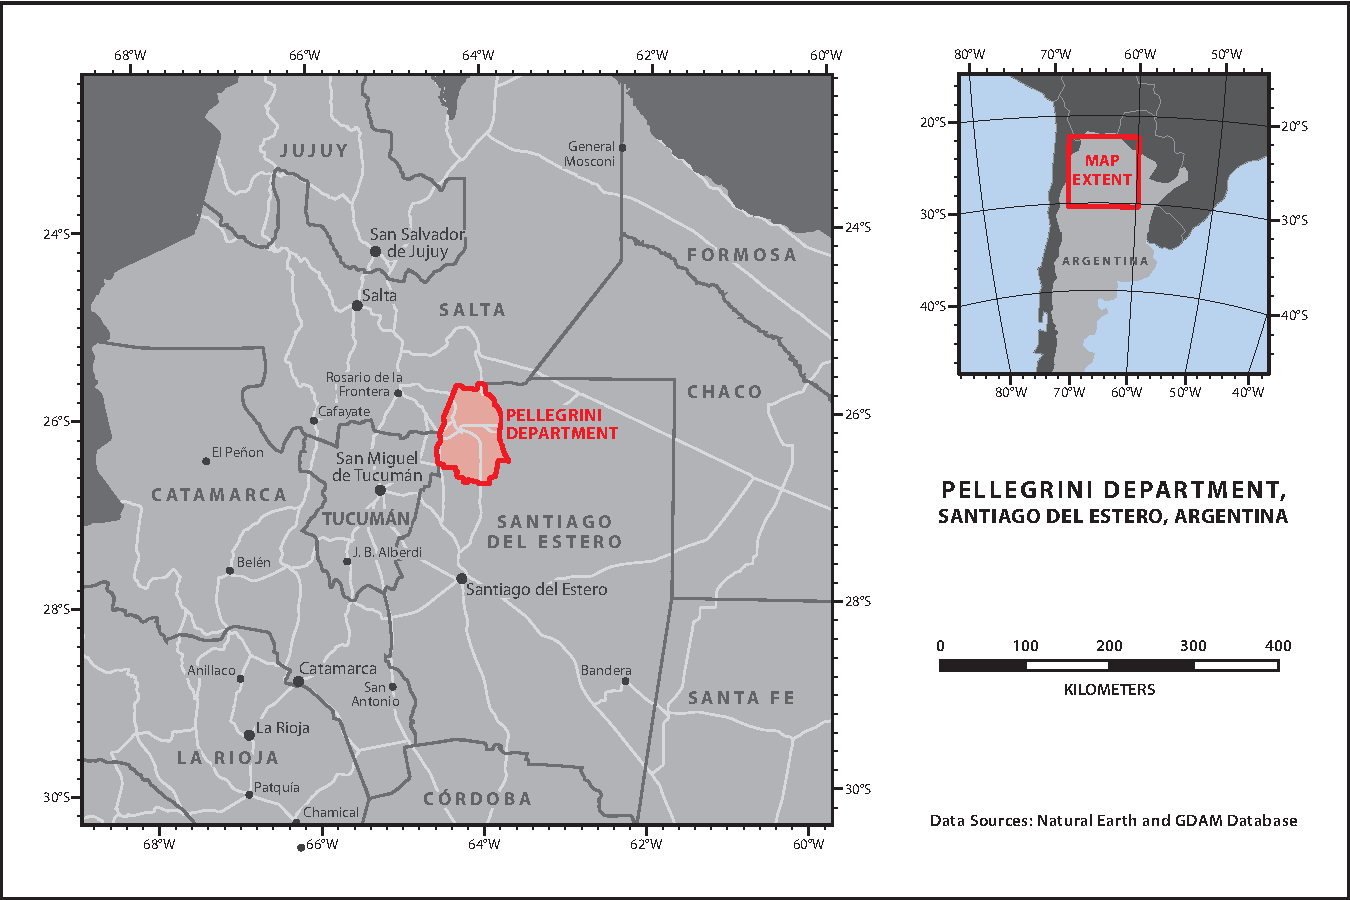
\includegraphics[width=0.97\textwidth]{Graphics/argentinaOverview_landscape.pdf}
  \end{figure}
\end{frame}

\begin{frame}{Department of Pellegrini}
  \begin{figure}
    \includegraphics[width=1.0\textwidth]{Graphics/pellegrini75to14_landscape.pdf}
  \end{figure}
\end{frame}

\begin{frame}{Department of Pellegrini}
\centering

\begin{table}
  \caption{Deforestation in Pellegrini, 2001 to 2011}
  \begin{tabular}{lSS[table-figures-decimal=1]S}  
    \toprule
    \multirow{2}{*}{\Book{Time Period}} & \multirow{2}{*}{\parbox{0.75in}{\raggedleft\Book{Hectares Cleared}}} & \multirow{2}{*}{\parbox{0.75in}{\raggedleft\Book{Percent of Land Area}}} & \multirow{2}{*}{\parbox{0.75in}{\raggedleft\Book{Hectares per Year}}} \\
     & & & \\
    \midrule
    2001 to 2005 & 5968 & 0.9 & 1492 \\
    2006 to 2011 & 75249 & 10.9 & 15050 \\
    \bottomrule
  \end{tabular}
\end{table}
\visible<2>{\vspace{\baselineskip}
\centering
\alert{Annual rate of clearing increased over 1000\%!}}
\end{frame}

\begin{frame}{Department of Pellegrini}
Top crops in Pellegrini, 2001 to 2005
\begin{itemize}
  \item Soy
  \item Corn
  \item Winter Wheat
\end{itemize}
\autocite[From][]{volante2005analisis}
\end{frame}


% DATA AND METHODS
\section{Data and Methods}

\subsection{Datasets}
\begin{frame}{Datasets}
\begin{itemize}
  \item<1-> 250-meter MODIS 16-day composite VI imagery
  \item<2-> 30-meter 2012 USDA Cropland Data Layer
  \item<3-> 30-meter Landsat 8 OLI satellite imagery
  \item<4-> Pellegrini boundary shapefile
\end{itemize}
\end{frame}

\begin{frame}{Datasets}
\begin{itemize}
  \item<1-> 2014 Pellegrini Land Cover vector dataset
\end{itemize}
\end{frame}


\subsection{Pellegrini Data Collection}
\begin{frame}{Pellegrini Data Collection}
\begin{itemize}
  \item<1-> Data collection in Pellegrini \datenoyear{12}{3} to \datenoyear{3}{4}
  \begin{itemize}
    \item<2-> 400 random sample points
    \begin{itemize}
      \item<3-> Direct observation
      \item<3-> Interviews with farmers
      \item<3-> Satellite image interpretation
    \end{itemize}
    \item<4-> Agricultural practices and planting/harvesting dates
  \end{itemize}
\end{itemize}
\end{frame}


\subsection{Data Processing}
\begin{frame}{Processing Workflow}
\begin{enumerate}
  \item Reproject the MODIS composite VIs
  \item Assemble composite VIs into TSIs
  \item Extract crop signatures from the Kansas TSI
  \begin{enumerate}
    \item Identify pure pixels (e.g. non-mixels)
    \item Use the CDL to isolate each crop
    \item Identify phenological groups using k-means clustering
    \item Extract pixel values for each group and average
  \end{enumerate}
  \item Fit the Kansas signatures to the Kansas TSI using the TSF method
  \item Classify the Kansas RMSE rasters and assess accuracy
  \item Fit the Kansas signatures to the Argentina TSI
  \item Classify the Argentina RMSE rasters and assess accuracy
\end{enumerate}
\end{frame}

\begin{frame}{1. Reprojection}
\begin{itemize}
  \item Land Processes Distributed Active Archive Center's (LPDAAC) MODIS Reprojection Tool
\end{itemize}
\end{frame}

\begin{frame}{2. Building the TSI\NoCaseChange{s}}
\begin{itemize}
  \item<1-> Python command line tool (PCLT) to stack composites
  \item<2-> Kansas TSI covered 2012 DOY 97 to 2012 DOY 273
  \item<3-> Argentina TSI covered 2014 DOY -13 to 2014 DOY 161
  \begin{itemize}
    \item<4-> Aqua DOY 105 composite used in place of DOY 113 composite
    \item<4-> DOY 129 interpolated from DOY 105 and DOY 145 composites
  \end{itemize}
\end{itemize}
\end{frame}

\begin{frame}{3. Extract crop signatures}
\begin{enumerate}
  \item[3.1] Identify pure pixels (e.g. non-mixels)
  \begin{itemize}
    % Necessary because mixels do not have pure temporal signatures
    \item<1-> Intersected MODIS pixel grid with vectorized CDL
    \item<2-> Selected all features >= 53,000 m$^2$ in area
  \end{itemize}
\end{enumerate}
\end{frame}

\begin{frame}{3. Extract crop signatures}
\begin{enumerate}
  \item[3.2] Use the CDL to isolate each crop
  \begin{itemize}
    \item<1-> Resampled CDL to MODIS grid by majority
    \item<2-> Isolated the TSI pixels for each crop
      \begin{itemize}
        \item<3-> Corn
        \item<3-> Soy
        \item<3-> Sorghum
      \end{itemize}
  \end{itemize}
\end{enumerate}
\end{frame}

\begin{frame}{3. Extract crop signatures}
\begin{enumerate}
  \item[3.3] Identify phenological groups using k-means clustering
  \begin{itemize}
    \item<1-> ENVI k-means tool
    \item<2-> Three clusters, 1.0\% change threshold, 100 iterations
  \end{itemize}
\end{enumerate}
\end{frame}

\begin{frame}{3. Extract crop signatures}
\begin{enumerate}
  \item[3.3] Extract pixel values for each group and average
  \begin{itemize}
    \item<1-> Pixels from each k-means cluster converted to points
    \item<2-> PCLT to find mean values from points
    \begin{itemize}
      \item<2-> Produces .ref signature files
    \end{itemize}
  \end{itemize}
\end{enumerate}
\visible<3->{\centering~Now we have crop signatures!}
\end{frame}

\begin{frame}{Fitting Signatures}
\begin{enumerate}
  \item[4, 6.] Fit Kansas signatures to {\footnotesize\texttt{<insert study area here>}}\\TSI using TSF method
  \begin{itemize}
    % Kansas to Kansas for testing and verification of signatures and toolset
    \item<2-> Not using the TSF's wavelet filtering
    \item<3-> PCLT to fit reference signatures to a TSI using\\TSF equations
    \begin{itemize}
      \item<3-> Creates a RMSE raster for each signature
      \item<4-> $xscale$ and $yscale$ bounds: 0.6 to 1.4
      \item<5-> $tshift$ bounds: $\pm10$ days Kansas, 120 to 140 days Argentina
    \end{itemize}
  \end{itemize}
\end{enumerate}
\end{frame}

\begin{frame}{Classifying RMSE Rasters}
\begin{enumerate}
  \item[5, 7.] Classify {\footnotesize\texttt{<insert study area here>}} RMSE rasters\\and assess accuracy
  \begin{itemize}
    \item<2-> Signature with lowest RMSE value is best identification
    \item<3-> Not all RMSE values should be considered
    \begin{itemize}
      \item<4-> If all signatures have high RMSE values,\\none are a good match
    \end{itemize}
  \end{itemize}
\end{enumerate}
\visible<5->{\begin{alertblock}{Problem}
  How do we determine which RMSE values to consider?
\end{alertblock}}
\end{frame}

\begin{frame}{Classifying RMSE Rasters}
\begin{alertblock}{Problem}
  How do we determine which RMSE values to consider?
\end{alertblock}
\visible<2->{\begin{block}{Solution\visible<3->{, kind of}}
  Brute force through different threshold combinations, classifying and assessing the accuracy to find the best result.
\end{block}}
\end{frame}

\begin{frame}{Classifying RMSE Rasters}
\begin{enumerate}
  \item[5, 7.] Classify {\footnotesize\texttt{<insert study area here>}} RMSE rasters\\and assess accuracy
  \begin{itemize}
    \item<2-> PCLT to iterate through user-defined range of thresholds
    \item<3-> Classification and accuracy rasters with best combination
  \end{itemize}
\end{enumerate}
\end{frame}


% RESULTS AND DISCUSSION
\section{Results and Discussion}
\begin{frame}{Results}
\begin{itemize}
  \item Summer 2014 Pellegrini ground truth
  \item Pellegrini agricultural practices
  \item Kansas crop signatures
  \item Kansas classification
  \item Pellegrini classification
\end{itemize}
\end{frame}

\subsection{Pellegrini Data}
\begin{frame}{Pellegrini Ground Truth}
\begin{columns}[onlytextwidth]
\begin{column}{0.47\textwidth}
  \begin{itemize}
    \item 378 of 400 sample\\points were identified
    \item Many additional\\fields were collected
  \end{itemize}
\end{column}
\begin{column}{0.53\textwidth}
  \begin{figure}
    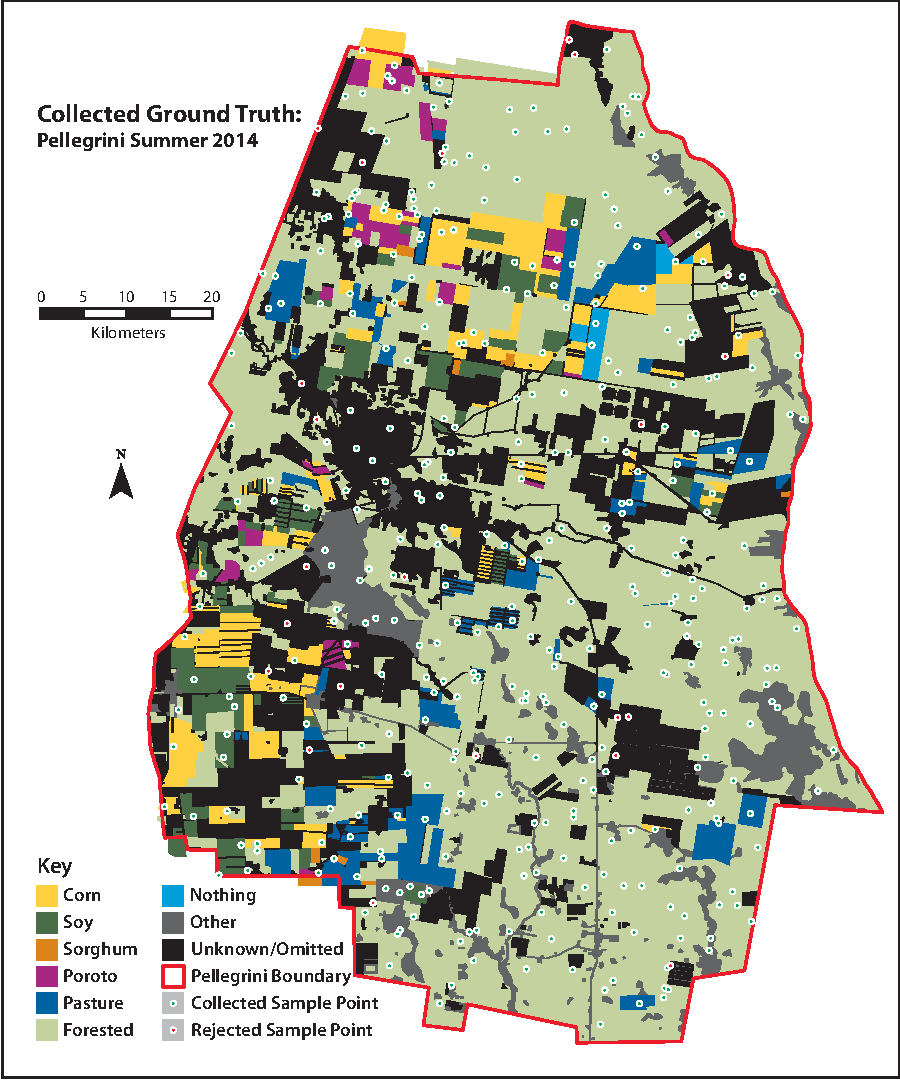
\includegraphics[width=1.0\textwidth]{Graphics/collecteddata.pdf}
  \end{figure}
\end{column}
\end{columns}
\end{frame}

\begin{frame}{Pellegrini Ground Truth}
\begin{table}
  \centering
  \caption{\parbox{4in}{\centering\Book{Summer 2014 Pellegrini Land Cover Classes}}}
  \begin{tabular}{lSS}
    \toprule
    \Book{Cover Type} & \Book{Hectares} & \Book{Sample Points} \\
    \midrule
    Forested & 389541 & 247 \\
    Other & 42229 & 22 \\
    Corn & 41488 & 36 \\
    Pasture & 35057 & 37 \\
    Soy & 27498 & 24 \\
    Poroto & 9539 & 7 \\
    Nothing & 3057 & 3 \\
    Sorghum & 1646 & 2 \\
    \midrule
    Unknown & 92248 & 17 \\
    Omitted & 52052 & 5 \\
    \midrule
    \Book{Total} & 694346 & 400 \\
    \bottomrule
  \end{tabular}
\end{table}
\end{frame}

\begin{frame}{Pellegrini Agriculture}
\begin{table}
  \centering
  \caption{Key Dates for Pellegrini Summer Crops}
  \begin{tabular}{lcc}
    \toprule
    \Book{Crop} & \Book{Ideal Planting Range} & \Book{Harvesting Begins} \\
    \midrule
    Soy & \datenoyear{15}{12} to \datenoyear{15}{1} & \datenoyear{1}{5} \\
    Corn & \datenoyear{15}{1} to \datenoyear{15}{2} & \datenoyear{1}{6} \\
    Sorghum & \datenoyear{15}{1} to \datenoyear{15}{2} & \datenoyear{1}{6} \\
    Poroto & \datenoyear{15}{1} to \datenoyear{20}{2} & \datenoyear{10}{5} \\
    \bottomrule
  \end{tabular}
\end{table}
\end{frame}


\subsection{Kansas Crop Signatures}
\begin{frame}{Kansas Crop Signatures}
\visible<2->{\begin{figure}
  \centering
  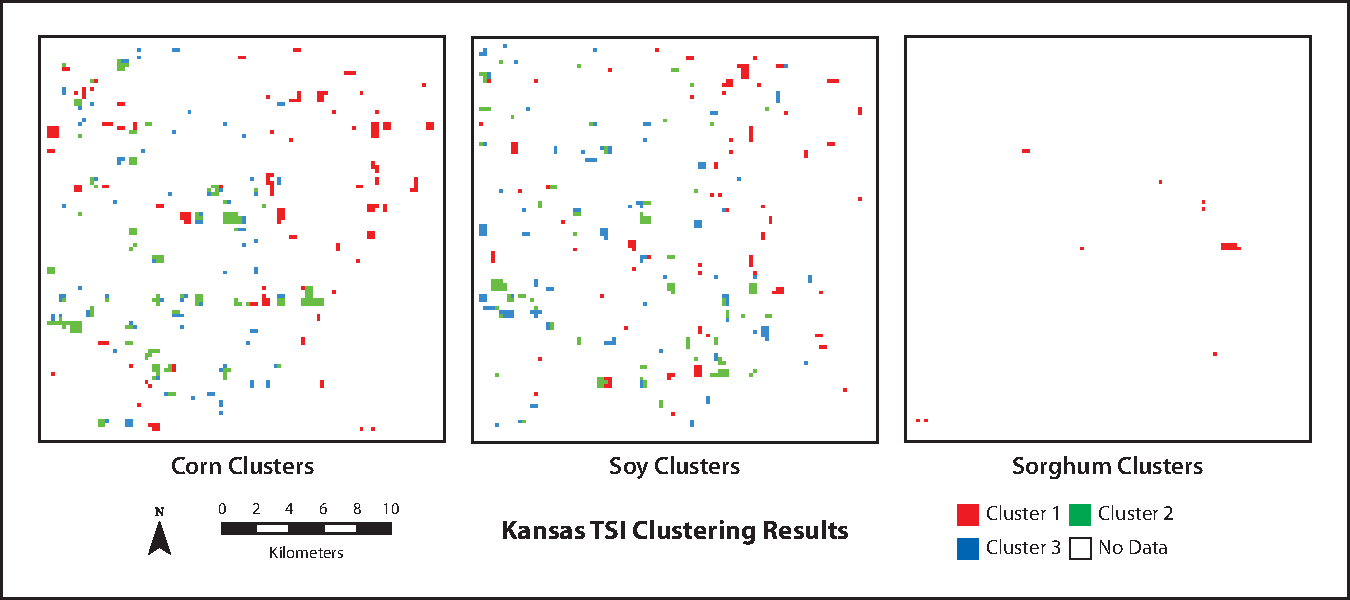
\includegraphics[width=\textwidth]{Graphics/KSclustered.pdf}
\end{figure}}
\end{frame}

\begin{frame}{Kansas Crop Signatures}
\begin{figure}
  \centering
  \resizebox{0.65\textwidth}{!}{%%Signature of ['Soy', 'Corn', 'Sorghum'] from /Users/phoetrymaster/Documents/School/Geography/Thesis/Data/MODIS_KANSAS_2007-2012/reprojected/Summer2012/kmeansTesting_2/KMEANS2_SIGS/ processed with allsigsKS.py.
%% Creator: Matplotlib, PGF backend
%%
%% To include the figure in your LaTeX document, write
%%   \input{<filename>.pgf}
%%
%% Make sure the required packages are loaded in your preamble
%%   \usepackage{pgf}
%%
%% Figures using additional raster images can only be included by \input if
%% they are in the same directory as the main LaTeX file. For loading figures
%% from other directories you can use the `import` package
%%   \usepackage{import}
%% and then include the figures with
%%   \import{<path to file>}{<filename>.pgf}
%%
%% Matplotlib used the following preamble
%%   \usepackage{fontspec}
%%   \setsansfont{Myriad Pro}
%%   \setmonofont{Bitstream Vera Sans Mono}
%%
\begingroup%
\makeatletter%
\begin{pgfpicture}%
\pgfpathrectangle{\pgfpointorigin}{\pgfqpoint{5.149972in}{5.326875in}}%
\pgfusepath{use as bounding box}%
\begin{pgfscope}%
\pgfsetbuttcap%
\pgfsetroundjoin%
\definecolor{currentfill}{rgb}{1.000000,1.000000,1.000000}%
\pgfsetfillcolor{currentfill}%
\pgfsetlinewidth{0.000000pt}%
\definecolor{currentstroke}{rgb}{1.000000,1.000000,1.000000}%
\pgfsetstrokecolor{currentstroke}%
\pgfsetdash{}{0pt}%
\pgfpathmoveto{\pgfqpoint{-0.000000in}{0.000000in}}%
\pgfpathlineto{\pgfqpoint{5.149972in}{0.000000in}}%
\pgfpathlineto{\pgfqpoint{5.149972in}{5.326875in}}%
\pgfpathlineto{\pgfqpoint{-0.000000in}{5.326875in}}%
\pgfpathclose%
\pgfusepath{fill}%
\end{pgfscope}%
\begin{pgfscope}%
\pgfsetbuttcap%
\pgfsetroundjoin%
\definecolor{currentfill}{rgb}{0.898039,0.898039,0.898039}%
\pgfsetfillcolor{currentfill}%
\pgfsetlinewidth{0.000000pt}%
\definecolor{currentstroke}{rgb}{0.000000,0.000000,0.000000}%
\pgfsetstrokecolor{currentstroke}%
\pgfsetstrokeopacity{0.000000}%
\pgfsetdash{}{0pt}%
\pgfpathmoveto{\pgfqpoint{0.593722in}{1.226875in}}%
\pgfpathlineto{\pgfqpoint{5.049972in}{1.226875in}}%
\pgfpathlineto{\pgfqpoint{5.049972in}{5.226875in}}%
\pgfpathlineto{\pgfqpoint{0.593722in}{5.226875in}}%
\pgfpathclose%
\pgfusepath{fill}%
\end{pgfscope}%
\begin{pgfscope}%
\pgfpathrectangle{\pgfqpoint{0.593722in}{1.226875in}}{\pgfqpoint{4.456250in}{4.000000in}} %
\pgfusepath{clip}%
\pgfsetroundcap%
\pgfsetroundjoin%
\pgfsetlinewidth{1.003750pt}%
\definecolor{currentstroke}{rgb}{1.000000,1.000000,1.000000}%
\pgfsetstrokecolor{currentstroke}%
\pgfsetdash{}{0pt}%
\pgfpathmoveto{\pgfqpoint{0.936511in}{1.226875in}}%
\pgfpathlineto{\pgfqpoint{0.936511in}{5.226875in}}%
\pgfusepath{stroke}%
\end{pgfscope}%
\begin{pgfscope}%
\pgfsetbuttcap%
\pgfsetroundjoin%
\definecolor{currentfill}{rgb}{0.5,0.5,0.5}%
\pgfsetfillcolor{currentfill}%
\pgfsetlinewidth{1.003750pt}%
\definecolor{currentstroke}{rgb}{0.5,0.5,0.5}%
\pgfsetstrokecolor{currentstroke}%
\pgfsetdash{}{0pt}%
\pgfsys@defobject{currentmarker}{\pgfqpoint{0.000000in}{-0.055556in}}{\pgfqpoint{0.000000in}{0.000000in}}{%
\pgfpathmoveto{\pgfqpoint{0.000000in}{0.000000in}}%
\pgfpathlineto{\pgfqpoint{0.000000in}{-0.055556in}}%
\pgfusepath{stroke,fill}%
}%
\begin{pgfscope}%
\pgfsys@transformshift{0.936511in}{1.226875in}%
\pgfsys@useobject{currentmarker}{}%
\end{pgfscope}%
\end{pgfscope}%
\begin{pgfscope}%
\definecolor{textcolor}{rgb}{0.5,0.5,0.5}%
\pgfsetstrokecolor{textcolor}%
\pgfsetfillcolor{textcolor}%
\pgftext[x=0.936511in,y=1.115763in,,top]{{\rmfamily\fontsize{10.000000}{12.000000}\selectfont\color{textcolor} 97}}%
\end{pgfscope}%
\begin{pgfscope}%
\pgfpathrectangle{\pgfqpoint{0.593722in}{1.226875in}}{\pgfqpoint{4.456250in}{4.000000in}} %
\pgfusepath{clip}%
\pgfsetroundcap%
\pgfsetroundjoin%
\pgfsetlinewidth{1.003750pt}%
\definecolor{currentstroke}{rgb}{1.000000,1.000000,1.000000}%
\pgfsetstrokecolor{currentstroke}%
\pgfsetdash{}{0pt}%
\pgfpathmoveto{\pgfqpoint{1.622087in}{1.226875in}}%
\pgfpathlineto{\pgfqpoint{1.622087in}{5.226875in}}%
\pgfusepath{stroke}%
\end{pgfscope}%
\begin{pgfscope}%
\pgfsetbuttcap%
\pgfsetroundjoin%
\definecolor{currentfill}{rgb}{0.5,0.5,0.5}%
\pgfsetfillcolor{currentfill}%
\pgfsetlinewidth{1.003750pt}%
\definecolor{currentstroke}{rgb}{0.5,0.5,0.5}%
\pgfsetstrokecolor{currentstroke}%
\pgfsetdash{}{0pt}%
\pgfsys@defobject{currentmarker}{\pgfqpoint{0.000000in}{-0.055556in}}{\pgfqpoint{0.000000in}{0.000000in}}{%
\pgfpathmoveto{\pgfqpoint{0.000000in}{0.000000in}}%
\pgfpathlineto{\pgfqpoint{0.000000in}{-0.055556in}}%
\pgfusepath{stroke,fill}%
}%
\begin{pgfscope}%
\pgfsys@transformshift{1.622087in}{1.226875in}%
\pgfsys@useobject{currentmarker}{}%
\end{pgfscope}%
\end{pgfscope}%
\begin{pgfscope}%
\definecolor{textcolor}{rgb}{0.5,0.5,0.5}%
\pgfsetstrokecolor{textcolor}%
\pgfsetfillcolor{textcolor}%
\pgftext[x=1.622087in,y=1.115763in,,top]{{\rmfamily\fontsize{10.000000}{12.000000}\selectfont\color{textcolor} 129}}%
\end{pgfscope}%
\begin{pgfscope}%
\pgfpathrectangle{\pgfqpoint{0.593722in}{1.226875in}}{\pgfqpoint{4.456250in}{4.000000in}} %
\pgfusepath{clip}%
\pgfsetroundcap%
\pgfsetroundjoin%
\pgfsetlinewidth{1.003750pt}%
\definecolor{currentstroke}{rgb}{1.000000,1.000000,1.000000}%
\pgfsetstrokecolor{currentstroke}%
\pgfsetdash{}{0pt}%
\pgfpathmoveto{\pgfqpoint{2.307664in}{1.226875in}}%
\pgfpathlineto{\pgfqpoint{2.307664in}{5.226875in}}%
\pgfusepath{stroke}%
\end{pgfscope}%
\begin{pgfscope}%
\pgfsetbuttcap%
\pgfsetroundjoin%
\definecolor{currentfill}{rgb}{0.5,0.5,0.5}%
\pgfsetfillcolor{currentfill}%
\pgfsetlinewidth{1.003750pt}%
\definecolor{currentstroke}{rgb}{0.5,0.5,0.5}%
\pgfsetstrokecolor{currentstroke}%
\pgfsetdash{}{0pt}%
\pgfsys@defobject{currentmarker}{\pgfqpoint{0.000000in}{-0.055556in}}{\pgfqpoint{0.000000in}{0.000000in}}{%
\pgfpathmoveto{\pgfqpoint{0.000000in}{0.000000in}}%
\pgfpathlineto{\pgfqpoint{0.000000in}{-0.055556in}}%
\pgfusepath{stroke,fill}%
}%
\begin{pgfscope}%
\pgfsys@transformshift{2.307664in}{1.226875in}%
\pgfsys@useobject{currentmarker}{}%
\end{pgfscope}%
\end{pgfscope}%
\begin{pgfscope}%
\definecolor{textcolor}{rgb}{0.5,0.5,0.5}%
\pgfsetstrokecolor{textcolor}%
\pgfsetfillcolor{textcolor}%
\pgftext[x=2.307664in,y=1.115763in,,top]{{\rmfamily\fontsize{10.000000}{12.000000}\selectfont\color{textcolor} 161}}%
\end{pgfscope}%
\begin{pgfscope}%
\pgfpathrectangle{\pgfqpoint{0.593722in}{1.226875in}}{\pgfqpoint{4.456250in}{4.000000in}} %
\pgfusepath{clip}%
\pgfsetroundcap%
\pgfsetroundjoin%
\pgfsetlinewidth{1.003750pt}%
\definecolor{currentstroke}{rgb}{1.000000,1.000000,1.000000}%
\pgfsetstrokecolor{currentstroke}%
\pgfsetdash{}{0pt}%
\pgfpathmoveto{\pgfqpoint{2.993241in}{1.226875in}}%
\pgfpathlineto{\pgfqpoint{2.993241in}{5.226875in}}%
\pgfusepath{stroke}%
\end{pgfscope}%
\begin{pgfscope}%
\pgfsetbuttcap%
\pgfsetroundjoin%
\definecolor{currentfill}{rgb}{0.5,0.5,0.5}%
\pgfsetfillcolor{currentfill}%
\pgfsetlinewidth{1.003750pt}%
\definecolor{currentstroke}{rgb}{0.5,0.5,0.5}%
\pgfsetstrokecolor{currentstroke}%
\pgfsetdash{}{0pt}%
\pgfsys@defobject{currentmarker}{\pgfqpoint{0.000000in}{-0.055556in}}{\pgfqpoint{0.000000in}{0.000000in}}{%
\pgfpathmoveto{\pgfqpoint{0.000000in}{0.000000in}}%
\pgfpathlineto{\pgfqpoint{0.000000in}{-0.055556in}}%
\pgfusepath{stroke,fill}%
}%
\begin{pgfscope}%
\pgfsys@transformshift{2.993241in}{1.226875in}%
\pgfsys@useobject{currentmarker}{}%
\end{pgfscope}%
\end{pgfscope}%
\begin{pgfscope}%
\definecolor{textcolor}{rgb}{0.5,0.5,0.5}%
\pgfsetstrokecolor{textcolor}%
\pgfsetfillcolor{textcolor}%
\pgftext[x=2.993241in,y=1.115763in,,top]{{\rmfamily\fontsize{10.000000}{12.000000}\selectfont\color{textcolor} 193}}%
\end{pgfscope}%
\begin{pgfscope}%
\pgfpathrectangle{\pgfqpoint{0.593722in}{1.226875in}}{\pgfqpoint{4.456250in}{4.000000in}} %
\pgfusepath{clip}%
\pgfsetroundcap%
\pgfsetroundjoin%
\pgfsetlinewidth{1.003750pt}%
\definecolor{currentstroke}{rgb}{1.000000,1.000000,1.000000}%
\pgfsetstrokecolor{currentstroke}%
\pgfsetdash{}{0pt}%
\pgfpathmoveto{\pgfqpoint{3.678818in}{1.226875in}}%
\pgfpathlineto{\pgfqpoint{3.678818in}{5.226875in}}%
\pgfusepath{stroke}%
\end{pgfscope}%
\begin{pgfscope}%
\pgfsetbuttcap%
\pgfsetroundjoin%
\definecolor{currentfill}{rgb}{0.5,0.5,0.5}%
\pgfsetfillcolor{currentfill}%
\pgfsetlinewidth{1.003750pt}%
\definecolor{currentstroke}{rgb}{0.5,0.5,0.5}%
\pgfsetstrokecolor{currentstroke}%
\pgfsetdash{}{0pt}%
\pgfsys@defobject{currentmarker}{\pgfqpoint{0.000000in}{-0.055556in}}{\pgfqpoint{0.000000in}{0.000000in}}{%
\pgfpathmoveto{\pgfqpoint{0.000000in}{0.000000in}}%
\pgfpathlineto{\pgfqpoint{0.000000in}{-0.055556in}}%
\pgfusepath{stroke,fill}%
}%
\begin{pgfscope}%
\pgfsys@transformshift{3.678818in}{1.226875in}%
\pgfsys@useobject{currentmarker}{}%
\end{pgfscope}%
\end{pgfscope}%
\begin{pgfscope}%
\definecolor{textcolor}{rgb}{0.5,0.5,0.5}%
\pgfsetstrokecolor{textcolor}%
\pgfsetfillcolor{textcolor}%
\pgftext[x=3.678818in,y=1.115763in,,top]{{\rmfamily\fontsize{10.000000}{12.000000}\selectfont\color{textcolor} 225}}%
\end{pgfscope}%
\begin{pgfscope}%
\pgfpathrectangle{\pgfqpoint{0.593722in}{1.226875in}}{\pgfqpoint{4.456250in}{4.000000in}} %
\pgfusepath{clip}%
\pgfsetroundcap%
\pgfsetroundjoin%
\pgfsetlinewidth{1.003750pt}%
\definecolor{currentstroke}{rgb}{1.000000,1.000000,1.000000}%
\pgfsetstrokecolor{currentstroke}%
\pgfsetdash{}{0pt}%
\pgfpathmoveto{\pgfqpoint{4.364395in}{1.226875in}}%
\pgfpathlineto{\pgfqpoint{4.364395in}{5.226875in}}%
\pgfusepath{stroke}%
\end{pgfscope}%
\begin{pgfscope}%
\pgfsetbuttcap%
\pgfsetroundjoin%
\definecolor{currentfill}{rgb}{0.5,0.5,0.5}%
\pgfsetfillcolor{currentfill}%
\pgfsetlinewidth{1.003750pt}%
\definecolor{currentstroke}{rgb}{0.5,0.5,0.5}%
\pgfsetstrokecolor{currentstroke}%
\pgfsetdash{}{0pt}%
\pgfsys@defobject{currentmarker}{\pgfqpoint{0.000000in}{-0.055556in}}{\pgfqpoint{0.000000in}{0.000000in}}{%
\pgfpathmoveto{\pgfqpoint{0.000000in}{0.000000in}}%
\pgfpathlineto{\pgfqpoint{0.000000in}{-0.055556in}}%
\pgfusepath{stroke,fill}%
}%
\begin{pgfscope}%
\pgfsys@transformshift{4.364395in}{1.226875in}%
\pgfsys@useobject{currentmarker}{}%
\end{pgfscope}%
\end{pgfscope}%
\begin{pgfscope}%
\definecolor{textcolor}{rgb}{0.5,0.5,0.5}%
\pgfsetstrokecolor{textcolor}%
\pgfsetfillcolor{textcolor}%
\pgftext[x=4.364395in,y=1.115763in,,top]{{\rmfamily\fontsize{10.000000}{12.000000}\selectfont\color{textcolor} 257}}%
\end{pgfscope}%
\begin{pgfscope}%
\pgfpathrectangle{\pgfqpoint{0.593722in}{1.226875in}}{\pgfqpoint{4.456250in}{4.000000in}} %
\pgfusepath{clip}%
\pgfsetroundcap%
\pgfsetroundjoin%
\pgfsetlinewidth{0.501875pt}%
\definecolor{currentstroke}{rgb}{1.000000,1.000000,1.000000}%
\pgfsetstrokecolor{currentstroke}%
\pgfsetdash{}{0pt}%
\pgfpathmoveto{\pgfqpoint{0.936511in}{1.226875in}}%
\pgfpathlineto{\pgfqpoint{0.936511in}{5.226875in}}%
\pgfusepath{stroke}%
\end{pgfscope}%
\begin{pgfscope}%
\pgfsetbuttcap%
\pgfsetroundjoin%
\definecolor{currentfill}{rgb}{0.5,0.5,0.5}%
\pgfsetfillcolor{currentfill}%
\pgfsetlinewidth{0.501875pt}%
\definecolor{currentstroke}{rgb}{0.5,0.5,0.5}%
\pgfsetstrokecolor{currentstroke}%
\pgfsetdash{}{0pt}%
\pgfsys@defobject{currentmarker}{\pgfqpoint{0.000000in}{0.000000in}}{\pgfqpoint{0.000000in}{0.000000in}}{%
\pgfpathmoveto{\pgfqpoint{0.000000in}{0.000000in}}%
\pgfpathlineto{\pgfqpoint{0.000000in}{0.000000in}}%
\pgfusepath{stroke,fill}%
}%
\begin{pgfscope}%
\pgfsys@transformshift{0.936511in}{1.226875in}%
\pgfsys@useobject{currentmarker}{}%
\end{pgfscope}%
\end{pgfscope}%
\begin{pgfscope}%
\pgfsetbuttcap%
\pgfsetroundjoin%
\definecolor{currentfill}{rgb}{0.5,0.5,0.5}%
\pgfsetfillcolor{currentfill}%
\pgfsetlinewidth{0.501875pt}%
\definecolor{currentstroke}{rgb}{0.5,0.5,0.5}%
\pgfsetstrokecolor{currentstroke}%
\pgfsetdash{}{0pt}%
\pgfsys@defobject{currentmarker}{\pgfqpoint{0.000000in}{0.000000in}}{\pgfqpoint{0.000000in}{0.000000in}}{%
\pgfpathmoveto{\pgfqpoint{0.000000in}{0.000000in}}%
\pgfpathlineto{\pgfqpoint{0.000000in}{0.000000in}}%
\pgfusepath{stroke,fill}%
}%
\begin{pgfscope}%
\pgfsys@transformshift{0.936511in}{5.226875in}%
\pgfsys@useobject{currentmarker}{}%
\end{pgfscope}%
\end{pgfscope}%
\begin{pgfscope}%
\pgfpathrectangle{\pgfqpoint{0.593722in}{1.226875in}}{\pgfqpoint{4.456250in}{4.000000in}} %
\pgfusepath{clip}%
\pgfsetroundcap%
\pgfsetroundjoin%
\pgfsetlinewidth{0.501875pt}%
\definecolor{currentstroke}{rgb}{1.000000,1.000000,1.000000}%
\pgfsetstrokecolor{currentstroke}%
\pgfsetdash{}{0pt}%
\pgfpathmoveto{\pgfqpoint{1.279299in}{1.226875in}}%
\pgfpathlineto{\pgfqpoint{1.279299in}{5.226875in}}%
\pgfusepath{stroke}%
\end{pgfscope}%
\begin{pgfscope}%
\pgfsetbuttcap%
\pgfsetroundjoin%
\definecolor{currentfill}{rgb}{0.5,0.5,0.5}%
\pgfsetfillcolor{currentfill}%
\pgfsetlinewidth{0.501875pt}%
\definecolor{currentstroke}{rgb}{0.5,0.5,0.5}%
\pgfsetstrokecolor{currentstroke}%
\pgfsetdash{}{0pt}%
\pgfsys@defobject{currentmarker}{\pgfqpoint{0.000000in}{0.000000in}}{\pgfqpoint{0.000000in}{0.000000in}}{%
\pgfpathmoveto{\pgfqpoint{0.000000in}{0.000000in}}%
\pgfpathlineto{\pgfqpoint{0.000000in}{0.000000in}}%
\pgfusepath{stroke,fill}%
}%
\begin{pgfscope}%
\pgfsys@transformshift{1.279299in}{1.226875in}%
\pgfsys@useobject{currentmarker}{}%
\end{pgfscope}%
\end{pgfscope}%
\begin{pgfscope}%
\pgfsetbuttcap%
\pgfsetroundjoin%
\definecolor{currentfill}{rgb}{0.5,0.5,0.5}%
\pgfsetfillcolor{currentfill}%
\pgfsetlinewidth{0.501875pt}%
\definecolor{currentstroke}{rgb}{0.5,0.5,0.5}%
\pgfsetstrokecolor{currentstroke}%
\pgfsetdash{}{0pt}%
\pgfsys@defobject{currentmarker}{\pgfqpoint{0.000000in}{0.000000in}}{\pgfqpoint{0.000000in}{0.000000in}}{%
\pgfpathmoveto{\pgfqpoint{0.000000in}{0.000000in}}%
\pgfpathlineto{\pgfqpoint{0.000000in}{0.000000in}}%
\pgfusepath{stroke,fill}%
}%
\begin{pgfscope}%
\pgfsys@transformshift{1.279299in}{5.226875in}%
\pgfsys@useobject{currentmarker}{}%
\end{pgfscope}%
\end{pgfscope}%
\begin{pgfscope}%
\pgfpathrectangle{\pgfqpoint{0.593722in}{1.226875in}}{\pgfqpoint{4.456250in}{4.000000in}} %
\pgfusepath{clip}%
\pgfsetroundcap%
\pgfsetroundjoin%
\pgfsetlinewidth{0.501875pt}%
\definecolor{currentstroke}{rgb}{1.000000,1.000000,1.000000}%
\pgfsetstrokecolor{currentstroke}%
\pgfsetdash{}{0pt}%
\pgfpathmoveto{\pgfqpoint{1.622087in}{1.226875in}}%
\pgfpathlineto{\pgfqpoint{1.622087in}{5.226875in}}%
\pgfusepath{stroke}%
\end{pgfscope}%
\begin{pgfscope}%
\pgfsetbuttcap%
\pgfsetroundjoin%
\definecolor{currentfill}{rgb}{0.5,0.5,0.5}%
\pgfsetfillcolor{currentfill}%
\pgfsetlinewidth{0.501875pt}%
\definecolor{currentstroke}{rgb}{0.5,0.5,0.5}%
\pgfsetstrokecolor{currentstroke}%
\pgfsetdash{}{0pt}%
\pgfsys@defobject{currentmarker}{\pgfqpoint{0.000000in}{0.000000in}}{\pgfqpoint{0.000000in}{0.000000in}}{%
\pgfpathmoveto{\pgfqpoint{0.000000in}{0.000000in}}%
\pgfpathlineto{\pgfqpoint{0.000000in}{0.000000in}}%
\pgfusepath{stroke,fill}%
}%
\begin{pgfscope}%
\pgfsys@transformshift{1.622087in}{1.226875in}%
\pgfsys@useobject{currentmarker}{}%
\end{pgfscope}%
\end{pgfscope}%
\begin{pgfscope}%
\pgfsetbuttcap%
\pgfsetroundjoin%
\definecolor{currentfill}{rgb}{0.5,0.5,0.5}%
\pgfsetfillcolor{currentfill}%
\pgfsetlinewidth{0.501875pt}%
\definecolor{currentstroke}{rgb}{0.5,0.5,0.5}%
\pgfsetstrokecolor{currentstroke}%
\pgfsetdash{}{0pt}%
\pgfsys@defobject{currentmarker}{\pgfqpoint{0.000000in}{0.000000in}}{\pgfqpoint{0.000000in}{0.000000in}}{%
\pgfpathmoveto{\pgfqpoint{0.000000in}{0.000000in}}%
\pgfpathlineto{\pgfqpoint{0.000000in}{0.000000in}}%
\pgfusepath{stroke,fill}%
}%
\begin{pgfscope}%
\pgfsys@transformshift{1.622087in}{5.226875in}%
\pgfsys@useobject{currentmarker}{}%
\end{pgfscope}%
\end{pgfscope}%
\begin{pgfscope}%
\pgfpathrectangle{\pgfqpoint{0.593722in}{1.226875in}}{\pgfqpoint{4.456250in}{4.000000in}} %
\pgfusepath{clip}%
\pgfsetroundcap%
\pgfsetroundjoin%
\pgfsetlinewidth{0.501875pt}%
\definecolor{currentstroke}{rgb}{1.000000,1.000000,1.000000}%
\pgfsetstrokecolor{currentstroke}%
\pgfsetdash{}{0pt}%
\pgfpathmoveto{\pgfqpoint{1.964876in}{1.226875in}}%
\pgfpathlineto{\pgfqpoint{1.964876in}{5.226875in}}%
\pgfusepath{stroke}%
\end{pgfscope}%
\begin{pgfscope}%
\pgfsetbuttcap%
\pgfsetroundjoin%
\definecolor{currentfill}{rgb}{0.5,0.5,0.5}%
\pgfsetfillcolor{currentfill}%
\pgfsetlinewidth{0.501875pt}%
\definecolor{currentstroke}{rgb}{0.5,0.5,0.5}%
\pgfsetstrokecolor{currentstroke}%
\pgfsetdash{}{0pt}%
\pgfsys@defobject{currentmarker}{\pgfqpoint{0.000000in}{0.000000in}}{\pgfqpoint{0.000000in}{0.000000in}}{%
\pgfpathmoveto{\pgfqpoint{0.000000in}{0.000000in}}%
\pgfpathlineto{\pgfqpoint{0.000000in}{0.000000in}}%
\pgfusepath{stroke,fill}%
}%
\begin{pgfscope}%
\pgfsys@transformshift{1.964876in}{1.226875in}%
\pgfsys@useobject{currentmarker}{}%
\end{pgfscope}%
\end{pgfscope}%
\begin{pgfscope}%
\pgfsetbuttcap%
\pgfsetroundjoin%
\definecolor{currentfill}{rgb}{0.5,0.5,0.5}%
\pgfsetfillcolor{currentfill}%
\pgfsetlinewidth{0.501875pt}%
\definecolor{currentstroke}{rgb}{0.5,0.5,0.5}%
\pgfsetstrokecolor{currentstroke}%
\pgfsetdash{}{0pt}%
\pgfsys@defobject{currentmarker}{\pgfqpoint{0.000000in}{0.000000in}}{\pgfqpoint{0.000000in}{0.000000in}}{%
\pgfpathmoveto{\pgfqpoint{0.000000in}{0.000000in}}%
\pgfpathlineto{\pgfqpoint{0.000000in}{0.000000in}}%
\pgfusepath{stroke,fill}%
}%
\begin{pgfscope}%
\pgfsys@transformshift{1.964876in}{5.226875in}%
\pgfsys@useobject{currentmarker}{}%
\end{pgfscope}%
\end{pgfscope}%
\begin{pgfscope}%
\pgfpathrectangle{\pgfqpoint{0.593722in}{1.226875in}}{\pgfqpoint{4.456250in}{4.000000in}} %
\pgfusepath{clip}%
\pgfsetroundcap%
\pgfsetroundjoin%
\pgfsetlinewidth{0.501875pt}%
\definecolor{currentstroke}{rgb}{1.000000,1.000000,1.000000}%
\pgfsetstrokecolor{currentstroke}%
\pgfsetdash{}{0pt}%
\pgfpathmoveto{\pgfqpoint{2.307664in}{1.226875in}}%
\pgfpathlineto{\pgfqpoint{2.307664in}{5.226875in}}%
\pgfusepath{stroke}%
\end{pgfscope}%
\begin{pgfscope}%
\pgfsetbuttcap%
\pgfsetroundjoin%
\definecolor{currentfill}{rgb}{0.5,0.5,0.5}%
\pgfsetfillcolor{currentfill}%
\pgfsetlinewidth{0.501875pt}%
\definecolor{currentstroke}{rgb}{0.5,0.5,0.5}%
\pgfsetstrokecolor{currentstroke}%
\pgfsetdash{}{0pt}%
\pgfsys@defobject{currentmarker}{\pgfqpoint{0.000000in}{0.000000in}}{\pgfqpoint{0.000000in}{0.000000in}}{%
\pgfpathmoveto{\pgfqpoint{0.000000in}{0.000000in}}%
\pgfpathlineto{\pgfqpoint{0.000000in}{0.000000in}}%
\pgfusepath{stroke,fill}%
}%
\begin{pgfscope}%
\pgfsys@transformshift{2.307664in}{1.226875in}%
\pgfsys@useobject{currentmarker}{}%
\end{pgfscope}%
\end{pgfscope}%
\begin{pgfscope}%
\pgfsetbuttcap%
\pgfsetroundjoin%
\definecolor{currentfill}{rgb}{0.5,0.5,0.5}%
\pgfsetfillcolor{currentfill}%
\pgfsetlinewidth{0.501875pt}%
\definecolor{currentstroke}{rgb}{0.5,0.5,0.5}%
\pgfsetstrokecolor{currentstroke}%
\pgfsetdash{}{0pt}%
\pgfsys@defobject{currentmarker}{\pgfqpoint{0.000000in}{0.000000in}}{\pgfqpoint{0.000000in}{0.000000in}}{%
\pgfpathmoveto{\pgfqpoint{0.000000in}{0.000000in}}%
\pgfpathlineto{\pgfqpoint{0.000000in}{0.000000in}}%
\pgfusepath{stroke,fill}%
}%
\begin{pgfscope}%
\pgfsys@transformshift{2.307664in}{5.226875in}%
\pgfsys@useobject{currentmarker}{}%
\end{pgfscope}%
\end{pgfscope}%
\begin{pgfscope}%
\pgfpathrectangle{\pgfqpoint{0.593722in}{1.226875in}}{\pgfqpoint{4.456250in}{4.000000in}} %
\pgfusepath{clip}%
\pgfsetroundcap%
\pgfsetroundjoin%
\pgfsetlinewidth{0.501875pt}%
\definecolor{currentstroke}{rgb}{1.000000,1.000000,1.000000}%
\pgfsetstrokecolor{currentstroke}%
\pgfsetdash{}{0pt}%
\pgfpathmoveto{\pgfqpoint{2.650453in}{1.226875in}}%
\pgfpathlineto{\pgfqpoint{2.650453in}{5.226875in}}%
\pgfusepath{stroke}%
\end{pgfscope}%
\begin{pgfscope}%
\pgfsetbuttcap%
\pgfsetroundjoin%
\definecolor{currentfill}{rgb}{0.5,0.5,0.5}%
\pgfsetfillcolor{currentfill}%
\pgfsetlinewidth{0.501875pt}%
\definecolor{currentstroke}{rgb}{0.5,0.5,0.5}%
\pgfsetstrokecolor{currentstroke}%
\pgfsetdash{}{0pt}%
\pgfsys@defobject{currentmarker}{\pgfqpoint{0.000000in}{0.000000in}}{\pgfqpoint{0.000000in}{0.000000in}}{%
\pgfpathmoveto{\pgfqpoint{0.000000in}{0.000000in}}%
\pgfpathlineto{\pgfqpoint{0.000000in}{0.000000in}}%
\pgfusepath{stroke,fill}%
}%
\begin{pgfscope}%
\pgfsys@transformshift{2.650453in}{1.226875in}%
\pgfsys@useobject{currentmarker}{}%
\end{pgfscope}%
\end{pgfscope}%
\begin{pgfscope}%
\pgfsetbuttcap%
\pgfsetroundjoin%
\definecolor{currentfill}{rgb}{0.5,0.5,0.5}%
\pgfsetfillcolor{currentfill}%
\pgfsetlinewidth{0.501875pt}%
\definecolor{currentstroke}{rgb}{0.5,0.5,0.5}%
\pgfsetstrokecolor{currentstroke}%
\pgfsetdash{}{0pt}%
\pgfsys@defobject{currentmarker}{\pgfqpoint{0.000000in}{0.000000in}}{\pgfqpoint{0.000000in}{0.000000in}}{%
\pgfpathmoveto{\pgfqpoint{0.000000in}{0.000000in}}%
\pgfpathlineto{\pgfqpoint{0.000000in}{0.000000in}}%
\pgfusepath{stroke,fill}%
}%
\begin{pgfscope}%
\pgfsys@transformshift{2.650453in}{5.226875in}%
\pgfsys@useobject{currentmarker}{}%
\end{pgfscope}%
\end{pgfscope}%
\begin{pgfscope}%
\pgfpathrectangle{\pgfqpoint{0.593722in}{1.226875in}}{\pgfqpoint{4.456250in}{4.000000in}} %
\pgfusepath{clip}%
\pgfsetroundcap%
\pgfsetroundjoin%
\pgfsetlinewidth{0.501875pt}%
\definecolor{currentstroke}{rgb}{1.000000,1.000000,1.000000}%
\pgfsetstrokecolor{currentstroke}%
\pgfsetdash{}{0pt}%
\pgfpathmoveto{\pgfqpoint{2.993241in}{1.226875in}}%
\pgfpathlineto{\pgfqpoint{2.993241in}{5.226875in}}%
\pgfusepath{stroke}%
\end{pgfscope}%
\begin{pgfscope}%
\pgfsetbuttcap%
\pgfsetroundjoin%
\definecolor{currentfill}{rgb}{0.5,0.5,0.5}%
\pgfsetfillcolor{currentfill}%
\pgfsetlinewidth{0.501875pt}%
\definecolor{currentstroke}{rgb}{0.5,0.5,0.5}%
\pgfsetstrokecolor{currentstroke}%
\pgfsetdash{}{0pt}%
\pgfsys@defobject{currentmarker}{\pgfqpoint{0.000000in}{0.000000in}}{\pgfqpoint{0.000000in}{0.000000in}}{%
\pgfpathmoveto{\pgfqpoint{0.000000in}{0.000000in}}%
\pgfpathlineto{\pgfqpoint{0.000000in}{0.000000in}}%
\pgfusepath{stroke,fill}%
}%
\begin{pgfscope}%
\pgfsys@transformshift{2.993241in}{1.226875in}%
\pgfsys@useobject{currentmarker}{}%
\end{pgfscope}%
\end{pgfscope}%
\begin{pgfscope}%
\pgfsetbuttcap%
\pgfsetroundjoin%
\definecolor{currentfill}{rgb}{0.5,0.5,0.5}%
\pgfsetfillcolor{currentfill}%
\pgfsetlinewidth{0.501875pt}%
\definecolor{currentstroke}{rgb}{0.5,0.5,0.5}%
\pgfsetstrokecolor{currentstroke}%
\pgfsetdash{}{0pt}%
\pgfsys@defobject{currentmarker}{\pgfqpoint{0.000000in}{0.000000in}}{\pgfqpoint{0.000000in}{0.000000in}}{%
\pgfpathmoveto{\pgfqpoint{0.000000in}{0.000000in}}%
\pgfpathlineto{\pgfqpoint{0.000000in}{0.000000in}}%
\pgfusepath{stroke,fill}%
}%
\begin{pgfscope}%
\pgfsys@transformshift{2.993241in}{5.226875in}%
\pgfsys@useobject{currentmarker}{}%
\end{pgfscope}%
\end{pgfscope}%
\begin{pgfscope}%
\pgfpathrectangle{\pgfqpoint{0.593722in}{1.226875in}}{\pgfqpoint{4.456250in}{4.000000in}} %
\pgfusepath{clip}%
\pgfsetroundcap%
\pgfsetroundjoin%
\pgfsetlinewidth{0.501875pt}%
\definecolor{currentstroke}{rgb}{1.000000,1.000000,1.000000}%
\pgfsetstrokecolor{currentstroke}%
\pgfsetdash{}{0pt}%
\pgfpathmoveto{\pgfqpoint{3.336030in}{1.226875in}}%
\pgfpathlineto{\pgfqpoint{3.336030in}{5.226875in}}%
\pgfusepath{stroke}%
\end{pgfscope}%
\begin{pgfscope}%
\pgfsetbuttcap%
\pgfsetroundjoin%
\definecolor{currentfill}{rgb}{0.5,0.5,0.5}%
\pgfsetfillcolor{currentfill}%
\pgfsetlinewidth{0.501875pt}%
\definecolor{currentstroke}{rgb}{0.5,0.5,0.5}%
\pgfsetstrokecolor{currentstroke}%
\pgfsetdash{}{0pt}%
\pgfsys@defobject{currentmarker}{\pgfqpoint{0.000000in}{0.000000in}}{\pgfqpoint{0.000000in}{0.000000in}}{%
\pgfpathmoveto{\pgfqpoint{0.000000in}{0.000000in}}%
\pgfpathlineto{\pgfqpoint{0.000000in}{0.000000in}}%
\pgfusepath{stroke,fill}%
}%
\begin{pgfscope}%
\pgfsys@transformshift{3.336030in}{1.226875in}%
\pgfsys@useobject{currentmarker}{}%
\end{pgfscope}%
\end{pgfscope}%
\begin{pgfscope}%
\pgfsetbuttcap%
\pgfsetroundjoin%
\definecolor{currentfill}{rgb}{0.5,0.5,0.5}%
\pgfsetfillcolor{currentfill}%
\pgfsetlinewidth{0.501875pt}%
\definecolor{currentstroke}{rgb}{0.5,0.5,0.5}%
\pgfsetstrokecolor{currentstroke}%
\pgfsetdash{}{0pt}%
\pgfsys@defobject{currentmarker}{\pgfqpoint{0.000000in}{0.000000in}}{\pgfqpoint{0.000000in}{0.000000in}}{%
\pgfpathmoveto{\pgfqpoint{0.000000in}{0.000000in}}%
\pgfpathlineto{\pgfqpoint{0.000000in}{0.000000in}}%
\pgfusepath{stroke,fill}%
}%
\begin{pgfscope}%
\pgfsys@transformshift{3.336030in}{5.226875in}%
\pgfsys@useobject{currentmarker}{}%
\end{pgfscope}%
\end{pgfscope}%
\begin{pgfscope}%
\pgfpathrectangle{\pgfqpoint{0.593722in}{1.226875in}}{\pgfqpoint{4.456250in}{4.000000in}} %
\pgfusepath{clip}%
\pgfsetroundcap%
\pgfsetroundjoin%
\pgfsetlinewidth{0.501875pt}%
\definecolor{currentstroke}{rgb}{1.000000,1.000000,1.000000}%
\pgfsetstrokecolor{currentstroke}%
\pgfsetdash{}{0pt}%
\pgfpathmoveto{\pgfqpoint{3.678818in}{1.226875in}}%
\pgfpathlineto{\pgfqpoint{3.678818in}{5.226875in}}%
\pgfusepath{stroke}%
\end{pgfscope}%
\begin{pgfscope}%
\pgfsetbuttcap%
\pgfsetroundjoin%
\definecolor{currentfill}{rgb}{0.5,0.5,0.5}%
\pgfsetfillcolor{currentfill}%
\pgfsetlinewidth{0.501875pt}%
\definecolor{currentstroke}{rgb}{0.5,0.5,0.5}%
\pgfsetstrokecolor{currentstroke}%
\pgfsetdash{}{0pt}%
\pgfsys@defobject{currentmarker}{\pgfqpoint{0.000000in}{0.000000in}}{\pgfqpoint{0.000000in}{0.000000in}}{%
\pgfpathmoveto{\pgfqpoint{0.000000in}{0.000000in}}%
\pgfpathlineto{\pgfqpoint{0.000000in}{0.000000in}}%
\pgfusepath{stroke,fill}%
}%
\begin{pgfscope}%
\pgfsys@transformshift{3.678818in}{1.226875in}%
\pgfsys@useobject{currentmarker}{}%
\end{pgfscope}%
\end{pgfscope}%
\begin{pgfscope}%
\pgfsetbuttcap%
\pgfsetroundjoin%
\definecolor{currentfill}{rgb}{0.5,0.5,0.5}%
\pgfsetfillcolor{currentfill}%
\pgfsetlinewidth{0.501875pt}%
\definecolor{currentstroke}{rgb}{0.5,0.5,0.5}%
\pgfsetstrokecolor{currentstroke}%
\pgfsetdash{}{0pt}%
\pgfsys@defobject{currentmarker}{\pgfqpoint{0.000000in}{0.000000in}}{\pgfqpoint{0.000000in}{0.000000in}}{%
\pgfpathmoveto{\pgfqpoint{0.000000in}{0.000000in}}%
\pgfpathlineto{\pgfqpoint{0.000000in}{0.000000in}}%
\pgfusepath{stroke,fill}%
}%
\begin{pgfscope}%
\pgfsys@transformshift{3.678818in}{5.226875in}%
\pgfsys@useobject{currentmarker}{}%
\end{pgfscope}%
\end{pgfscope}%
\begin{pgfscope}%
\pgfpathrectangle{\pgfqpoint{0.593722in}{1.226875in}}{\pgfqpoint{4.456250in}{4.000000in}} %
\pgfusepath{clip}%
\pgfsetroundcap%
\pgfsetroundjoin%
\pgfsetlinewidth{0.501875pt}%
\definecolor{currentstroke}{rgb}{1.000000,1.000000,1.000000}%
\pgfsetstrokecolor{currentstroke}%
\pgfsetdash{}{0pt}%
\pgfpathmoveto{\pgfqpoint{4.021607in}{1.226875in}}%
\pgfpathlineto{\pgfqpoint{4.021607in}{5.226875in}}%
\pgfusepath{stroke}%
\end{pgfscope}%
\begin{pgfscope}%
\pgfsetbuttcap%
\pgfsetroundjoin%
\definecolor{currentfill}{rgb}{0.5,0.5,0.5}%
\pgfsetfillcolor{currentfill}%
\pgfsetlinewidth{0.501875pt}%
\definecolor{currentstroke}{rgb}{0.5,0.5,0.5}%
\pgfsetstrokecolor{currentstroke}%
\pgfsetdash{}{0pt}%
\pgfsys@defobject{currentmarker}{\pgfqpoint{0.000000in}{0.000000in}}{\pgfqpoint{0.000000in}{0.000000in}}{%
\pgfpathmoveto{\pgfqpoint{0.000000in}{0.000000in}}%
\pgfpathlineto{\pgfqpoint{0.000000in}{0.000000in}}%
\pgfusepath{stroke,fill}%
}%
\begin{pgfscope}%
\pgfsys@transformshift{4.021607in}{1.226875in}%
\pgfsys@useobject{currentmarker}{}%
\end{pgfscope}%
\end{pgfscope}%
\begin{pgfscope}%
\pgfsetbuttcap%
\pgfsetroundjoin%
\definecolor{currentfill}{rgb}{0.5,0.5,0.5}%
\pgfsetfillcolor{currentfill}%
\pgfsetlinewidth{0.501875pt}%
\definecolor{currentstroke}{rgb}{0.5,0.5,0.5}%
\pgfsetstrokecolor{currentstroke}%
\pgfsetdash{}{0pt}%
\pgfsys@defobject{currentmarker}{\pgfqpoint{0.000000in}{0.000000in}}{\pgfqpoint{0.000000in}{0.000000in}}{%
\pgfpathmoveto{\pgfqpoint{0.000000in}{0.000000in}}%
\pgfpathlineto{\pgfqpoint{0.000000in}{0.000000in}}%
\pgfusepath{stroke,fill}%
}%
\begin{pgfscope}%
\pgfsys@transformshift{4.021607in}{5.226875in}%
\pgfsys@useobject{currentmarker}{}%
\end{pgfscope}%
\end{pgfscope}%
\begin{pgfscope}%
\pgfpathrectangle{\pgfqpoint{0.593722in}{1.226875in}}{\pgfqpoint{4.456250in}{4.000000in}} %
\pgfusepath{clip}%
\pgfsetroundcap%
\pgfsetroundjoin%
\pgfsetlinewidth{0.501875pt}%
\definecolor{currentstroke}{rgb}{1.000000,1.000000,1.000000}%
\pgfsetstrokecolor{currentstroke}%
\pgfsetdash{}{0pt}%
\pgfpathmoveto{\pgfqpoint{4.364395in}{1.226875in}}%
\pgfpathlineto{\pgfqpoint{4.364395in}{5.226875in}}%
\pgfusepath{stroke}%
\end{pgfscope}%
\begin{pgfscope}%
\pgfsetbuttcap%
\pgfsetroundjoin%
\definecolor{currentfill}{rgb}{0.5,0.5,0.5}%
\pgfsetfillcolor{currentfill}%
\pgfsetlinewidth{0.501875pt}%
\definecolor{currentstroke}{rgb}{0.5,0.5,0.5}%
\pgfsetstrokecolor{currentstroke}%
\pgfsetdash{}{0pt}%
\pgfsys@defobject{currentmarker}{\pgfqpoint{0.000000in}{0.000000in}}{\pgfqpoint{0.000000in}{0.000000in}}{%
\pgfpathmoveto{\pgfqpoint{0.000000in}{0.000000in}}%
\pgfpathlineto{\pgfqpoint{0.000000in}{0.000000in}}%
\pgfusepath{stroke,fill}%
}%
\begin{pgfscope}%
\pgfsys@transformshift{4.364395in}{1.226875in}%
\pgfsys@useobject{currentmarker}{}%
\end{pgfscope}%
\end{pgfscope}%
\begin{pgfscope}%
\pgfsetbuttcap%
\pgfsetroundjoin%
\definecolor{currentfill}{rgb}{0.5,0.5,0.5}%
\pgfsetfillcolor{currentfill}%
\pgfsetlinewidth{0.501875pt}%
\definecolor{currentstroke}{rgb}{0.5,0.5,0.5}%
\pgfsetstrokecolor{currentstroke}%
\pgfsetdash{}{0pt}%
\pgfsys@defobject{currentmarker}{\pgfqpoint{0.000000in}{0.000000in}}{\pgfqpoint{0.000000in}{0.000000in}}{%
\pgfpathmoveto{\pgfqpoint{0.000000in}{0.000000in}}%
\pgfpathlineto{\pgfqpoint{0.000000in}{0.000000in}}%
\pgfusepath{stroke,fill}%
}%
\begin{pgfscope}%
\pgfsys@transformshift{4.364395in}{5.226875in}%
\pgfsys@useobject{currentmarker}{}%
\end{pgfscope}%
\end{pgfscope}%
\begin{pgfscope}%
\pgfpathrectangle{\pgfqpoint{0.593722in}{1.226875in}}{\pgfqpoint{4.456250in}{4.000000in}} %
\pgfusepath{clip}%
\pgfsetroundcap%
\pgfsetroundjoin%
\pgfsetlinewidth{0.501875pt}%
\definecolor{currentstroke}{rgb}{1.000000,1.000000,1.000000}%
\pgfsetstrokecolor{currentstroke}%
\pgfsetdash{}{0pt}%
\pgfpathmoveto{\pgfqpoint{4.707184in}{1.226875in}}%
\pgfpathlineto{\pgfqpoint{4.707184in}{5.226875in}}%
\pgfusepath{stroke}%
\end{pgfscope}%
\begin{pgfscope}%
\pgfsetbuttcap%
\pgfsetroundjoin%
\definecolor{currentfill}{rgb}{0.5,0.5,0.5}%
\pgfsetfillcolor{currentfill}%
\pgfsetlinewidth{0.501875pt}%
\definecolor{currentstroke}{rgb}{0.5,0.5,0.5}%
\pgfsetstrokecolor{currentstroke}%
\pgfsetdash{}{0pt}%
\pgfsys@defobject{currentmarker}{\pgfqpoint{0.000000in}{0.000000in}}{\pgfqpoint{0.000000in}{0.000000in}}{%
\pgfpathmoveto{\pgfqpoint{0.000000in}{0.000000in}}%
\pgfpathlineto{\pgfqpoint{0.000000in}{0.000000in}}%
\pgfusepath{stroke,fill}%
}%
\begin{pgfscope}%
\pgfsys@transformshift{4.707184in}{1.226875in}%
\pgfsys@useobject{currentmarker}{}%
\end{pgfscope}%
\end{pgfscope}%
\begin{pgfscope}%
\pgfsetbuttcap%
\pgfsetroundjoin%
\definecolor{currentfill}{rgb}{0.5,0.5,0.5}%
\pgfsetfillcolor{currentfill}%
\pgfsetlinewidth{0.501875pt}%
\definecolor{currentstroke}{rgb}{0.5,0.5,0.5}%
\pgfsetstrokecolor{currentstroke}%
\pgfsetdash{}{0pt}%
\pgfsys@defobject{currentmarker}{\pgfqpoint{0.000000in}{0.000000in}}{\pgfqpoint{0.000000in}{0.000000in}}{%
\pgfpathmoveto{\pgfqpoint{0.000000in}{0.000000in}}%
\pgfpathlineto{\pgfqpoint{0.000000in}{0.000000in}}%
\pgfusepath{stroke,fill}%
}%
\begin{pgfscope}%
\pgfsys@transformshift{4.707184in}{5.226875in}%
\pgfsys@useobject{currentmarker}{}%
\end{pgfscope}%
\end{pgfscope}%
\begin{pgfscope}%
\definecolor{textcolor}{rgb}{0.5,0.5,0.5}%
\pgfsetstrokecolor{textcolor}%
\pgfsetfillcolor{textcolor}%
\pgftext[x=2.821847in,y=0.922986in,,top]{{\rmfamily\fontsize{11.000000}{13.200000}\selectfont Day of Year}}%
\end{pgfscope}%
\begin{pgfscope}%
\pgfpathrectangle{\pgfqpoint{0.593722in}{1.226875in}}{\pgfqpoint{4.456250in}{4.000000in}} %
\pgfusepath{clip}%
\pgfsetroundcap%
\pgfsetroundjoin%
\pgfsetlinewidth{1.003750pt}%
\definecolor{currentstroke}{rgb}{1.000000,1.000000,1.000000}%
\pgfsetstrokecolor{currentstroke}%
\pgfsetdash{}{0pt}%
\pgfpathmoveto{\pgfqpoint{0.593722in}{1.322113in}}%
\pgfpathlineto{\pgfqpoint{5.049972in}{1.322113in}}%
\pgfusepath{stroke}%
\end{pgfscope}%
\begin{pgfscope}%
\pgfsetbuttcap%
\pgfsetroundjoin%
\definecolor{currentfill}{rgb}{0.5,0.5,0.5}%
\pgfsetfillcolor{currentfill}%
\pgfsetlinewidth{1.003750pt}%
\definecolor{currentstroke}{rgb}{0.5,0.5,0.5}%
\pgfsetstrokecolor{currentstroke}%
\pgfsetdash{}{0pt}%
\pgfsys@defobject{currentmarker}{\pgfqpoint{-0.055556in}{0.000000in}}{\pgfqpoint{0.000000in}{0.000000in}}{%
\pgfpathmoveto{\pgfqpoint{0.000000in}{0.000000in}}%
\pgfpathlineto{\pgfqpoint{-0.055556in}{0.000000in}}%
\pgfusepath{stroke,fill}%
}%
\begin{pgfscope}%
\pgfsys@transformshift{0.593722in}{1.322113in}%
\pgfsys@useobject{currentmarker}{}%
\end{pgfscope}%
\end{pgfscope}%
\begin{pgfscope}%
\definecolor{textcolor}{rgb}{0.5,0.5,0.5}%
\pgfsetstrokecolor{textcolor}%
\pgfsetfillcolor{textcolor}%
\pgftext[x=0.482611in,y=1.322113in,right,]{{\rmfamily\fontsize{10.000000}{12.000000}\selectfont\color{textcolor} 0.0}}%
\end{pgfscope}%
\begin{pgfscope}%
\pgfpathrectangle{\pgfqpoint{0.593722in}{1.226875in}}{\pgfqpoint{4.456250in}{4.000000in}} %
\pgfusepath{clip}%
\pgfsetroundcap%
\pgfsetroundjoin%
\pgfsetlinewidth{1.003750pt}%
\definecolor{currentstroke}{rgb}{1.000000,1.000000,1.000000}%
\pgfsetstrokecolor{currentstroke}%
\pgfsetdash{}{0pt}%
\pgfpathmoveto{\pgfqpoint{0.593722in}{2.084017in}}%
\pgfpathlineto{\pgfqpoint{5.049972in}{2.084017in}}%
\pgfusepath{stroke}%
\end{pgfscope}%
\begin{pgfscope}%
\pgfsetbuttcap%
\pgfsetroundjoin%
\definecolor{currentfill}{rgb}{0.5,0.5,0.5}%
\pgfsetfillcolor{currentfill}%
\pgfsetlinewidth{1.003750pt}%
\definecolor{currentstroke}{rgb}{0.5,0.5,0.5}%
\pgfsetstrokecolor{currentstroke}%
\pgfsetdash{}{0pt}%
\pgfsys@defobject{currentmarker}{\pgfqpoint{-0.055556in}{0.000000in}}{\pgfqpoint{0.000000in}{0.000000in}}{%
\pgfpathmoveto{\pgfqpoint{0.000000in}{0.000000in}}%
\pgfpathlineto{\pgfqpoint{-0.055556in}{0.000000in}}%
\pgfusepath{stroke,fill}%
}%
\begin{pgfscope}%
\pgfsys@transformshift{0.593722in}{2.084017in}%
\pgfsys@useobject{currentmarker}{}%
\end{pgfscope}%
\end{pgfscope}%
\begin{pgfscope}%
\definecolor{textcolor}{rgb}{0.5,0.5,0.5}%
\pgfsetstrokecolor{textcolor}%
\pgfsetfillcolor{textcolor}%
\pgftext[x=0.482611in,y=2.084017in,right,]{{\rmfamily\fontsize{10.000000}{12.000000}\selectfont\color{textcolor} 0.2}}%
\end{pgfscope}%
\begin{pgfscope}%
\pgfpathrectangle{\pgfqpoint{0.593722in}{1.226875in}}{\pgfqpoint{4.456250in}{4.000000in}} %
\pgfusepath{clip}%
\pgfsetroundcap%
\pgfsetroundjoin%
\pgfsetlinewidth{1.003750pt}%
\definecolor{currentstroke}{rgb}{1.000000,1.000000,1.000000}%
\pgfsetstrokecolor{currentstroke}%
\pgfsetdash{}{0pt}%
\pgfpathmoveto{\pgfqpoint{0.593722in}{2.845922in}}%
\pgfpathlineto{\pgfqpoint{5.049972in}{2.845922in}}%
\pgfusepath{stroke}%
\end{pgfscope}%
\begin{pgfscope}%
\pgfsetbuttcap%
\pgfsetroundjoin%
\definecolor{currentfill}{rgb}{0.5,0.5,0.5}%
\pgfsetfillcolor{currentfill}%
\pgfsetlinewidth{1.003750pt}%
\definecolor{currentstroke}{rgb}{0.5,0.5,0.5}%
\pgfsetstrokecolor{currentstroke}%
\pgfsetdash{}{0pt}%
\pgfsys@defobject{currentmarker}{\pgfqpoint{-0.055556in}{0.000000in}}{\pgfqpoint{0.000000in}{0.000000in}}{%
\pgfpathmoveto{\pgfqpoint{0.000000in}{0.000000in}}%
\pgfpathlineto{\pgfqpoint{-0.055556in}{0.000000in}}%
\pgfusepath{stroke,fill}%
}%
\begin{pgfscope}%
\pgfsys@transformshift{0.593722in}{2.845922in}%
\pgfsys@useobject{currentmarker}{}%
\end{pgfscope}%
\end{pgfscope}%
\begin{pgfscope}%
\definecolor{textcolor}{rgb}{0.5,0.5,0.5}%
\pgfsetstrokecolor{textcolor}%
\pgfsetfillcolor{textcolor}%
\pgftext[x=0.482611in,y=2.845922in,right,]{{\rmfamily\fontsize{10.000000}{12.000000}\selectfont\color{textcolor} 0.4}}%
\end{pgfscope}%
\begin{pgfscope}%
\pgfpathrectangle{\pgfqpoint{0.593722in}{1.226875in}}{\pgfqpoint{4.456250in}{4.000000in}} %
\pgfusepath{clip}%
\pgfsetroundcap%
\pgfsetroundjoin%
\pgfsetlinewidth{1.003750pt}%
\definecolor{currentstroke}{rgb}{1.000000,1.000000,1.000000}%
\pgfsetstrokecolor{currentstroke}%
\pgfsetdash{}{0pt}%
\pgfpathmoveto{\pgfqpoint{0.593722in}{3.607827in}}%
\pgfpathlineto{\pgfqpoint{5.049972in}{3.607827in}}%
\pgfusepath{stroke}%
\end{pgfscope}%
\begin{pgfscope}%
\pgfsetbuttcap%
\pgfsetroundjoin%
\definecolor{currentfill}{rgb}{0.5,0.5,0.5}%
\pgfsetfillcolor{currentfill}%
\pgfsetlinewidth{1.003750pt}%
\definecolor{currentstroke}{rgb}{0.5,0.5,0.5}%
\pgfsetstrokecolor{currentstroke}%
\pgfsetdash{}{0pt}%
\pgfsys@defobject{currentmarker}{\pgfqpoint{-0.055556in}{0.000000in}}{\pgfqpoint{0.000000in}{0.000000in}}{%
\pgfpathmoveto{\pgfqpoint{0.000000in}{0.000000in}}%
\pgfpathlineto{\pgfqpoint{-0.055556in}{0.000000in}}%
\pgfusepath{stroke,fill}%
}%
\begin{pgfscope}%
\pgfsys@transformshift{0.593722in}{3.607827in}%
\pgfsys@useobject{currentmarker}{}%
\end{pgfscope}%
\end{pgfscope}%
\begin{pgfscope}%
\definecolor{textcolor}{rgb}{0.5,0.5,0.5}%
\pgfsetstrokecolor{textcolor}%
\pgfsetfillcolor{textcolor}%
\pgftext[x=0.482611in,y=3.607827in,right,]{{\rmfamily\fontsize{10.000000}{12.000000}\selectfont\color{textcolor} 0.6}}%
\end{pgfscope}%
\begin{pgfscope}%
\pgfpathrectangle{\pgfqpoint{0.593722in}{1.226875in}}{\pgfqpoint{4.456250in}{4.000000in}} %
\pgfusepath{clip}%
\pgfsetroundcap%
\pgfsetroundjoin%
\pgfsetlinewidth{1.003750pt}%
\definecolor{currentstroke}{rgb}{1.000000,1.000000,1.000000}%
\pgfsetstrokecolor{currentstroke}%
\pgfsetdash{}{0pt}%
\pgfpathmoveto{\pgfqpoint{0.593722in}{4.369732in}}%
\pgfpathlineto{\pgfqpoint{5.049972in}{4.369732in}}%
\pgfusepath{stroke}%
\end{pgfscope}%
\begin{pgfscope}%
\pgfsetbuttcap%
\pgfsetroundjoin%
\definecolor{currentfill}{rgb}{0.5,0.5,0.5}%
\pgfsetfillcolor{currentfill}%
\pgfsetlinewidth{1.003750pt}%
\definecolor{currentstroke}{rgb}{0.5,0.5,0.5}%
\pgfsetstrokecolor{currentstroke}%
\pgfsetdash{}{0pt}%
\pgfsys@defobject{currentmarker}{\pgfqpoint{-0.055556in}{0.000000in}}{\pgfqpoint{0.000000in}{0.000000in}}{%
\pgfpathmoveto{\pgfqpoint{0.000000in}{0.000000in}}%
\pgfpathlineto{\pgfqpoint{-0.055556in}{0.000000in}}%
\pgfusepath{stroke,fill}%
}%
\begin{pgfscope}%
\pgfsys@transformshift{0.593722in}{4.369732in}%
\pgfsys@useobject{currentmarker}{}%
\end{pgfscope}%
\end{pgfscope}%
\begin{pgfscope}%
\definecolor{textcolor}{rgb}{0.5,0.5,0.5}%
\pgfsetstrokecolor{textcolor}%
\pgfsetfillcolor{textcolor}%
\pgftext[x=0.482611in,y=4.369732in,right,]{{\rmfamily\fontsize{10.000000}{12.000000}\selectfont\color{textcolor} 0.8}}%
\end{pgfscope}%
\begin{pgfscope}%
\pgfpathrectangle{\pgfqpoint{0.593722in}{1.226875in}}{\pgfqpoint{4.456250in}{4.000000in}} %
\pgfusepath{clip}%
\pgfsetroundcap%
\pgfsetroundjoin%
\pgfsetlinewidth{1.003750pt}%
\definecolor{currentstroke}{rgb}{1.000000,1.000000,1.000000}%
\pgfsetstrokecolor{currentstroke}%
\pgfsetdash{}{0pt}%
\pgfpathmoveto{\pgfqpoint{0.593722in}{5.131636in}}%
\pgfpathlineto{\pgfqpoint{5.049972in}{5.131636in}}%
\pgfusepath{stroke}%
\end{pgfscope}%
\begin{pgfscope}%
\pgfsetbuttcap%
\pgfsetroundjoin%
\definecolor{currentfill}{rgb}{0.5,0.5,0.5}%
\pgfsetfillcolor{currentfill}%
\pgfsetlinewidth{1.003750pt}%
\definecolor{currentstroke}{rgb}{0.5,0.5,0.5}%
\pgfsetstrokecolor{currentstroke}%
\pgfsetdash{}{0pt}%
\pgfsys@defobject{currentmarker}{\pgfqpoint{-0.055556in}{0.000000in}}{\pgfqpoint{0.000000in}{0.000000in}}{%
\pgfpathmoveto{\pgfqpoint{0.000000in}{0.000000in}}%
\pgfpathlineto{\pgfqpoint{-0.055556in}{0.000000in}}%
\pgfusepath{stroke,fill}%
}%
\begin{pgfscope}%
\pgfsys@transformshift{0.593722in}{5.131636in}%
\pgfsys@useobject{currentmarker}{}%
\end{pgfscope}%
\end{pgfscope}%
\begin{pgfscope}%
\definecolor{textcolor}{rgb}{0.5,0.5,0.5}%
\pgfsetstrokecolor{textcolor}%
\pgfsetfillcolor{textcolor}%
\pgftext[x=0.482611in,y=5.131636in,right,]{{\rmfamily\fontsize{10.000000}{12.000000}\selectfont\color{textcolor} 1.0}}%
\end{pgfscope}%
\begin{pgfscope}%
\pgfpathrectangle{\pgfqpoint{0.593722in}{1.226875in}}{\pgfqpoint{4.456250in}{4.000000in}} %
\pgfusepath{clip}%
\pgfsetroundcap%
\pgfsetroundjoin%
\pgfsetlinewidth{0.501875pt}%
\definecolor{currentstroke}{rgb}{1.000000,1.000000,1.000000}%
\pgfsetstrokecolor{currentstroke}%
\pgfsetdash{}{0pt}%
\pgfpathmoveto{\pgfqpoint{0.593722in}{1.322113in}}%
\pgfpathlineto{\pgfqpoint{5.049972in}{1.322113in}}%
\pgfusepath{stroke}%
\end{pgfscope}%
\begin{pgfscope}%
\pgfsetbuttcap%
\pgfsetroundjoin%
\definecolor{currentfill}{rgb}{0.5,0.5,0.5}%
\pgfsetfillcolor{currentfill}%
\pgfsetlinewidth{0.501875pt}%
\definecolor{currentstroke}{rgb}{0.5,0.5,0.5}%
\pgfsetstrokecolor{currentstroke}%
\pgfsetdash{}{0pt}%
\pgfsys@defobject{currentmarker}{\pgfqpoint{0.000000in}{0.000000in}}{\pgfqpoint{0.000000in}{0.000000in}}{%
\pgfpathmoveto{\pgfqpoint{0.000000in}{0.000000in}}%
\pgfpathlineto{\pgfqpoint{0.000000in}{0.000000in}}%
\pgfusepath{stroke,fill}%
}%
\begin{pgfscope}%
\pgfsys@transformshift{0.593722in}{1.322113in}%
\pgfsys@useobject{currentmarker}{}%
\end{pgfscope}%
\end{pgfscope}%
\begin{pgfscope}%
\pgfsetbuttcap%
\pgfsetroundjoin%
\definecolor{currentfill}{rgb}{0.5,0.5,0.5}%
\pgfsetfillcolor{currentfill}%
\pgfsetlinewidth{0.501875pt}%
\definecolor{currentstroke}{rgb}{0.5,0.5,0.5}%
\pgfsetstrokecolor{currentstroke}%
\pgfsetdash{}{0pt}%
\pgfsys@defobject{currentmarker}{\pgfqpoint{0.000000in}{0.000000in}}{\pgfqpoint{0.000000in}{0.000000in}}{%
\pgfpathmoveto{\pgfqpoint{0.000000in}{0.000000in}}%
\pgfpathlineto{\pgfqpoint{0.000000in}{0.000000in}}%
\pgfusepath{stroke,fill}%
}%
\begin{pgfscope}%
\pgfsys@transformshift{5.049972in}{1.322113in}%
\pgfsys@useobject{currentmarker}{}%
\end{pgfscope}%
\end{pgfscope}%
\begin{pgfscope}%
\pgfpathrectangle{\pgfqpoint{0.593722in}{1.226875in}}{\pgfqpoint{4.456250in}{4.000000in}} %
\pgfusepath{clip}%
\pgfsetroundcap%
\pgfsetroundjoin%
\pgfsetlinewidth{0.501875pt}%
\definecolor{currentstroke}{rgb}{1.000000,1.000000,1.000000}%
\pgfsetstrokecolor{currentstroke}%
\pgfsetdash{}{0pt}%
\pgfpathmoveto{\pgfqpoint{0.593722in}{1.703065in}}%
\pgfpathlineto{\pgfqpoint{5.049972in}{1.703065in}}%
\pgfusepath{stroke}%
\end{pgfscope}%
\begin{pgfscope}%
\pgfsetbuttcap%
\pgfsetroundjoin%
\definecolor{currentfill}{rgb}{0.5,0.5,0.5}%
\pgfsetfillcolor{currentfill}%
\pgfsetlinewidth{0.501875pt}%
\definecolor{currentstroke}{rgb}{0.5,0.5,0.5}%
\pgfsetstrokecolor{currentstroke}%
\pgfsetdash{}{0pt}%
\pgfsys@defobject{currentmarker}{\pgfqpoint{0.000000in}{0.000000in}}{\pgfqpoint{0.000000in}{0.000000in}}{%
\pgfpathmoveto{\pgfqpoint{0.000000in}{0.000000in}}%
\pgfpathlineto{\pgfqpoint{0.000000in}{0.000000in}}%
\pgfusepath{stroke,fill}%
}%
\begin{pgfscope}%
\pgfsys@transformshift{0.593722in}{1.703065in}%
\pgfsys@useobject{currentmarker}{}%
\end{pgfscope}%
\end{pgfscope}%
\begin{pgfscope}%
\pgfsetbuttcap%
\pgfsetroundjoin%
\definecolor{currentfill}{rgb}{0.5,0.5,0.5}%
\pgfsetfillcolor{currentfill}%
\pgfsetlinewidth{0.501875pt}%
\definecolor{currentstroke}{rgb}{0.5,0.5,0.5}%
\pgfsetstrokecolor{currentstroke}%
\pgfsetdash{}{0pt}%
\pgfsys@defobject{currentmarker}{\pgfqpoint{0.000000in}{0.000000in}}{\pgfqpoint{0.000000in}{0.000000in}}{%
\pgfpathmoveto{\pgfqpoint{0.000000in}{0.000000in}}%
\pgfpathlineto{\pgfqpoint{0.000000in}{0.000000in}}%
\pgfusepath{stroke,fill}%
}%
\begin{pgfscope}%
\pgfsys@transformshift{5.049972in}{1.703065in}%
\pgfsys@useobject{currentmarker}{}%
\end{pgfscope}%
\end{pgfscope}%
\begin{pgfscope}%
\pgfpathrectangle{\pgfqpoint{0.593722in}{1.226875in}}{\pgfqpoint{4.456250in}{4.000000in}} %
\pgfusepath{clip}%
\pgfsetroundcap%
\pgfsetroundjoin%
\pgfsetlinewidth{0.501875pt}%
\definecolor{currentstroke}{rgb}{1.000000,1.000000,1.000000}%
\pgfsetstrokecolor{currentstroke}%
\pgfsetdash{}{0pt}%
\pgfpathmoveto{\pgfqpoint{0.593722in}{2.084017in}}%
\pgfpathlineto{\pgfqpoint{5.049972in}{2.084017in}}%
\pgfusepath{stroke}%
\end{pgfscope}%
\begin{pgfscope}%
\pgfsetbuttcap%
\pgfsetroundjoin%
\definecolor{currentfill}{rgb}{0.5,0.5,0.5}%
\pgfsetfillcolor{currentfill}%
\pgfsetlinewidth{0.501875pt}%
\definecolor{currentstroke}{rgb}{0.5,0.5,0.5}%
\pgfsetstrokecolor{currentstroke}%
\pgfsetdash{}{0pt}%
\pgfsys@defobject{currentmarker}{\pgfqpoint{0.000000in}{0.000000in}}{\pgfqpoint{0.000000in}{0.000000in}}{%
\pgfpathmoveto{\pgfqpoint{0.000000in}{0.000000in}}%
\pgfpathlineto{\pgfqpoint{0.000000in}{0.000000in}}%
\pgfusepath{stroke,fill}%
}%
\begin{pgfscope}%
\pgfsys@transformshift{0.593722in}{2.084017in}%
\pgfsys@useobject{currentmarker}{}%
\end{pgfscope}%
\end{pgfscope}%
\begin{pgfscope}%
\pgfsetbuttcap%
\pgfsetroundjoin%
\definecolor{currentfill}{rgb}{0.5,0.5,0.5}%
\pgfsetfillcolor{currentfill}%
\pgfsetlinewidth{0.501875pt}%
\definecolor{currentstroke}{rgb}{0.5,0.5,0.5}%
\pgfsetstrokecolor{currentstroke}%
\pgfsetdash{}{0pt}%
\pgfsys@defobject{currentmarker}{\pgfqpoint{0.000000in}{0.000000in}}{\pgfqpoint{0.000000in}{0.000000in}}{%
\pgfpathmoveto{\pgfqpoint{0.000000in}{0.000000in}}%
\pgfpathlineto{\pgfqpoint{0.000000in}{0.000000in}}%
\pgfusepath{stroke,fill}%
}%
\begin{pgfscope}%
\pgfsys@transformshift{5.049972in}{2.084017in}%
\pgfsys@useobject{currentmarker}{}%
\end{pgfscope}%
\end{pgfscope}%
\begin{pgfscope}%
\pgfpathrectangle{\pgfqpoint{0.593722in}{1.226875in}}{\pgfqpoint{4.456250in}{4.000000in}} %
\pgfusepath{clip}%
\pgfsetroundcap%
\pgfsetroundjoin%
\pgfsetlinewidth{0.501875pt}%
\definecolor{currentstroke}{rgb}{1.000000,1.000000,1.000000}%
\pgfsetstrokecolor{currentstroke}%
\pgfsetdash{}{0pt}%
\pgfpathmoveto{\pgfqpoint{0.593722in}{2.464970in}}%
\pgfpathlineto{\pgfqpoint{5.049972in}{2.464970in}}%
\pgfusepath{stroke}%
\end{pgfscope}%
\begin{pgfscope}%
\pgfsetbuttcap%
\pgfsetroundjoin%
\definecolor{currentfill}{rgb}{0.5,0.5,0.5}%
\pgfsetfillcolor{currentfill}%
\pgfsetlinewidth{0.501875pt}%
\definecolor{currentstroke}{rgb}{0.5,0.5,0.5}%
\pgfsetstrokecolor{currentstroke}%
\pgfsetdash{}{0pt}%
\pgfsys@defobject{currentmarker}{\pgfqpoint{0.000000in}{0.000000in}}{\pgfqpoint{0.000000in}{0.000000in}}{%
\pgfpathmoveto{\pgfqpoint{0.000000in}{0.000000in}}%
\pgfpathlineto{\pgfqpoint{0.000000in}{0.000000in}}%
\pgfusepath{stroke,fill}%
}%
\begin{pgfscope}%
\pgfsys@transformshift{0.593722in}{2.464970in}%
\pgfsys@useobject{currentmarker}{}%
\end{pgfscope}%
\end{pgfscope}%
\begin{pgfscope}%
\pgfsetbuttcap%
\pgfsetroundjoin%
\definecolor{currentfill}{rgb}{0.5,0.5,0.5}%
\pgfsetfillcolor{currentfill}%
\pgfsetlinewidth{0.501875pt}%
\definecolor{currentstroke}{rgb}{0.5,0.5,0.5}%
\pgfsetstrokecolor{currentstroke}%
\pgfsetdash{}{0pt}%
\pgfsys@defobject{currentmarker}{\pgfqpoint{0.000000in}{0.000000in}}{\pgfqpoint{0.000000in}{0.000000in}}{%
\pgfpathmoveto{\pgfqpoint{0.000000in}{0.000000in}}%
\pgfpathlineto{\pgfqpoint{0.000000in}{0.000000in}}%
\pgfusepath{stroke,fill}%
}%
\begin{pgfscope}%
\pgfsys@transformshift{5.049972in}{2.464970in}%
\pgfsys@useobject{currentmarker}{}%
\end{pgfscope}%
\end{pgfscope}%
\begin{pgfscope}%
\pgfpathrectangle{\pgfqpoint{0.593722in}{1.226875in}}{\pgfqpoint{4.456250in}{4.000000in}} %
\pgfusepath{clip}%
\pgfsetroundcap%
\pgfsetroundjoin%
\pgfsetlinewidth{0.501875pt}%
\definecolor{currentstroke}{rgb}{1.000000,1.000000,1.000000}%
\pgfsetstrokecolor{currentstroke}%
\pgfsetdash{}{0pt}%
\pgfpathmoveto{\pgfqpoint{0.593722in}{2.845922in}}%
\pgfpathlineto{\pgfqpoint{5.049972in}{2.845922in}}%
\pgfusepath{stroke}%
\end{pgfscope}%
\begin{pgfscope}%
\pgfsetbuttcap%
\pgfsetroundjoin%
\definecolor{currentfill}{rgb}{0.5,0.5,0.5}%
\pgfsetfillcolor{currentfill}%
\pgfsetlinewidth{0.501875pt}%
\definecolor{currentstroke}{rgb}{0.5,0.5,0.5}%
\pgfsetstrokecolor{currentstroke}%
\pgfsetdash{}{0pt}%
\pgfsys@defobject{currentmarker}{\pgfqpoint{0.000000in}{0.000000in}}{\pgfqpoint{0.000000in}{0.000000in}}{%
\pgfpathmoveto{\pgfqpoint{0.000000in}{0.000000in}}%
\pgfpathlineto{\pgfqpoint{0.000000in}{0.000000in}}%
\pgfusepath{stroke,fill}%
}%
\begin{pgfscope}%
\pgfsys@transformshift{0.593722in}{2.845922in}%
\pgfsys@useobject{currentmarker}{}%
\end{pgfscope}%
\end{pgfscope}%
\begin{pgfscope}%
\pgfsetbuttcap%
\pgfsetroundjoin%
\definecolor{currentfill}{rgb}{0.5,0.5,0.5}%
\pgfsetfillcolor{currentfill}%
\pgfsetlinewidth{0.501875pt}%
\definecolor{currentstroke}{rgb}{0.5,0.5,0.5}%
\pgfsetstrokecolor{currentstroke}%
\pgfsetdash{}{0pt}%
\pgfsys@defobject{currentmarker}{\pgfqpoint{0.000000in}{0.000000in}}{\pgfqpoint{0.000000in}{0.000000in}}{%
\pgfpathmoveto{\pgfqpoint{0.000000in}{0.000000in}}%
\pgfpathlineto{\pgfqpoint{0.000000in}{0.000000in}}%
\pgfusepath{stroke,fill}%
}%
\begin{pgfscope}%
\pgfsys@transformshift{5.049972in}{2.845922in}%
\pgfsys@useobject{currentmarker}{}%
\end{pgfscope}%
\end{pgfscope}%
\begin{pgfscope}%
\pgfpathrectangle{\pgfqpoint{0.593722in}{1.226875in}}{\pgfqpoint{4.456250in}{4.000000in}} %
\pgfusepath{clip}%
\pgfsetroundcap%
\pgfsetroundjoin%
\pgfsetlinewidth{0.501875pt}%
\definecolor{currentstroke}{rgb}{1.000000,1.000000,1.000000}%
\pgfsetstrokecolor{currentstroke}%
\pgfsetdash{}{0pt}%
\pgfpathmoveto{\pgfqpoint{0.593722in}{3.226875in}}%
\pgfpathlineto{\pgfqpoint{5.049972in}{3.226875in}}%
\pgfusepath{stroke}%
\end{pgfscope}%
\begin{pgfscope}%
\pgfsetbuttcap%
\pgfsetroundjoin%
\definecolor{currentfill}{rgb}{0.5,0.5,0.5}%
\pgfsetfillcolor{currentfill}%
\pgfsetlinewidth{0.501875pt}%
\definecolor{currentstroke}{rgb}{0.5,0.5,0.5}%
\pgfsetstrokecolor{currentstroke}%
\pgfsetdash{}{0pt}%
\pgfsys@defobject{currentmarker}{\pgfqpoint{0.000000in}{0.000000in}}{\pgfqpoint{0.000000in}{0.000000in}}{%
\pgfpathmoveto{\pgfqpoint{0.000000in}{0.000000in}}%
\pgfpathlineto{\pgfqpoint{0.000000in}{0.000000in}}%
\pgfusepath{stroke,fill}%
}%
\begin{pgfscope}%
\pgfsys@transformshift{0.593722in}{3.226875in}%
\pgfsys@useobject{currentmarker}{}%
\end{pgfscope}%
\end{pgfscope}%
\begin{pgfscope}%
\pgfsetbuttcap%
\pgfsetroundjoin%
\definecolor{currentfill}{rgb}{0.5,0.5,0.5}%
\pgfsetfillcolor{currentfill}%
\pgfsetlinewidth{0.501875pt}%
\definecolor{currentstroke}{rgb}{0.5,0.5,0.5}%
\pgfsetstrokecolor{currentstroke}%
\pgfsetdash{}{0pt}%
\pgfsys@defobject{currentmarker}{\pgfqpoint{0.000000in}{0.000000in}}{\pgfqpoint{0.000000in}{0.000000in}}{%
\pgfpathmoveto{\pgfqpoint{0.000000in}{0.000000in}}%
\pgfpathlineto{\pgfqpoint{0.000000in}{0.000000in}}%
\pgfusepath{stroke,fill}%
}%
\begin{pgfscope}%
\pgfsys@transformshift{5.049972in}{3.226875in}%
\pgfsys@useobject{currentmarker}{}%
\end{pgfscope}%
\end{pgfscope}%
\begin{pgfscope}%
\pgfpathrectangle{\pgfqpoint{0.593722in}{1.226875in}}{\pgfqpoint{4.456250in}{4.000000in}} %
\pgfusepath{clip}%
\pgfsetroundcap%
\pgfsetroundjoin%
\pgfsetlinewidth{0.501875pt}%
\definecolor{currentstroke}{rgb}{1.000000,1.000000,1.000000}%
\pgfsetstrokecolor{currentstroke}%
\pgfsetdash{}{0pt}%
\pgfpathmoveto{\pgfqpoint{0.593722in}{3.607827in}}%
\pgfpathlineto{\pgfqpoint{5.049972in}{3.607827in}}%
\pgfusepath{stroke}%
\end{pgfscope}%
\begin{pgfscope}%
\pgfsetbuttcap%
\pgfsetroundjoin%
\definecolor{currentfill}{rgb}{0.5,0.5,0.5}%
\pgfsetfillcolor{currentfill}%
\pgfsetlinewidth{0.501875pt}%
\definecolor{currentstroke}{rgb}{0.5,0.5,0.5}%
\pgfsetstrokecolor{currentstroke}%
\pgfsetdash{}{0pt}%
\pgfsys@defobject{currentmarker}{\pgfqpoint{0.000000in}{0.000000in}}{\pgfqpoint{0.000000in}{0.000000in}}{%
\pgfpathmoveto{\pgfqpoint{0.000000in}{0.000000in}}%
\pgfpathlineto{\pgfqpoint{0.000000in}{0.000000in}}%
\pgfusepath{stroke,fill}%
}%
\begin{pgfscope}%
\pgfsys@transformshift{0.593722in}{3.607827in}%
\pgfsys@useobject{currentmarker}{}%
\end{pgfscope}%
\end{pgfscope}%
\begin{pgfscope}%
\pgfsetbuttcap%
\pgfsetroundjoin%
\definecolor{currentfill}{rgb}{0.5,0.5,0.5}%
\pgfsetfillcolor{currentfill}%
\pgfsetlinewidth{0.501875pt}%
\definecolor{currentstroke}{rgb}{0.5,0.5,0.5}%
\pgfsetstrokecolor{currentstroke}%
\pgfsetdash{}{0pt}%
\pgfsys@defobject{currentmarker}{\pgfqpoint{0.000000in}{0.000000in}}{\pgfqpoint{0.000000in}{0.000000in}}{%
\pgfpathmoveto{\pgfqpoint{0.000000in}{0.000000in}}%
\pgfpathlineto{\pgfqpoint{0.000000in}{0.000000in}}%
\pgfusepath{stroke,fill}%
}%
\begin{pgfscope}%
\pgfsys@transformshift{5.049972in}{3.607827in}%
\pgfsys@useobject{currentmarker}{}%
\end{pgfscope}%
\end{pgfscope}%
\begin{pgfscope}%
\pgfpathrectangle{\pgfqpoint{0.593722in}{1.226875in}}{\pgfqpoint{4.456250in}{4.000000in}} %
\pgfusepath{clip}%
\pgfsetroundcap%
\pgfsetroundjoin%
\pgfsetlinewidth{0.501875pt}%
\definecolor{currentstroke}{rgb}{1.000000,1.000000,1.000000}%
\pgfsetstrokecolor{currentstroke}%
\pgfsetdash{}{0pt}%
\pgfpathmoveto{\pgfqpoint{0.593722in}{3.988779in}}%
\pgfpathlineto{\pgfqpoint{5.049972in}{3.988779in}}%
\pgfusepath{stroke}%
\end{pgfscope}%
\begin{pgfscope}%
\pgfsetbuttcap%
\pgfsetroundjoin%
\definecolor{currentfill}{rgb}{0.5,0.5,0.5}%
\pgfsetfillcolor{currentfill}%
\pgfsetlinewidth{0.501875pt}%
\definecolor{currentstroke}{rgb}{0.5,0.5,0.5}%
\pgfsetstrokecolor{currentstroke}%
\pgfsetdash{}{0pt}%
\pgfsys@defobject{currentmarker}{\pgfqpoint{0.000000in}{0.000000in}}{\pgfqpoint{0.000000in}{0.000000in}}{%
\pgfpathmoveto{\pgfqpoint{0.000000in}{0.000000in}}%
\pgfpathlineto{\pgfqpoint{0.000000in}{0.000000in}}%
\pgfusepath{stroke,fill}%
}%
\begin{pgfscope}%
\pgfsys@transformshift{0.593722in}{3.988779in}%
\pgfsys@useobject{currentmarker}{}%
\end{pgfscope}%
\end{pgfscope}%
\begin{pgfscope}%
\pgfsetbuttcap%
\pgfsetroundjoin%
\definecolor{currentfill}{rgb}{0.5,0.5,0.5}%
\pgfsetfillcolor{currentfill}%
\pgfsetlinewidth{0.501875pt}%
\definecolor{currentstroke}{rgb}{0.5,0.5,0.5}%
\pgfsetstrokecolor{currentstroke}%
\pgfsetdash{}{0pt}%
\pgfsys@defobject{currentmarker}{\pgfqpoint{0.000000in}{0.000000in}}{\pgfqpoint{0.000000in}{0.000000in}}{%
\pgfpathmoveto{\pgfqpoint{0.000000in}{0.000000in}}%
\pgfpathlineto{\pgfqpoint{0.000000in}{0.000000in}}%
\pgfusepath{stroke,fill}%
}%
\begin{pgfscope}%
\pgfsys@transformshift{5.049972in}{3.988779in}%
\pgfsys@useobject{currentmarker}{}%
\end{pgfscope}%
\end{pgfscope}%
\begin{pgfscope}%
\pgfpathrectangle{\pgfqpoint{0.593722in}{1.226875in}}{\pgfqpoint{4.456250in}{4.000000in}} %
\pgfusepath{clip}%
\pgfsetroundcap%
\pgfsetroundjoin%
\pgfsetlinewidth{0.501875pt}%
\definecolor{currentstroke}{rgb}{1.000000,1.000000,1.000000}%
\pgfsetstrokecolor{currentstroke}%
\pgfsetdash{}{0pt}%
\pgfpathmoveto{\pgfqpoint{0.593722in}{4.369732in}}%
\pgfpathlineto{\pgfqpoint{5.049972in}{4.369732in}}%
\pgfusepath{stroke}%
\end{pgfscope}%
\begin{pgfscope}%
\pgfsetbuttcap%
\pgfsetroundjoin%
\definecolor{currentfill}{rgb}{0.5,0.5,0.5}%
\pgfsetfillcolor{currentfill}%
\pgfsetlinewidth{0.501875pt}%
\definecolor{currentstroke}{rgb}{0.5,0.5,0.5}%
\pgfsetstrokecolor{currentstroke}%
\pgfsetdash{}{0pt}%
\pgfsys@defobject{currentmarker}{\pgfqpoint{0.000000in}{0.000000in}}{\pgfqpoint{0.000000in}{0.000000in}}{%
\pgfpathmoveto{\pgfqpoint{0.000000in}{0.000000in}}%
\pgfpathlineto{\pgfqpoint{0.000000in}{0.000000in}}%
\pgfusepath{stroke,fill}%
}%
\begin{pgfscope}%
\pgfsys@transformshift{0.593722in}{4.369732in}%
\pgfsys@useobject{currentmarker}{}%
\end{pgfscope}%
\end{pgfscope}%
\begin{pgfscope}%
\pgfsetbuttcap%
\pgfsetroundjoin%
\definecolor{currentfill}{rgb}{0.5,0.5,0.5}%
\pgfsetfillcolor{currentfill}%
\pgfsetlinewidth{0.501875pt}%
\definecolor{currentstroke}{rgb}{0.5,0.5,0.5}%
\pgfsetstrokecolor{currentstroke}%
\pgfsetdash{}{0pt}%
\pgfsys@defobject{currentmarker}{\pgfqpoint{0.000000in}{0.000000in}}{\pgfqpoint{0.000000in}{0.000000in}}{%
\pgfpathmoveto{\pgfqpoint{0.000000in}{0.000000in}}%
\pgfpathlineto{\pgfqpoint{0.000000in}{0.000000in}}%
\pgfusepath{stroke,fill}%
}%
\begin{pgfscope}%
\pgfsys@transformshift{5.049972in}{4.369732in}%
\pgfsys@useobject{currentmarker}{}%
\end{pgfscope}%
\end{pgfscope}%
\begin{pgfscope}%
\pgfpathrectangle{\pgfqpoint{0.593722in}{1.226875in}}{\pgfqpoint{4.456250in}{4.000000in}} %
\pgfusepath{clip}%
\pgfsetroundcap%
\pgfsetroundjoin%
\pgfsetlinewidth{0.501875pt}%
\definecolor{currentstroke}{rgb}{1.000000,1.000000,1.000000}%
\pgfsetstrokecolor{currentstroke}%
\pgfsetdash{}{0pt}%
\pgfpathmoveto{\pgfqpoint{0.593722in}{4.750684in}}%
\pgfpathlineto{\pgfqpoint{5.049972in}{4.750684in}}%
\pgfusepath{stroke}%
\end{pgfscope}%
\begin{pgfscope}%
\pgfsetbuttcap%
\pgfsetroundjoin%
\definecolor{currentfill}{rgb}{0.5,0.5,0.5}%
\pgfsetfillcolor{currentfill}%
\pgfsetlinewidth{0.501875pt}%
\definecolor{currentstroke}{rgb}{0.5,0.5,0.5}%
\pgfsetstrokecolor{currentstroke}%
\pgfsetdash{}{0pt}%
\pgfsys@defobject{currentmarker}{\pgfqpoint{0.000000in}{0.000000in}}{\pgfqpoint{0.000000in}{0.000000in}}{%
\pgfpathmoveto{\pgfqpoint{0.000000in}{0.000000in}}%
\pgfpathlineto{\pgfqpoint{0.000000in}{0.000000in}}%
\pgfusepath{stroke,fill}%
}%
\begin{pgfscope}%
\pgfsys@transformshift{0.593722in}{4.750684in}%
\pgfsys@useobject{currentmarker}{}%
\end{pgfscope}%
\end{pgfscope}%
\begin{pgfscope}%
\pgfsetbuttcap%
\pgfsetroundjoin%
\definecolor{currentfill}{rgb}{0.5,0.5,0.5}%
\pgfsetfillcolor{currentfill}%
\pgfsetlinewidth{0.501875pt}%
\definecolor{currentstroke}{rgb}{0.5,0.5,0.5}%
\pgfsetstrokecolor{currentstroke}%
\pgfsetdash{}{0pt}%
\pgfsys@defobject{currentmarker}{\pgfqpoint{0.000000in}{0.000000in}}{\pgfqpoint{0.000000in}{0.000000in}}{%
\pgfpathmoveto{\pgfqpoint{0.000000in}{0.000000in}}%
\pgfpathlineto{\pgfqpoint{0.000000in}{0.000000in}}%
\pgfusepath{stroke,fill}%
}%
\begin{pgfscope}%
\pgfsys@transformshift{5.049972in}{4.750684in}%
\pgfsys@useobject{currentmarker}{}%
\end{pgfscope}%
\end{pgfscope}%
\begin{pgfscope}%
\pgfpathrectangle{\pgfqpoint{0.593722in}{1.226875in}}{\pgfqpoint{4.456250in}{4.000000in}} %
\pgfusepath{clip}%
\pgfsetroundcap%
\pgfsetroundjoin%
\pgfsetlinewidth{0.501875pt}%
\definecolor{currentstroke}{rgb}{1.000000,1.000000,1.000000}%
\pgfsetstrokecolor{currentstroke}%
\pgfsetdash{}{0pt}%
\pgfpathmoveto{\pgfqpoint{0.593722in}{5.131636in}}%
\pgfpathlineto{\pgfqpoint{5.049972in}{5.131636in}}%
\pgfusepath{stroke}%
\end{pgfscope}%
\begin{pgfscope}%
\pgfsetbuttcap%
\pgfsetroundjoin%
\definecolor{currentfill}{rgb}{0.5,0.5,0.5}%
\pgfsetfillcolor{currentfill}%
\pgfsetlinewidth{0.501875pt}%
\definecolor{currentstroke}{rgb}{0.5,0.5,0.5}%
\pgfsetstrokecolor{currentstroke}%
\pgfsetdash{}{0pt}%
\pgfsys@defobject{currentmarker}{\pgfqpoint{0.000000in}{0.000000in}}{\pgfqpoint{0.000000in}{0.000000in}}{%
\pgfpathmoveto{\pgfqpoint{0.000000in}{0.000000in}}%
\pgfpathlineto{\pgfqpoint{0.000000in}{0.000000in}}%
\pgfusepath{stroke,fill}%
}%
\begin{pgfscope}%
\pgfsys@transformshift{0.593722in}{5.131636in}%
\pgfsys@useobject{currentmarker}{}%
\end{pgfscope}%
\end{pgfscope}%
\begin{pgfscope}%
\pgfsetbuttcap%
\pgfsetroundjoin%
\definecolor{currentfill}{rgb}{0.5,0.5,0.5}%
\pgfsetfillcolor{currentfill}%
\pgfsetlinewidth{0.501875pt}%
\definecolor{currentstroke}{rgb}{0.5,0.5,0.5}%
\pgfsetstrokecolor{currentstroke}%
\pgfsetdash{}{0pt}%
\pgfsys@defobject{currentmarker}{\pgfqpoint{0.000000in}{0.000000in}}{\pgfqpoint{0.000000in}{0.000000in}}{%
\pgfpathmoveto{\pgfqpoint{0.000000in}{0.000000in}}%
\pgfpathlineto{\pgfqpoint{0.000000in}{0.000000in}}%
\pgfusepath{stroke,fill}%
}%
\begin{pgfscope}%
\pgfsys@transformshift{5.049972in}{5.131636in}%
\pgfsys@useobject{currentmarker}{}%
\end{pgfscope}%
\end{pgfscope}%
\begin{pgfscope}%
\definecolor{textcolor}{rgb}{0.5,0.5,0.5}%
\pgfsetstrokecolor{textcolor}%
\pgfsetfillcolor{textcolor}%
\pgftext[x=0.235667in,y=3.226875in,,bottom,rotate=90.000000]{{\rmfamily\fontsize{11.000000}{13.200000}\selectfont NDVI}}%
\end{pgfscope}%
\begin{pgfscope}%
\pgfpathrectangle{\pgfqpoint{0.593722in}{1.226875in}}{\pgfqpoint{4.456250in}{4.000000in}} %
\pgfusepath{clip}%
\pgfsetroundcap%
\pgfsetroundjoin%
\pgfsetlinewidth{2.007500pt}%
\definecolor{currentstroke}{rgb}{1.000000,1.000000,1.000000}%
\pgfsetstrokecolor{currentstroke}%
\pgfsetdash{}{0pt}%
\pgfpathmoveto{\pgfqpoint{0.936511in}{3.409000in}}%
\pgfpathlineto{\pgfqpoint{1.279299in}{3.182013in}}%
\pgfpathlineto{\pgfqpoint{1.622087in}{2.851903in}}%
\pgfpathlineto{\pgfqpoint{1.964876in}{2.667360in}}%
\pgfpathlineto{\pgfqpoint{2.307664in}{3.217010in}}%
\pgfpathlineto{\pgfqpoint{2.650453in}{3.395323in}}%
\pgfpathlineto{\pgfqpoint{2.993241in}{3.439207in}}%
\pgfpathlineto{\pgfqpoint{3.336030in}{3.240171in}}%
\pgfpathlineto{\pgfqpoint{3.678818in}{3.338666in}}%
\pgfpathlineto{\pgfqpoint{4.021607in}{3.599527in}}%
\pgfpathlineto{\pgfqpoint{4.364395in}{3.462071in}}%
\pgfpathlineto{\pgfqpoint{4.707184in}{3.147279in}}%
\pgfusepath{stroke}%
\end{pgfscope}%
\begin{pgfscope}%
\pgfpathrectangle{\pgfqpoint{0.593722in}{1.226875in}}{\pgfqpoint{4.456250in}{4.000000in}} %
\pgfusepath{clip}%
\pgfsetroundcap%
\pgfsetroundjoin%
\pgfsetlinewidth{1.254687pt}%
\definecolor{currentstroke}{rgb}{0.000000,0.750000,0.750000}%
\pgfsetstrokecolor{currentstroke}%
\pgfsetdash{}{0pt}%
\pgfpathmoveto{\pgfqpoint{0.936511in}{3.409000in}}%
\pgfpathlineto{\pgfqpoint{1.279299in}{3.182013in}}%
\pgfpathlineto{\pgfqpoint{1.622087in}{2.851903in}}%
\pgfpathlineto{\pgfqpoint{1.964876in}{2.667360in}}%
\pgfpathlineto{\pgfqpoint{2.307664in}{3.217010in}}%
\pgfpathlineto{\pgfqpoint{2.650453in}{3.395323in}}%
\pgfpathlineto{\pgfqpoint{2.993241in}{3.439207in}}%
\pgfpathlineto{\pgfqpoint{3.336030in}{3.240171in}}%
\pgfpathlineto{\pgfqpoint{3.678818in}{3.338666in}}%
\pgfpathlineto{\pgfqpoint{4.021607in}{3.599527in}}%
\pgfpathlineto{\pgfqpoint{4.364395in}{3.462071in}}%
\pgfpathlineto{\pgfqpoint{4.707184in}{3.147279in}}%
\pgfusepath{stroke}%
\end{pgfscope}%
\begin{pgfscope}%
\pgfpathrectangle{\pgfqpoint{0.593722in}{1.226875in}}{\pgfqpoint{4.456250in}{4.000000in}} %
\pgfusepath{clip}%
\pgfsetroundcap%
\pgfsetroundjoin%
\pgfsetlinewidth{2.007500pt}%
\definecolor{currentstroke}{rgb}{1.000000,1.000000,1.000000}%
\pgfsetstrokecolor{currentstroke}%
\pgfsetdash{{6.000000pt}{6.000000pt}}{0.000000pt}%
\pgfpathmoveto{\pgfqpoint{0.936511in}{2.823880in}}%
\pgfpathlineto{\pgfqpoint{1.279299in}{2.675200in}}%
\pgfpathlineto{\pgfqpoint{1.622087in}{2.623650in}}%
\pgfpathlineto{\pgfqpoint{1.964876in}{2.910398in}}%
\pgfpathlineto{\pgfqpoint{2.307664in}{3.667925in}}%
\pgfpathlineto{\pgfqpoint{2.650453in}{4.018520in}}%
\pgfpathlineto{\pgfqpoint{2.993241in}{4.392359in}}%
\pgfpathlineto{\pgfqpoint{3.336030in}{4.327545in}}%
\pgfpathlineto{\pgfqpoint{3.678818in}{4.310737in}}%
\pgfpathlineto{\pgfqpoint{4.021607in}{4.210444in}}%
\pgfpathlineto{\pgfqpoint{4.364395in}{3.580336in}}%
\pgfpathlineto{\pgfqpoint{4.707184in}{2.830533in}}%
\pgfusepath{stroke}%
\end{pgfscope}%
\begin{pgfscope}%
\pgfpathrectangle{\pgfqpoint{0.593722in}{1.226875in}}{\pgfqpoint{4.456250in}{4.000000in}} %
\pgfusepath{clip}%
\pgfsetroundcap%
\pgfsetroundjoin%
\pgfsetlinewidth{1.254687pt}%
\definecolor{currentstroke}{rgb}{0.000000,0.750000,0.750000}%
\pgfsetstrokecolor{currentstroke}%
\pgfsetdash{{6.000000pt}{6.000000pt}}{0.000000pt}%
\pgfpathmoveto{\pgfqpoint{0.936511in}{2.823880in}}%
\pgfpathlineto{\pgfqpoint{1.279299in}{2.675200in}}%
\pgfpathlineto{\pgfqpoint{1.622087in}{2.623650in}}%
\pgfpathlineto{\pgfqpoint{1.964876in}{2.910398in}}%
\pgfpathlineto{\pgfqpoint{2.307664in}{3.667925in}}%
\pgfpathlineto{\pgfqpoint{2.650453in}{4.018520in}}%
\pgfpathlineto{\pgfqpoint{2.993241in}{4.392359in}}%
\pgfpathlineto{\pgfqpoint{3.336030in}{4.327545in}}%
\pgfpathlineto{\pgfqpoint{3.678818in}{4.310737in}}%
\pgfpathlineto{\pgfqpoint{4.021607in}{4.210444in}}%
\pgfpathlineto{\pgfqpoint{4.364395in}{3.580336in}}%
\pgfpathlineto{\pgfqpoint{4.707184in}{2.830533in}}%
\pgfusepath{stroke}%
\end{pgfscope}%
\begin{pgfscope}%
\pgfpathrectangle{\pgfqpoint{0.593722in}{1.226875in}}{\pgfqpoint{4.456250in}{4.000000in}} %
\pgfusepath{clip}%
\pgfsetroundcap%
\pgfsetroundjoin%
\pgfsetlinewidth{2.007500pt}%
\definecolor{currentstroke}{rgb}{1.000000,1.000000,1.000000}%
\pgfsetstrokecolor{currentstroke}%
\pgfsetdash{{1.000000pt}{3.000000pt}}{0.000000pt}%
\pgfpathmoveto{\pgfqpoint{0.936511in}{3.151583in}}%
\pgfpathlineto{\pgfqpoint{1.279299in}{2.888967in}}%
\pgfpathlineto{\pgfqpoint{1.622087in}{2.699850in}}%
\pgfpathlineto{\pgfqpoint{1.964876in}{2.636185in}}%
\pgfpathlineto{\pgfqpoint{2.307664in}{3.091960in}}%
\pgfpathlineto{\pgfqpoint{2.650453in}{3.421419in}}%
\pgfpathlineto{\pgfqpoint{2.993241in}{4.076258in}}%
\pgfpathlineto{\pgfqpoint{3.336030in}{4.227051in}}%
\pgfpathlineto{\pgfqpoint{3.678818in}{4.389325in}}%
\pgfpathlineto{\pgfqpoint{4.021607in}{4.368747in}}%
\pgfpathlineto{\pgfqpoint{4.364395in}{4.128400in}}%
\pgfpathlineto{\pgfqpoint{4.707184in}{3.232961in}}%
\pgfusepath{stroke}%
\end{pgfscope}%
\begin{pgfscope}%
\pgfpathrectangle{\pgfqpoint{0.593722in}{1.226875in}}{\pgfqpoint{4.456250in}{4.000000in}} %
\pgfusepath{clip}%
\pgfsetroundcap%
\pgfsetroundjoin%
\pgfsetlinewidth{1.254687pt}%
\definecolor{currentstroke}{rgb}{0.000000,0.750000,0.750000}%
\pgfsetstrokecolor{currentstroke}%
\pgfsetdash{{1.000000pt}{3.000000pt}}{0.000000pt}%
\pgfpathmoveto{\pgfqpoint{0.936511in}{3.151583in}}%
\pgfpathlineto{\pgfqpoint{1.279299in}{2.888967in}}%
\pgfpathlineto{\pgfqpoint{1.622087in}{2.699850in}}%
\pgfpathlineto{\pgfqpoint{1.964876in}{2.636185in}}%
\pgfpathlineto{\pgfqpoint{2.307664in}{3.091960in}}%
\pgfpathlineto{\pgfqpoint{2.650453in}{3.421419in}}%
\pgfpathlineto{\pgfqpoint{2.993241in}{4.076258in}}%
\pgfpathlineto{\pgfqpoint{3.336030in}{4.227051in}}%
\pgfpathlineto{\pgfqpoint{3.678818in}{4.389325in}}%
\pgfpathlineto{\pgfqpoint{4.021607in}{4.368747in}}%
\pgfpathlineto{\pgfqpoint{4.364395in}{4.128400in}}%
\pgfpathlineto{\pgfqpoint{4.707184in}{3.232961in}}%
\pgfusepath{stroke}%
\end{pgfscope}%
\begin{pgfscope}%
\pgfpathrectangle{\pgfqpoint{0.593722in}{1.226875in}}{\pgfqpoint{4.456250in}{4.000000in}} %
\pgfusepath{clip}%
\pgfsetroundcap%
\pgfsetroundjoin%
\pgfsetlinewidth{2.007500pt}%
\definecolor{currentstroke}{rgb}{1.000000,1.000000,1.000000}%
\pgfsetstrokecolor{currentstroke}%
\pgfsetdash{}{0pt}%
\pgfpathmoveto{\pgfqpoint{0.936511in}{3.197936in}}%
\pgfpathlineto{\pgfqpoint{1.279299in}{3.113965in}}%
\pgfpathlineto{\pgfqpoint{1.622087in}{3.226588in}}%
\pgfpathlineto{\pgfqpoint{1.964876in}{3.668366in}}%
\pgfpathlineto{\pgfqpoint{2.307664in}{4.059918in}}%
\pgfpathlineto{\pgfqpoint{2.650453in}{3.887905in}}%
\pgfpathlineto{\pgfqpoint{2.993241in}{3.276015in}}%
\pgfpathlineto{\pgfqpoint{3.336030in}{2.588184in}}%
\pgfpathlineto{\pgfqpoint{3.678818in}{2.521032in}}%
\pgfpathlineto{\pgfqpoint{4.021607in}{2.787865in}}%
\pgfpathlineto{\pgfqpoint{4.364395in}{2.861710in}}%
\pgfpathlineto{\pgfqpoint{4.707184in}{2.946674in}}%
\pgfusepath{stroke}%
\end{pgfscope}%
\begin{pgfscope}%
\pgfpathrectangle{\pgfqpoint{0.593722in}{1.226875in}}{\pgfqpoint{4.456250in}{4.000000in}} %
\pgfusepath{clip}%
\pgfsetroundcap%
\pgfsetroundjoin%
\pgfsetlinewidth{1.254687pt}%
\definecolor{currentstroke}{rgb}{1.000000,0.647059,0.000000}%
\pgfsetstrokecolor{currentstroke}%
\pgfsetdash{}{0pt}%
\pgfpathmoveto{\pgfqpoint{0.936511in}{3.197936in}}%
\pgfpathlineto{\pgfqpoint{1.279299in}{3.113965in}}%
\pgfpathlineto{\pgfqpoint{1.622087in}{3.226588in}}%
\pgfpathlineto{\pgfqpoint{1.964876in}{3.668366in}}%
\pgfpathlineto{\pgfqpoint{2.307664in}{4.059918in}}%
\pgfpathlineto{\pgfqpoint{2.650453in}{3.887905in}}%
\pgfpathlineto{\pgfqpoint{2.993241in}{3.276015in}}%
\pgfpathlineto{\pgfqpoint{3.336030in}{2.588184in}}%
\pgfpathlineto{\pgfqpoint{3.678818in}{2.521032in}}%
\pgfpathlineto{\pgfqpoint{4.021607in}{2.787865in}}%
\pgfpathlineto{\pgfqpoint{4.364395in}{2.861710in}}%
\pgfpathlineto{\pgfqpoint{4.707184in}{2.946674in}}%
\pgfusepath{stroke}%
\end{pgfscope}%
\begin{pgfscope}%
\pgfpathrectangle{\pgfqpoint{0.593722in}{1.226875in}}{\pgfqpoint{4.456250in}{4.000000in}} %
\pgfusepath{clip}%
\pgfsetroundcap%
\pgfsetroundjoin%
\pgfsetlinewidth{2.007500pt}%
\definecolor{currentstroke}{rgb}{1.000000,1.000000,1.000000}%
\pgfsetstrokecolor{currentstroke}%
\pgfsetdash{{6.000000pt}{6.000000pt}}{0.000000pt}%
\pgfpathmoveto{\pgfqpoint{0.936511in}{2.684906in}}%
\pgfpathlineto{\pgfqpoint{1.279299in}{2.637160in}}%
\pgfpathlineto{\pgfqpoint{1.622087in}{3.088099in}}%
\pgfpathlineto{\pgfqpoint{1.964876in}{3.969797in}}%
\pgfpathlineto{\pgfqpoint{2.307664in}{4.381316in}}%
\pgfpathlineto{\pgfqpoint{2.650453in}{4.287820in}}%
\pgfpathlineto{\pgfqpoint{2.993241in}{4.263364in}}%
\pgfpathlineto{\pgfqpoint{3.336030in}{3.820653in}}%
\pgfpathlineto{\pgfqpoint{3.678818in}{3.189963in}}%
\pgfpathlineto{\pgfqpoint{4.021607in}{2.811163in}}%
\pgfpathlineto{\pgfqpoint{4.364395in}{2.586545in}}%
\pgfpathlineto{\pgfqpoint{4.707184in}{2.715042in}}%
\pgfusepath{stroke}%
\end{pgfscope}%
\begin{pgfscope}%
\pgfpathrectangle{\pgfqpoint{0.593722in}{1.226875in}}{\pgfqpoint{4.456250in}{4.000000in}} %
\pgfusepath{clip}%
\pgfsetroundcap%
\pgfsetroundjoin%
\pgfsetlinewidth{1.254687pt}%
\definecolor{currentstroke}{rgb}{1.000000,0.647059,0.000000}%
\pgfsetstrokecolor{currentstroke}%
\pgfsetdash{{6.000000pt}{6.000000pt}}{0.000000pt}%
\pgfpathmoveto{\pgfqpoint{0.936511in}{2.684906in}}%
\pgfpathlineto{\pgfqpoint{1.279299in}{2.637160in}}%
\pgfpathlineto{\pgfqpoint{1.622087in}{3.088099in}}%
\pgfpathlineto{\pgfqpoint{1.964876in}{3.969797in}}%
\pgfpathlineto{\pgfqpoint{2.307664in}{4.381316in}}%
\pgfpathlineto{\pgfqpoint{2.650453in}{4.287820in}}%
\pgfpathlineto{\pgfqpoint{2.993241in}{4.263364in}}%
\pgfpathlineto{\pgfqpoint{3.336030in}{3.820653in}}%
\pgfpathlineto{\pgfqpoint{3.678818in}{3.189963in}}%
\pgfpathlineto{\pgfqpoint{4.021607in}{2.811163in}}%
\pgfpathlineto{\pgfqpoint{4.364395in}{2.586545in}}%
\pgfpathlineto{\pgfqpoint{4.707184in}{2.715042in}}%
\pgfusepath{stroke}%
\end{pgfscope}%
\begin{pgfscope}%
\pgfpathrectangle{\pgfqpoint{0.593722in}{1.226875in}}{\pgfqpoint{4.456250in}{4.000000in}} %
\pgfusepath{clip}%
\pgfsetroundcap%
\pgfsetroundjoin%
\pgfsetlinewidth{2.007500pt}%
\definecolor{currentstroke}{rgb}{1.000000,1.000000,1.000000}%
\pgfsetstrokecolor{currentstroke}%
\pgfsetdash{{1.000000pt}{3.000000pt}}{0.000000pt}%
\pgfpathmoveto{\pgfqpoint{0.936511in}{3.197040in}}%
\pgfpathlineto{\pgfqpoint{1.279299in}{3.009036in}}%
\pgfpathlineto{\pgfqpoint{1.622087in}{3.045752in}}%
\pgfpathlineto{\pgfqpoint{1.964876in}{3.664655in}}%
\pgfpathlineto{\pgfqpoint{2.307664in}{4.161193in}}%
\pgfpathlineto{\pgfqpoint{2.650453in}{4.106680in}}%
\pgfpathlineto{\pgfqpoint{2.993241in}{4.107752in}}%
\pgfpathlineto{\pgfqpoint{3.336030in}{3.707463in}}%
\pgfpathlineto{\pgfqpoint{3.678818in}{3.377765in}}%
\pgfpathlineto{\pgfqpoint{4.021607in}{3.327210in}}%
\pgfpathlineto{\pgfqpoint{4.364395in}{3.058887in}}%
\pgfpathlineto{\pgfqpoint{4.707184in}{3.039305in}}%
\pgfusepath{stroke}%
\end{pgfscope}%
\begin{pgfscope}%
\pgfpathrectangle{\pgfqpoint{0.593722in}{1.226875in}}{\pgfqpoint{4.456250in}{4.000000in}} %
\pgfusepath{clip}%
\pgfsetroundcap%
\pgfsetroundjoin%
\pgfsetlinewidth{1.254687pt}%
\definecolor{currentstroke}{rgb}{1.000000,0.647059,0.000000}%
\pgfsetstrokecolor{currentstroke}%
\pgfsetdash{{1.000000pt}{3.000000pt}}{0.000000pt}%
\pgfpathmoveto{\pgfqpoint{0.936511in}{3.197040in}}%
\pgfpathlineto{\pgfqpoint{1.279299in}{3.009036in}}%
\pgfpathlineto{\pgfqpoint{1.622087in}{3.045752in}}%
\pgfpathlineto{\pgfqpoint{1.964876in}{3.664655in}}%
\pgfpathlineto{\pgfqpoint{2.307664in}{4.161193in}}%
\pgfpathlineto{\pgfqpoint{2.650453in}{4.106680in}}%
\pgfpathlineto{\pgfqpoint{2.993241in}{4.107752in}}%
\pgfpathlineto{\pgfqpoint{3.336030in}{3.707463in}}%
\pgfpathlineto{\pgfqpoint{3.678818in}{3.377765in}}%
\pgfpathlineto{\pgfqpoint{4.021607in}{3.327210in}}%
\pgfpathlineto{\pgfqpoint{4.364395in}{3.058887in}}%
\pgfpathlineto{\pgfqpoint{4.707184in}{3.039305in}}%
\pgfusepath{stroke}%
\end{pgfscope}%
\begin{pgfscope}%
\pgfpathrectangle{\pgfqpoint{0.593722in}{1.226875in}}{\pgfqpoint{4.456250in}{4.000000in}} %
\pgfusepath{clip}%
\pgfsetroundcap%
\pgfsetroundjoin%
\pgfsetlinewidth{2.007500pt}%
\definecolor{currentstroke}{rgb}{1.000000,1.000000,1.000000}%
\pgfsetstrokecolor{currentstroke}%
\pgfsetdash{}{0pt}%
\pgfpathmoveto{\pgfqpoint{0.936511in}{3.186049in}}%
\pgfpathlineto{\pgfqpoint{1.279299in}{3.011150in}}%
\pgfpathlineto{\pgfqpoint{1.622087in}{2.756144in}}%
\pgfpathlineto{\pgfqpoint{1.964876in}{2.536906in}}%
\pgfpathlineto{\pgfqpoint{2.307664in}{2.610684in}}%
\pgfpathlineto{\pgfqpoint{2.650453in}{2.621181in}}%
\pgfpathlineto{\pgfqpoint{2.993241in}{3.282959in}}%
\pgfpathlineto{\pgfqpoint{3.336030in}{3.348144in}}%
\pgfpathlineto{\pgfqpoint{3.678818in}{3.879446in}}%
\pgfpathlineto{\pgfqpoint{4.021607in}{4.035340in}}%
\pgfpathlineto{\pgfqpoint{4.364395in}{3.957541in}}%
\pgfpathlineto{\pgfqpoint{4.707184in}{3.817203in}}%
\pgfusepath{stroke}%
\end{pgfscope}%
\begin{pgfscope}%
\pgfpathrectangle{\pgfqpoint{0.593722in}{1.226875in}}{\pgfqpoint{4.456250in}{4.000000in}} %
\pgfusepath{clip}%
\pgfsetroundcap%
\pgfsetroundjoin%
\pgfsetlinewidth{1.254687pt}%
\definecolor{currentstroke}{rgb}{0.750000,0.000000,0.750000}%
\pgfsetstrokecolor{currentstroke}%
\pgfsetdash{}{0pt}%
\pgfpathmoveto{\pgfqpoint{0.936511in}{3.186049in}}%
\pgfpathlineto{\pgfqpoint{1.279299in}{3.011150in}}%
\pgfpathlineto{\pgfqpoint{1.622087in}{2.756144in}}%
\pgfpathlineto{\pgfqpoint{1.964876in}{2.536906in}}%
\pgfpathlineto{\pgfqpoint{2.307664in}{2.610684in}}%
\pgfpathlineto{\pgfqpoint{2.650453in}{2.621181in}}%
\pgfpathlineto{\pgfqpoint{2.993241in}{3.282959in}}%
\pgfpathlineto{\pgfqpoint{3.336030in}{3.348144in}}%
\pgfpathlineto{\pgfqpoint{3.678818in}{3.879446in}}%
\pgfpathlineto{\pgfqpoint{4.021607in}{4.035340in}}%
\pgfpathlineto{\pgfqpoint{4.364395in}{3.957541in}}%
\pgfpathlineto{\pgfqpoint{4.707184in}{3.817203in}}%
\pgfusepath{stroke}%
\end{pgfscope}%
\begin{pgfscope}%
\pgfsetbuttcap%
\pgfsetroundjoin%
\pgfsetlinewidth{1.003750pt}%
\definecolor{currentstroke}{rgb}{1.000000,1.000000,1.000000}%
\pgfsetstrokecolor{currentstroke}%
\pgfsetdash{}{0pt}%
\pgfpathmoveto{\pgfqpoint{0.593722in}{5.226875in}}%
\pgfpathlineto{\pgfqpoint{5.049972in}{5.226875in}}%
\pgfusepath{stroke}%
\end{pgfscope}%
\begin{pgfscope}%
\pgfsetbuttcap%
\pgfsetroundjoin%
\pgfsetlinewidth{1.003750pt}%
\definecolor{currentstroke}{rgb}{1.000000,1.000000,1.000000}%
\pgfsetstrokecolor{currentstroke}%
\pgfsetdash{}{0pt}%
\pgfpathmoveto{\pgfqpoint{5.049972in}{1.226875in}}%
\pgfpathlineto{\pgfqpoint{5.049972in}{5.226875in}}%
\pgfusepath{stroke}%
\end{pgfscope}%
\begin{pgfscope}%
\pgfsetbuttcap%
\pgfsetroundjoin%
\pgfsetlinewidth{1.003750pt}%
\definecolor{currentstroke}{rgb}{1.000000,1.000000,1.000000}%
\pgfsetstrokecolor{currentstroke}%
\pgfsetdash{}{0pt}%
\pgfpathmoveto{\pgfqpoint{0.593722in}{1.226875in}}%
\pgfpathlineto{\pgfqpoint{5.049972in}{1.226875in}}%
\pgfusepath{stroke}%
\end{pgfscope}%
\begin{pgfscope}%
\pgfsetbuttcap%
\pgfsetroundjoin%
\pgfsetlinewidth{1.003750pt}%
\definecolor{currentstroke}{rgb}{1.000000,1.000000,1.000000}%
\pgfsetstrokecolor{currentstroke}%
\pgfsetdash{}{0pt}%
\pgfpathmoveto{\pgfqpoint{0.593722in}{1.226875in}}%
\pgfpathlineto{\pgfqpoint{0.593722in}{5.226875in}}%
\pgfusepath{stroke}%
\end{pgfscope}%
\begin{pgfscope}%
\pgfsetbuttcap%
\pgfsetroundjoin%
\definecolor{currentfill}{rgb}{0.898039,0.898039,0.898039}%
\pgfsetfillcolor{currentfill}%
\pgfsetlinewidth{0.501875pt}%
\definecolor{currentstroke}{rgb}{1.000000,1.000000,1.000000}%
\pgfsetstrokecolor{currentstroke}%
\pgfsetdash{}{0pt}%
\pgfpathmoveto{\pgfqpoint{1.229160in}{0.100000in}}%
\pgfpathlineto{\pgfqpoint{4.414535in}{0.100000in}}%
\pgfpathlineto{\pgfqpoint{4.414535in}{0.664375in}}%
\pgfpathlineto{\pgfqpoint{1.229160in}{0.664375in}}%
\pgfpathlineto{\pgfqpoint{1.229160in}{0.100000in}}%
\pgfpathclose%
\pgfusepath{stroke,fill}%
\end{pgfscope}%
\begin{pgfscope}%
\pgfsetroundcap%
\pgfsetroundjoin%
\pgfsetlinewidth{2.007500pt}%
\definecolor{currentstroke}{rgb}{1.000000,1.000000,1.000000}%
\pgfsetstrokecolor{currentstroke}%
\pgfsetdash{}{0pt}%
\pgfpathmoveto{\pgfqpoint{1.316660in}{0.570000in}}%
\pgfpathlineto{\pgfqpoint{1.491660in}{0.570000in}}%
\pgfusepath{stroke}%
\end{pgfscope}%
\begin{pgfscope}%
\pgfsetroundcap%
\pgfsetroundjoin%
\pgfsetlinewidth{1.254687pt}%
\definecolor{currentstroke}{rgb}{0.000000,0.750000,0.750000}%
\pgfsetstrokecolor{currentstroke}%
\pgfsetdash{}{0pt}%
\pgfpathmoveto{\pgfqpoint{1.316660in}{0.570000in}}%
\pgfpathlineto{\pgfqpoint{1.491660in}{0.570000in}}%
\pgfusepath{stroke}%
\end{pgfscope}%
\begin{pgfscope}%
\pgftext[x=1.629160in,y=0.526250in,left,base]{{\rmfamily\fontsize{9.000000}{10.800000}\selectfont Soy\_1}}%
\end{pgfscope}%
\begin{pgfscope}%
\pgfsetroundcap%
\pgfsetroundjoin%
\pgfsetlinewidth{2.007500pt}%
\definecolor{currentstroke}{rgb}{1.000000,1.000000,1.000000}%
\pgfsetstrokecolor{currentstroke}%
\pgfsetdash{}{0pt}%
\pgfpathmoveto{\pgfqpoint{1.316660in}{0.394375in}}%
\pgfpathlineto{\pgfqpoint{1.491660in}{0.394375in}}%
\pgfusepath{stroke}%
\end{pgfscope}%
\begin{pgfscope}%
\pgfsetroundcap%
\pgfsetroundjoin%
\pgfsetlinewidth{1.254687pt}%
\definecolor{currentstroke}{rgb}{1.000000,0.647059,0.000000}%
\pgfsetstrokecolor{currentstroke}%
\pgfsetdash{}{0pt}%
\pgfpathmoveto{\pgfqpoint{1.316660in}{0.394375in}}%
\pgfpathlineto{\pgfqpoint{1.491660in}{0.394375in}}%
\pgfusepath{stroke}%
\end{pgfscope}%
\begin{pgfscope}%
\pgftext[x=1.629160in,y=0.350625in,left,base]{{\rmfamily\fontsize{9.000000}{10.800000}\selectfont Corn\_1}}%
\end{pgfscope}%
\begin{pgfscope}%
\pgfsetroundcap%
\pgfsetroundjoin%
\pgfsetlinewidth{2.007500pt}%
\definecolor{currentstroke}{rgb}{1.000000,1.000000,1.000000}%
\pgfsetstrokecolor{currentstroke}%
\pgfsetdash{}{0pt}%
\pgfpathmoveto{\pgfqpoint{1.316660in}{0.219500in}}%
\pgfpathlineto{\pgfqpoint{1.491660in}{0.219500in}}%
\pgfusepath{stroke}%
\end{pgfscope}%
\begin{pgfscope}%
\pgfsetroundcap%
\pgfsetroundjoin%
\pgfsetlinewidth{1.254687pt}%
\definecolor{currentstroke}{rgb}{0.750000,0.000000,0.750000}%
\pgfsetstrokecolor{currentstroke}%
\pgfsetdash{}{0pt}%
\pgfpathmoveto{\pgfqpoint{1.316660in}{0.219500in}}%
\pgfpathlineto{\pgfqpoint{1.491660in}{0.219500in}}%
\pgfusepath{stroke}%
\end{pgfscope}%
\begin{pgfscope}%
\pgftext[x=1.629160in,y=0.175750in,left,base]{{\rmfamily\fontsize{9.000000}{10.800000}\selectfont Sorghum\_1}}%
\end{pgfscope}%
\begin{pgfscope}%
\pgfsetroundcap%
\pgfsetroundjoin%
\pgfsetlinewidth{2.007500pt}%
\definecolor{currentstroke}{rgb}{1.000000,1.000000,1.000000}%
\pgfsetstrokecolor{currentstroke}%
\pgfsetdash{{6.000000pt}{6.000000pt}}{0.000000pt}%
\pgfpathmoveto{\pgfqpoint{2.573535in}{0.570000in}}%
\pgfpathlineto{\pgfqpoint{2.748535in}{0.570000in}}%
\pgfusepath{stroke}%
\end{pgfscope}%
\begin{pgfscope}%
\pgfsetroundcap%
\pgfsetroundjoin%
\pgfsetlinewidth{1.254687pt}%
\definecolor{currentstroke}{rgb}{0.000000,0.750000,0.750000}%
\pgfsetstrokecolor{currentstroke}%
\pgfsetdash{{6.000000pt}{6.000000pt}}{0.000000pt}%
\pgfpathmoveto{\pgfqpoint{2.573535in}{0.570000in}}%
\pgfpathlineto{\pgfqpoint{2.748535in}{0.570000in}}%
\pgfusepath{stroke}%
\end{pgfscope}%
\begin{pgfscope}%
\pgftext[x=2.886035in,y=0.526250in,left,base]{{\rmfamily\fontsize{9.000000}{10.800000}\selectfont Soy\_2}}%
\end{pgfscope}%
\begin{pgfscope}%
\pgfsetroundcap%
\pgfsetroundjoin%
\pgfsetlinewidth{2.007500pt}%
\definecolor{currentstroke}{rgb}{1.000000,1.000000,1.000000}%
\pgfsetstrokecolor{currentstroke}%
\pgfsetdash{{6.000000pt}{6.000000pt}}{0.000000pt}%
\pgfpathmoveto{\pgfqpoint{2.573535in}{0.394375in}}%
\pgfpathlineto{\pgfqpoint{2.748535in}{0.394375in}}%
\pgfusepath{stroke}%
\end{pgfscope}%
\begin{pgfscope}%
\pgfsetroundcap%
\pgfsetroundjoin%
\pgfsetlinewidth{1.254687pt}%
\definecolor{currentstroke}{rgb}{1.000000,0.647059,0.000000}%
\pgfsetstrokecolor{currentstroke}%
\pgfsetdash{{6.000000pt}{6.000000pt}}{0.000000pt}%
\pgfpathmoveto{\pgfqpoint{2.573535in}{0.394375in}}%
\pgfpathlineto{\pgfqpoint{2.748535in}{0.394375in}}%
\pgfusepath{stroke}%
\end{pgfscope}%
\begin{pgfscope}%
\pgftext[x=2.886035in,y=0.350625in,left,base]{{\rmfamily\fontsize{9.000000}{10.800000}\selectfont Corn\_2}}%
\end{pgfscope}%
\begin{pgfscope}%
\pgfsetroundcap%
\pgfsetroundjoin%
\pgfsetlinewidth{2.007500pt}%
\definecolor{currentstroke}{rgb}{1.000000,1.000000,1.000000}%
\pgfsetstrokecolor{currentstroke}%
\pgfsetdash{{1.000000pt}{3.000000pt}}{0.000000pt}%
\pgfpathmoveto{\pgfqpoint{3.612785in}{0.570000in}}%
\pgfpathlineto{\pgfqpoint{3.787785in}{0.570000in}}%
\pgfusepath{stroke}%
\end{pgfscope}%
\begin{pgfscope}%
\pgfsetroundcap%
\pgfsetroundjoin%
\pgfsetlinewidth{1.254687pt}%
\definecolor{currentstroke}{rgb}{0.000000,0.750000,0.750000}%
\pgfsetstrokecolor{currentstroke}%
\pgfsetdash{{1.000000pt}{3.000000pt}}{0.000000pt}%
\pgfpathmoveto{\pgfqpoint{3.612785in}{0.570000in}}%
\pgfpathlineto{\pgfqpoint{3.787785in}{0.570000in}}%
\pgfusepath{stroke}%
\end{pgfscope}%
\begin{pgfscope}%
\pgftext[x=3.925285in,y=0.526250in,left,base]{{\rmfamily\fontsize{9.000000}{10.800000}\selectfont Soy\_3}}%
\end{pgfscope}%
\begin{pgfscope}%
\pgfsetroundcap%
\pgfsetroundjoin%
\pgfsetlinewidth{2.007500pt}%
\definecolor{currentstroke}{rgb}{1.000000,1.000000,1.000000}%
\pgfsetstrokecolor{currentstroke}%
\pgfsetdash{{1.000000pt}{3.000000pt}}{0.000000pt}%
\pgfpathmoveto{\pgfqpoint{3.612785in}{0.394375in}}%
\pgfpathlineto{\pgfqpoint{3.787785in}{0.394375in}}%
\pgfusepath{stroke}%
\end{pgfscope}%
\begin{pgfscope}%
\pgfsetroundcap%
\pgfsetroundjoin%
\pgfsetlinewidth{1.254687pt}%
\definecolor{currentstroke}{rgb}{1.000000,0.647059,0.000000}%
\pgfsetstrokecolor{currentstroke}%
\pgfsetdash{{1.000000pt}{3.000000pt}}{0.000000pt}%
\pgfpathmoveto{\pgfqpoint{3.612785in}{0.394375in}}%
\pgfpathlineto{\pgfqpoint{3.787785in}{0.394375in}}%
\pgfusepath{stroke}%
\end{pgfscope}%
\begin{pgfscope}%
\pgftext[x=3.925285in,y=0.350625in,left,base]{{\rmfamily\fontsize{9.000000}{10.800000}\selectfont Corn\_3}}%
\end{pgfscope}%
\end{pgfpicture}%
\makeatother%
\endgroup%
}
  %\caption{Kansas Crop Signatures}
  %Shown are the seven crop signatures extracted from the Kansas study site's TSI using the k-means clusters. Notice how all three corn signatures occur earlier in the year than the soy or sorghum signatures, but otherwise look similar to the soy signatures. The temporal separation assists with classification. The Soy\_1 signature is strange in appearance; it does not look anything like a typical soy signature. Over this date range, the Sorghum\_1 signature looses much of its downslope at the end of its growth.
\end{figure}
\end{frame}

\begin{frame}{Strange Kansas Corn Signatures}
\begin{figure}
  \centering
  \resizebox{0.7\textwidth}{!}{%%Signature of [('Pixel', 'plots1')] from /Users/phoetrymaster/Documents/School/Geography/Thesis/Data/MODIS_KANSAS_2007-2012/reprojected/Weirdsigs1/ processed with allsigsKS.py.
%% Creator: Matplotlib, PGF backend
%%
%% To include the figure in your LaTeX document, write
%%   \input{<filename>.pgf}
%%
%% Make sure the required packages are loaded in your preamble
%%   \usepackage{pgf}
%%
%% Figures using additional raster images can only be included by \input if
%% they are in the same directory as the main LaTeX file. For loading figures
%% from other directories you can use the `import` package
%%   \usepackage{import}
%% and then include the figures with
%%   \import{<path to file>}{<filename>.pgf}
%%
%% Matplotlib used the following preamble
%%   \usepackage{fontspec}
%%   \setsansfont{Myriad Pro}
%%   \setmonofont{Bitstream Vera Sans Mono}
%%
\begingroup%
\makeatletter%
\begin{pgfpicture}%
\pgfpathrectangle{\pgfpointorigin}{\pgfqpoint{5.324035in}{4.974250in}}%
\pgfusepath{use as bounding box}%
\begin{pgfscope}%
\pgfsetbuttcap%
\pgfsetroundjoin%
\definecolor{currentfill}{rgb}{1.000000,1.000000,1.000000}%
\pgfsetfillcolor{currentfill}%
\pgfsetlinewidth{0.000000pt}%
\definecolor{currentstroke}{rgb}{1.000000,1.000000,1.000000}%
\pgfsetstrokecolor{currentstroke}%
\pgfsetdash{}{0pt}%
\pgfpathmoveto{\pgfqpoint{-0.000000in}{0.000000in}}%
\pgfpathlineto{\pgfqpoint{5.324035in}{0.000000in}}%
\pgfpathlineto{\pgfqpoint{5.324035in}{4.974250in}}%
\pgfpathlineto{\pgfqpoint{-0.000000in}{4.974250in}}%
\pgfpathclose%
\pgfusepath{fill}%
\end{pgfscope}%
\begin{pgfscope}%
\pgfsetbuttcap%
\pgfsetroundjoin%
\definecolor{currentfill}{rgb}{0.898039,0.898039,0.898039}%
\pgfsetfillcolor{currentfill}%
\pgfsetlinewidth{0.000000pt}%
\definecolor{currentstroke}{rgb}{0.000000,0.000000,0.000000}%
\pgfsetstrokecolor{currentstroke}%
\pgfsetstrokeopacity{0.000000}%
\pgfsetdash{}{0pt}%
\pgfpathmoveto{\pgfqpoint{0.593722in}{0.874250in}}%
\pgfpathlineto{\pgfqpoint{5.049972in}{0.874250in}}%
\pgfpathlineto{\pgfqpoint{5.049972in}{4.874250in}}%
\pgfpathlineto{\pgfqpoint{0.593722in}{4.874250in}}%
\pgfpathclose%
\pgfusepath{fill}%
\end{pgfscope}%
\begin{pgfscope}%
\pgfpathrectangle{\pgfqpoint{0.593722in}{0.874250in}}{\pgfqpoint{4.456250in}{4.000000in}} %
\pgfusepath{clip}%
\pgfsetroundcap%
\pgfsetroundjoin%
\pgfsetlinewidth{1.003750pt}%
\definecolor{currentstroke}{rgb}{1.000000,1.000000,1.000000}%
\pgfsetstrokecolor{currentstroke}%
\pgfsetdash{}{0pt}%
\pgfpathmoveto{\pgfqpoint{0.780861in}{0.874250in}}%
\pgfpathlineto{\pgfqpoint{0.780861in}{4.874250in}}%
\pgfusepath{stroke}%
\end{pgfscope}%
\begin{pgfscope}%
\pgfsetbuttcap%
\pgfsetroundjoin%
\definecolor{currentfill}{rgb}{0.5,0.5,0.5}%
\pgfsetfillcolor{currentfill}%
\pgfsetlinewidth{1.003750pt}%
\definecolor{currentstroke}{rgb}{0.5,0.5,0.5}%
\pgfsetstrokecolor{currentstroke}%
\pgfsetdash{}{0pt}%
\pgfsys@defobject{currentmarker}{\pgfqpoint{0.000000in}{-0.055556in}}{\pgfqpoint{0.000000in}{0.000000in}}{%
\pgfpathmoveto{\pgfqpoint{0.000000in}{0.000000in}}%
\pgfpathlineto{\pgfqpoint{0.000000in}{-0.055556in}}%
\pgfusepath{stroke,fill}%
}%
\begin{pgfscope}%
\pgfsys@transformshift{0.780861in}{0.874250in}%
\pgfsys@useobject{currentmarker}{}%
\end{pgfscope}%
\end{pgfscope}%
\begin{pgfscope}%
\definecolor{textcolor}{rgb}{0.5,0.5,0.5}%
\pgfsetstrokecolor{textcolor}%
\pgfsetfillcolor{textcolor}%
\pgftext[x=0.780861in,y=0.763139in,,top]{{\rmfamily\fontsize{10.000000}{12.000000}\selectfont\color{textcolor} 17}}%
\end{pgfscope}%
\begin{pgfscope}%
\pgfpathrectangle{\pgfqpoint{0.593722in}{0.874250in}}{\pgfqpoint{4.456250in}{4.000000in}} %
\pgfusepath{clip}%
\pgfsetroundcap%
\pgfsetroundjoin%
\pgfsetlinewidth{1.003750pt}%
\definecolor{currentstroke}{rgb}{1.000000,1.000000,1.000000}%
\pgfsetstrokecolor{currentstroke}%
\pgfsetdash{}{0pt}%
\pgfpathmoveto{\pgfqpoint{1.155139in}{0.874250in}}%
\pgfpathlineto{\pgfqpoint{1.155139in}{4.874250in}}%
\pgfusepath{stroke}%
\end{pgfscope}%
\begin{pgfscope}%
\pgfsetbuttcap%
\pgfsetroundjoin%
\definecolor{currentfill}{rgb}{0.5,0.5,0.5}%
\pgfsetfillcolor{currentfill}%
\pgfsetlinewidth{1.003750pt}%
\definecolor{currentstroke}{rgb}{0.5,0.5,0.5}%
\pgfsetstrokecolor{currentstroke}%
\pgfsetdash{}{0pt}%
\pgfsys@defobject{currentmarker}{\pgfqpoint{0.000000in}{-0.055556in}}{\pgfqpoint{0.000000in}{0.000000in}}{%
\pgfpathmoveto{\pgfqpoint{0.000000in}{0.000000in}}%
\pgfpathlineto{\pgfqpoint{0.000000in}{-0.055556in}}%
\pgfusepath{stroke,fill}%
}%
\begin{pgfscope}%
\pgfsys@transformshift{1.155139in}{0.874250in}%
\pgfsys@useobject{currentmarker}{}%
\end{pgfscope}%
\end{pgfscope}%
\begin{pgfscope}%
\definecolor{textcolor}{rgb}{0.5,0.5,0.5}%
\pgfsetstrokecolor{textcolor}%
\pgfsetfillcolor{textcolor}%
\pgftext[x=1.155139in,y=0.763139in,,top]{{\rmfamily\fontsize{10.000000}{12.000000}\selectfont\color{textcolor} 49}}%
\end{pgfscope}%
\begin{pgfscope}%
\pgfpathrectangle{\pgfqpoint{0.593722in}{0.874250in}}{\pgfqpoint{4.456250in}{4.000000in}} %
\pgfusepath{clip}%
\pgfsetroundcap%
\pgfsetroundjoin%
\pgfsetlinewidth{1.003750pt}%
\definecolor{currentstroke}{rgb}{1.000000,1.000000,1.000000}%
\pgfsetstrokecolor{currentstroke}%
\pgfsetdash{}{0pt}%
\pgfpathmoveto{\pgfqpoint{1.529418in}{0.874250in}}%
\pgfpathlineto{\pgfqpoint{1.529418in}{4.874250in}}%
\pgfusepath{stroke}%
\end{pgfscope}%
\begin{pgfscope}%
\pgfsetbuttcap%
\pgfsetroundjoin%
\definecolor{currentfill}{rgb}{0.5,0.5,0.5}%
\pgfsetfillcolor{currentfill}%
\pgfsetlinewidth{1.003750pt}%
\definecolor{currentstroke}{rgb}{0.5,0.5,0.5}%
\pgfsetstrokecolor{currentstroke}%
\pgfsetdash{}{0pt}%
\pgfsys@defobject{currentmarker}{\pgfqpoint{0.000000in}{-0.055556in}}{\pgfqpoint{0.000000in}{0.000000in}}{%
\pgfpathmoveto{\pgfqpoint{0.000000in}{0.000000in}}%
\pgfpathlineto{\pgfqpoint{0.000000in}{-0.055556in}}%
\pgfusepath{stroke,fill}%
}%
\begin{pgfscope}%
\pgfsys@transformshift{1.529418in}{0.874250in}%
\pgfsys@useobject{currentmarker}{}%
\end{pgfscope}%
\end{pgfscope}%
\begin{pgfscope}%
\definecolor{textcolor}{rgb}{0.5,0.5,0.5}%
\pgfsetstrokecolor{textcolor}%
\pgfsetfillcolor{textcolor}%
\pgftext[x=1.529418in,y=0.763139in,,top]{{\rmfamily\fontsize{10.000000}{12.000000}\selectfont\color{textcolor} 81}}%
\end{pgfscope}%
\begin{pgfscope}%
\pgfpathrectangle{\pgfqpoint{0.593722in}{0.874250in}}{\pgfqpoint{4.456250in}{4.000000in}} %
\pgfusepath{clip}%
\pgfsetroundcap%
\pgfsetroundjoin%
\pgfsetlinewidth{1.003750pt}%
\definecolor{currentstroke}{rgb}{1.000000,1.000000,1.000000}%
\pgfsetstrokecolor{currentstroke}%
\pgfsetdash{}{0pt}%
\pgfpathmoveto{\pgfqpoint{1.903696in}{0.874250in}}%
\pgfpathlineto{\pgfqpoint{1.903696in}{4.874250in}}%
\pgfusepath{stroke}%
\end{pgfscope}%
\begin{pgfscope}%
\pgfsetbuttcap%
\pgfsetroundjoin%
\definecolor{currentfill}{rgb}{0.5,0.5,0.5}%
\pgfsetfillcolor{currentfill}%
\pgfsetlinewidth{1.003750pt}%
\definecolor{currentstroke}{rgb}{0.5,0.5,0.5}%
\pgfsetstrokecolor{currentstroke}%
\pgfsetdash{}{0pt}%
\pgfsys@defobject{currentmarker}{\pgfqpoint{0.000000in}{-0.055556in}}{\pgfqpoint{0.000000in}{0.000000in}}{%
\pgfpathmoveto{\pgfqpoint{0.000000in}{0.000000in}}%
\pgfpathlineto{\pgfqpoint{0.000000in}{-0.055556in}}%
\pgfusepath{stroke,fill}%
}%
\begin{pgfscope}%
\pgfsys@transformshift{1.903696in}{0.874250in}%
\pgfsys@useobject{currentmarker}{}%
\end{pgfscope}%
\end{pgfscope}%
\begin{pgfscope}%
\definecolor{textcolor}{rgb}{0.5,0.5,0.5}%
\pgfsetstrokecolor{textcolor}%
\pgfsetfillcolor{textcolor}%
\pgftext[x=1.903696in,y=0.763139in,,top]{{\rmfamily\fontsize{10.000000}{12.000000}\selectfont\color{textcolor} 113}}%
\end{pgfscope}%
\begin{pgfscope}%
\pgfpathrectangle{\pgfqpoint{0.593722in}{0.874250in}}{\pgfqpoint{4.456250in}{4.000000in}} %
\pgfusepath{clip}%
\pgfsetroundcap%
\pgfsetroundjoin%
\pgfsetlinewidth{1.003750pt}%
\definecolor{currentstroke}{rgb}{1.000000,1.000000,1.000000}%
\pgfsetstrokecolor{currentstroke}%
\pgfsetdash{}{0pt}%
\pgfpathmoveto{\pgfqpoint{2.277974in}{0.874250in}}%
\pgfpathlineto{\pgfqpoint{2.277974in}{4.874250in}}%
\pgfusepath{stroke}%
\end{pgfscope}%
\begin{pgfscope}%
\pgfsetbuttcap%
\pgfsetroundjoin%
\definecolor{currentfill}{rgb}{0.5,0.5,0.5}%
\pgfsetfillcolor{currentfill}%
\pgfsetlinewidth{1.003750pt}%
\definecolor{currentstroke}{rgb}{0.5,0.5,0.5}%
\pgfsetstrokecolor{currentstroke}%
\pgfsetdash{}{0pt}%
\pgfsys@defobject{currentmarker}{\pgfqpoint{0.000000in}{-0.055556in}}{\pgfqpoint{0.000000in}{0.000000in}}{%
\pgfpathmoveto{\pgfqpoint{0.000000in}{0.000000in}}%
\pgfpathlineto{\pgfqpoint{0.000000in}{-0.055556in}}%
\pgfusepath{stroke,fill}%
}%
\begin{pgfscope}%
\pgfsys@transformshift{2.277974in}{0.874250in}%
\pgfsys@useobject{currentmarker}{}%
\end{pgfscope}%
\end{pgfscope}%
\begin{pgfscope}%
\definecolor{textcolor}{rgb}{0.5,0.5,0.5}%
\pgfsetstrokecolor{textcolor}%
\pgfsetfillcolor{textcolor}%
\pgftext[x=2.277974in,y=0.763139in,,top]{{\rmfamily\fontsize{10.000000}{12.000000}\selectfont\color{textcolor} 145}}%
\end{pgfscope}%
\begin{pgfscope}%
\pgfpathrectangle{\pgfqpoint{0.593722in}{0.874250in}}{\pgfqpoint{4.456250in}{4.000000in}} %
\pgfusepath{clip}%
\pgfsetroundcap%
\pgfsetroundjoin%
\pgfsetlinewidth{1.003750pt}%
\definecolor{currentstroke}{rgb}{1.000000,1.000000,1.000000}%
\pgfsetstrokecolor{currentstroke}%
\pgfsetdash{}{0pt}%
\pgfpathmoveto{\pgfqpoint{2.652252in}{0.874250in}}%
\pgfpathlineto{\pgfqpoint{2.652252in}{4.874250in}}%
\pgfusepath{stroke}%
\end{pgfscope}%
\begin{pgfscope}%
\pgfsetbuttcap%
\pgfsetroundjoin%
\definecolor{currentfill}{rgb}{0.5,0.5,0.5}%
\pgfsetfillcolor{currentfill}%
\pgfsetlinewidth{1.003750pt}%
\definecolor{currentstroke}{rgb}{0.5,0.5,0.5}%
\pgfsetstrokecolor{currentstroke}%
\pgfsetdash{}{0pt}%
\pgfsys@defobject{currentmarker}{\pgfqpoint{0.000000in}{-0.055556in}}{\pgfqpoint{0.000000in}{0.000000in}}{%
\pgfpathmoveto{\pgfqpoint{0.000000in}{0.000000in}}%
\pgfpathlineto{\pgfqpoint{0.000000in}{-0.055556in}}%
\pgfusepath{stroke,fill}%
}%
\begin{pgfscope}%
\pgfsys@transformshift{2.652252in}{0.874250in}%
\pgfsys@useobject{currentmarker}{}%
\end{pgfscope}%
\end{pgfscope}%
\begin{pgfscope}%
\definecolor{textcolor}{rgb}{0.5,0.5,0.5}%
\pgfsetstrokecolor{textcolor}%
\pgfsetfillcolor{textcolor}%
\pgftext[x=2.652252in,y=0.763139in,,top]{{\rmfamily\fontsize{10.000000}{12.000000}\selectfont\color{textcolor} 177}}%
\end{pgfscope}%
\begin{pgfscope}%
\pgfpathrectangle{\pgfqpoint{0.593722in}{0.874250in}}{\pgfqpoint{4.456250in}{4.000000in}} %
\pgfusepath{clip}%
\pgfsetroundcap%
\pgfsetroundjoin%
\pgfsetlinewidth{1.003750pt}%
\definecolor{currentstroke}{rgb}{1.000000,1.000000,1.000000}%
\pgfsetstrokecolor{currentstroke}%
\pgfsetdash{}{0pt}%
\pgfpathmoveto{\pgfqpoint{3.026530in}{0.874250in}}%
\pgfpathlineto{\pgfqpoint{3.026530in}{4.874250in}}%
\pgfusepath{stroke}%
\end{pgfscope}%
\begin{pgfscope}%
\pgfsetbuttcap%
\pgfsetroundjoin%
\definecolor{currentfill}{rgb}{0.5,0.5,0.5}%
\pgfsetfillcolor{currentfill}%
\pgfsetlinewidth{1.003750pt}%
\definecolor{currentstroke}{rgb}{0.5,0.5,0.5}%
\pgfsetstrokecolor{currentstroke}%
\pgfsetdash{}{0pt}%
\pgfsys@defobject{currentmarker}{\pgfqpoint{0.000000in}{-0.055556in}}{\pgfqpoint{0.000000in}{0.000000in}}{%
\pgfpathmoveto{\pgfqpoint{0.000000in}{0.000000in}}%
\pgfpathlineto{\pgfqpoint{0.000000in}{-0.055556in}}%
\pgfusepath{stroke,fill}%
}%
\begin{pgfscope}%
\pgfsys@transformshift{3.026530in}{0.874250in}%
\pgfsys@useobject{currentmarker}{}%
\end{pgfscope}%
\end{pgfscope}%
\begin{pgfscope}%
\definecolor{textcolor}{rgb}{0.5,0.5,0.5}%
\pgfsetstrokecolor{textcolor}%
\pgfsetfillcolor{textcolor}%
\pgftext[x=3.026530in,y=0.763139in,,top]{{\rmfamily\fontsize{10.000000}{12.000000}\selectfont\color{textcolor} 209}}%
\end{pgfscope}%
\begin{pgfscope}%
\pgfpathrectangle{\pgfqpoint{0.593722in}{0.874250in}}{\pgfqpoint{4.456250in}{4.000000in}} %
\pgfusepath{clip}%
\pgfsetroundcap%
\pgfsetroundjoin%
\pgfsetlinewidth{1.003750pt}%
\definecolor{currentstroke}{rgb}{1.000000,1.000000,1.000000}%
\pgfsetstrokecolor{currentstroke}%
\pgfsetdash{}{0pt}%
\pgfpathmoveto{\pgfqpoint{3.400809in}{0.874250in}}%
\pgfpathlineto{\pgfqpoint{3.400809in}{4.874250in}}%
\pgfusepath{stroke}%
\end{pgfscope}%
\begin{pgfscope}%
\pgfsetbuttcap%
\pgfsetroundjoin%
\definecolor{currentfill}{rgb}{0.5,0.5,0.5}%
\pgfsetfillcolor{currentfill}%
\pgfsetlinewidth{1.003750pt}%
\definecolor{currentstroke}{rgb}{0.5,0.5,0.5}%
\pgfsetstrokecolor{currentstroke}%
\pgfsetdash{}{0pt}%
\pgfsys@defobject{currentmarker}{\pgfqpoint{0.000000in}{-0.055556in}}{\pgfqpoint{0.000000in}{0.000000in}}{%
\pgfpathmoveto{\pgfqpoint{0.000000in}{0.000000in}}%
\pgfpathlineto{\pgfqpoint{0.000000in}{-0.055556in}}%
\pgfusepath{stroke,fill}%
}%
\begin{pgfscope}%
\pgfsys@transformshift{3.400809in}{0.874250in}%
\pgfsys@useobject{currentmarker}{}%
\end{pgfscope}%
\end{pgfscope}%
\begin{pgfscope}%
\definecolor{textcolor}{rgb}{0.5,0.5,0.5}%
\pgfsetstrokecolor{textcolor}%
\pgfsetfillcolor{textcolor}%
\pgftext[x=3.400809in,y=0.763139in,,top]{{\rmfamily\fontsize{10.000000}{12.000000}\selectfont\color{textcolor} 241}}%
\end{pgfscope}%
\begin{pgfscope}%
\pgfpathrectangle{\pgfqpoint{0.593722in}{0.874250in}}{\pgfqpoint{4.456250in}{4.000000in}} %
\pgfusepath{clip}%
\pgfsetroundcap%
\pgfsetroundjoin%
\pgfsetlinewidth{1.003750pt}%
\definecolor{currentstroke}{rgb}{1.000000,1.000000,1.000000}%
\pgfsetstrokecolor{currentstroke}%
\pgfsetdash{}{0pt}%
\pgfpathmoveto{\pgfqpoint{3.775087in}{0.874250in}}%
\pgfpathlineto{\pgfqpoint{3.775087in}{4.874250in}}%
\pgfusepath{stroke}%
\end{pgfscope}%
\begin{pgfscope}%
\pgfsetbuttcap%
\pgfsetroundjoin%
\definecolor{currentfill}{rgb}{0.5,0.5,0.5}%
\pgfsetfillcolor{currentfill}%
\pgfsetlinewidth{1.003750pt}%
\definecolor{currentstroke}{rgb}{0.5,0.5,0.5}%
\pgfsetstrokecolor{currentstroke}%
\pgfsetdash{}{0pt}%
\pgfsys@defobject{currentmarker}{\pgfqpoint{0.000000in}{-0.055556in}}{\pgfqpoint{0.000000in}{0.000000in}}{%
\pgfpathmoveto{\pgfqpoint{0.000000in}{0.000000in}}%
\pgfpathlineto{\pgfqpoint{0.000000in}{-0.055556in}}%
\pgfusepath{stroke,fill}%
}%
\begin{pgfscope}%
\pgfsys@transformshift{3.775087in}{0.874250in}%
\pgfsys@useobject{currentmarker}{}%
\end{pgfscope}%
\end{pgfscope}%
\begin{pgfscope}%
\definecolor{textcolor}{rgb}{0.5,0.5,0.5}%
\pgfsetstrokecolor{textcolor}%
\pgfsetfillcolor{textcolor}%
\pgftext[x=3.775087in,y=0.763139in,,top]{{\rmfamily\fontsize{10.000000}{12.000000}\selectfont\color{textcolor} 273}}%
\end{pgfscope}%
\begin{pgfscope}%
\pgfpathrectangle{\pgfqpoint{0.593722in}{0.874250in}}{\pgfqpoint{4.456250in}{4.000000in}} %
\pgfusepath{clip}%
\pgfsetroundcap%
\pgfsetroundjoin%
\pgfsetlinewidth{1.003750pt}%
\definecolor{currentstroke}{rgb}{1.000000,1.000000,1.000000}%
\pgfsetstrokecolor{currentstroke}%
\pgfsetdash{}{0pt}%
\pgfpathmoveto{\pgfqpoint{4.149365in}{0.874250in}}%
\pgfpathlineto{\pgfqpoint{4.149365in}{4.874250in}}%
\pgfusepath{stroke}%
\end{pgfscope}%
\begin{pgfscope}%
\pgfsetbuttcap%
\pgfsetroundjoin%
\definecolor{currentfill}{rgb}{0.5,0.5,0.5}%
\pgfsetfillcolor{currentfill}%
\pgfsetlinewidth{1.003750pt}%
\definecolor{currentstroke}{rgb}{0.5,0.5,0.5}%
\pgfsetstrokecolor{currentstroke}%
\pgfsetdash{}{0pt}%
\pgfsys@defobject{currentmarker}{\pgfqpoint{0.000000in}{-0.055556in}}{\pgfqpoint{0.000000in}{0.000000in}}{%
\pgfpathmoveto{\pgfqpoint{0.000000in}{0.000000in}}%
\pgfpathlineto{\pgfqpoint{0.000000in}{-0.055556in}}%
\pgfusepath{stroke,fill}%
}%
\begin{pgfscope}%
\pgfsys@transformshift{4.149365in}{0.874250in}%
\pgfsys@useobject{currentmarker}{}%
\end{pgfscope}%
\end{pgfscope}%
\begin{pgfscope}%
\definecolor{textcolor}{rgb}{0.5,0.5,0.5}%
\pgfsetstrokecolor{textcolor}%
\pgfsetfillcolor{textcolor}%
\pgftext[x=4.149365in,y=0.763139in,,top]{{\rmfamily\fontsize{10.000000}{12.000000}\selectfont\color{textcolor} 305}}%
\end{pgfscope}%
\begin{pgfscope}%
\pgfpathrectangle{\pgfqpoint{0.593722in}{0.874250in}}{\pgfqpoint{4.456250in}{4.000000in}} %
\pgfusepath{clip}%
\pgfsetroundcap%
\pgfsetroundjoin%
\pgfsetlinewidth{1.003750pt}%
\definecolor{currentstroke}{rgb}{1.000000,1.000000,1.000000}%
\pgfsetstrokecolor{currentstroke}%
\pgfsetdash{}{0pt}%
\pgfpathmoveto{\pgfqpoint{4.523643in}{0.874250in}}%
\pgfpathlineto{\pgfqpoint{4.523643in}{4.874250in}}%
\pgfusepath{stroke}%
\end{pgfscope}%
\begin{pgfscope}%
\pgfsetbuttcap%
\pgfsetroundjoin%
\definecolor{currentfill}{rgb}{0.5,0.5,0.5}%
\pgfsetfillcolor{currentfill}%
\pgfsetlinewidth{1.003750pt}%
\definecolor{currentstroke}{rgb}{0.5,0.5,0.5}%
\pgfsetstrokecolor{currentstroke}%
\pgfsetdash{}{0pt}%
\pgfsys@defobject{currentmarker}{\pgfqpoint{0.000000in}{-0.055556in}}{\pgfqpoint{0.000000in}{0.000000in}}{%
\pgfpathmoveto{\pgfqpoint{0.000000in}{0.000000in}}%
\pgfpathlineto{\pgfqpoint{0.000000in}{-0.055556in}}%
\pgfusepath{stroke,fill}%
}%
\begin{pgfscope}%
\pgfsys@transformshift{4.523643in}{0.874250in}%
\pgfsys@useobject{currentmarker}{}%
\end{pgfscope}%
\end{pgfscope}%
\begin{pgfscope}%
\definecolor{textcolor}{rgb}{0.5,0.5,0.5}%
\pgfsetstrokecolor{textcolor}%
\pgfsetfillcolor{textcolor}%
\pgftext[x=4.523643in,y=0.763139in,,top]{{\rmfamily\fontsize{10.000000}{12.000000}\selectfont\color{textcolor} 337}}%
\end{pgfscope}%
\begin{pgfscope}%
\pgfpathrectangle{\pgfqpoint{0.593722in}{0.874250in}}{\pgfqpoint{4.456250in}{4.000000in}} %
\pgfusepath{clip}%
\pgfsetroundcap%
\pgfsetroundjoin%
\pgfsetlinewidth{1.003750pt}%
\definecolor{currentstroke}{rgb}{1.000000,1.000000,1.000000}%
\pgfsetstrokecolor{currentstroke}%
\pgfsetdash{}{0pt}%
\pgfpathmoveto{\pgfqpoint{4.862833in}{0.874250in}}%
\pgfpathlineto{\pgfqpoint{4.862833in}{4.874250in}}%
\pgfusepath{stroke}%
\end{pgfscope}%
\begin{pgfscope}%
\pgfsetbuttcap%
\pgfsetroundjoin%
\definecolor{currentfill}{rgb}{0.5,0.5,0.5}%
\pgfsetfillcolor{currentfill}%
\pgfsetlinewidth{1.003750pt}%
\definecolor{currentstroke}{rgb}{0.5,0.5,0.5}%
\pgfsetstrokecolor{currentstroke}%
\pgfsetdash{}{0pt}%
\pgfsys@defobject{currentmarker}{\pgfqpoint{0.000000in}{-0.055556in}}{\pgfqpoint{0.000000in}{0.000000in}}{%
\pgfpathmoveto{\pgfqpoint{0.000000in}{0.000000in}}%
\pgfpathlineto{\pgfqpoint{0.000000in}{-0.055556in}}%
\pgfusepath{stroke,fill}%
}%
\begin{pgfscope}%
\pgfsys@transformshift{4.862833in}{0.874250in}%
\pgfsys@useobject{currentmarker}{}%
\end{pgfscope}%
\end{pgfscope}%
\begin{pgfscope}%
\definecolor{textcolor}{rgb}{0.5,0.5,0.5}%
\pgfsetstrokecolor{textcolor}%
\pgfsetfillcolor{textcolor}%
\pgftext[x=4.862833in,y=0.763139in,,top]{{\rmfamily\fontsize{10.000000}{12.000000}\selectfont\color{textcolor} 366}}%
\end{pgfscope}%
\begin{pgfscope}%
\pgfpathrectangle{\pgfqpoint{0.593722in}{0.874250in}}{\pgfqpoint{4.456250in}{4.000000in}} %
\pgfusepath{clip}%
\pgfsetroundcap%
\pgfsetroundjoin%
\pgfsetlinewidth{0.501875pt}%
\definecolor{currentstroke}{rgb}{1.000000,1.000000,1.000000}%
\pgfsetstrokecolor{currentstroke}%
\pgfsetdash{}{0pt}%
\pgfpathmoveto{\pgfqpoint{0.780861in}{0.874250in}}%
\pgfpathlineto{\pgfqpoint{0.780861in}{4.874250in}}%
\pgfusepath{stroke}%
\end{pgfscope}%
\begin{pgfscope}%
\pgfsetbuttcap%
\pgfsetroundjoin%
\definecolor{currentfill}{rgb}{0.5,0.5,0.5}%
\pgfsetfillcolor{currentfill}%
\pgfsetlinewidth{0.501875pt}%
\definecolor{currentstroke}{rgb}{0.5,0.5,0.5}%
\pgfsetstrokecolor{currentstroke}%
\pgfsetdash{}{0pt}%
\pgfsys@defobject{currentmarker}{\pgfqpoint{0.000000in}{0.000000in}}{\pgfqpoint{0.000000in}{0.000000in}}{%
\pgfpathmoveto{\pgfqpoint{0.000000in}{0.000000in}}%
\pgfpathlineto{\pgfqpoint{0.000000in}{0.000000in}}%
\pgfusepath{stroke,fill}%
}%
\begin{pgfscope}%
\pgfsys@transformshift{0.780861in}{0.874250in}%
\pgfsys@useobject{currentmarker}{}%
\end{pgfscope}%
\end{pgfscope}%
\begin{pgfscope}%
\pgfsetbuttcap%
\pgfsetroundjoin%
\definecolor{currentfill}{rgb}{0.5,0.5,0.5}%
\pgfsetfillcolor{currentfill}%
\pgfsetlinewidth{0.501875pt}%
\definecolor{currentstroke}{rgb}{0.5,0.5,0.5}%
\pgfsetstrokecolor{currentstroke}%
\pgfsetdash{}{0pt}%
\pgfsys@defobject{currentmarker}{\pgfqpoint{0.000000in}{0.000000in}}{\pgfqpoint{0.000000in}{0.000000in}}{%
\pgfpathmoveto{\pgfqpoint{0.000000in}{0.000000in}}%
\pgfpathlineto{\pgfqpoint{0.000000in}{0.000000in}}%
\pgfusepath{stroke,fill}%
}%
\begin{pgfscope}%
\pgfsys@transformshift{0.780861in}{4.874250in}%
\pgfsys@useobject{currentmarker}{}%
\end{pgfscope}%
\end{pgfscope}%
\begin{pgfscope}%
\pgfpathrectangle{\pgfqpoint{0.593722in}{0.874250in}}{\pgfqpoint{4.456250in}{4.000000in}} %
\pgfusepath{clip}%
\pgfsetroundcap%
\pgfsetroundjoin%
\pgfsetlinewidth{0.501875pt}%
\definecolor{currentstroke}{rgb}{1.000000,1.000000,1.000000}%
\pgfsetstrokecolor{currentstroke}%
\pgfsetdash{}{0pt}%
\pgfpathmoveto{\pgfqpoint{0.968000in}{0.874250in}}%
\pgfpathlineto{\pgfqpoint{0.968000in}{4.874250in}}%
\pgfusepath{stroke}%
\end{pgfscope}%
\begin{pgfscope}%
\pgfsetbuttcap%
\pgfsetroundjoin%
\definecolor{currentfill}{rgb}{0.5,0.5,0.5}%
\pgfsetfillcolor{currentfill}%
\pgfsetlinewidth{0.501875pt}%
\definecolor{currentstroke}{rgb}{0.5,0.5,0.5}%
\pgfsetstrokecolor{currentstroke}%
\pgfsetdash{}{0pt}%
\pgfsys@defobject{currentmarker}{\pgfqpoint{0.000000in}{0.000000in}}{\pgfqpoint{0.000000in}{0.000000in}}{%
\pgfpathmoveto{\pgfqpoint{0.000000in}{0.000000in}}%
\pgfpathlineto{\pgfqpoint{0.000000in}{0.000000in}}%
\pgfusepath{stroke,fill}%
}%
\begin{pgfscope}%
\pgfsys@transformshift{0.968000in}{0.874250in}%
\pgfsys@useobject{currentmarker}{}%
\end{pgfscope}%
\end{pgfscope}%
\begin{pgfscope}%
\pgfsetbuttcap%
\pgfsetroundjoin%
\definecolor{currentfill}{rgb}{0.5,0.5,0.5}%
\pgfsetfillcolor{currentfill}%
\pgfsetlinewidth{0.501875pt}%
\definecolor{currentstroke}{rgb}{0.5,0.5,0.5}%
\pgfsetstrokecolor{currentstroke}%
\pgfsetdash{}{0pt}%
\pgfsys@defobject{currentmarker}{\pgfqpoint{0.000000in}{0.000000in}}{\pgfqpoint{0.000000in}{0.000000in}}{%
\pgfpathmoveto{\pgfqpoint{0.000000in}{0.000000in}}%
\pgfpathlineto{\pgfqpoint{0.000000in}{0.000000in}}%
\pgfusepath{stroke,fill}%
}%
\begin{pgfscope}%
\pgfsys@transformshift{0.968000in}{4.874250in}%
\pgfsys@useobject{currentmarker}{}%
\end{pgfscope}%
\end{pgfscope}%
\begin{pgfscope}%
\pgfpathrectangle{\pgfqpoint{0.593722in}{0.874250in}}{\pgfqpoint{4.456250in}{4.000000in}} %
\pgfusepath{clip}%
\pgfsetroundcap%
\pgfsetroundjoin%
\pgfsetlinewidth{0.501875pt}%
\definecolor{currentstroke}{rgb}{1.000000,1.000000,1.000000}%
\pgfsetstrokecolor{currentstroke}%
\pgfsetdash{}{0pt}%
\pgfpathmoveto{\pgfqpoint{1.155139in}{0.874250in}}%
\pgfpathlineto{\pgfqpoint{1.155139in}{4.874250in}}%
\pgfusepath{stroke}%
\end{pgfscope}%
\begin{pgfscope}%
\pgfsetbuttcap%
\pgfsetroundjoin%
\definecolor{currentfill}{rgb}{0.5,0.5,0.5}%
\pgfsetfillcolor{currentfill}%
\pgfsetlinewidth{0.501875pt}%
\definecolor{currentstroke}{rgb}{0.5,0.5,0.5}%
\pgfsetstrokecolor{currentstroke}%
\pgfsetdash{}{0pt}%
\pgfsys@defobject{currentmarker}{\pgfqpoint{0.000000in}{0.000000in}}{\pgfqpoint{0.000000in}{0.000000in}}{%
\pgfpathmoveto{\pgfqpoint{0.000000in}{0.000000in}}%
\pgfpathlineto{\pgfqpoint{0.000000in}{0.000000in}}%
\pgfusepath{stroke,fill}%
}%
\begin{pgfscope}%
\pgfsys@transformshift{1.155139in}{0.874250in}%
\pgfsys@useobject{currentmarker}{}%
\end{pgfscope}%
\end{pgfscope}%
\begin{pgfscope}%
\pgfsetbuttcap%
\pgfsetroundjoin%
\definecolor{currentfill}{rgb}{0.5,0.5,0.5}%
\pgfsetfillcolor{currentfill}%
\pgfsetlinewidth{0.501875pt}%
\definecolor{currentstroke}{rgb}{0.5,0.5,0.5}%
\pgfsetstrokecolor{currentstroke}%
\pgfsetdash{}{0pt}%
\pgfsys@defobject{currentmarker}{\pgfqpoint{0.000000in}{0.000000in}}{\pgfqpoint{0.000000in}{0.000000in}}{%
\pgfpathmoveto{\pgfqpoint{0.000000in}{0.000000in}}%
\pgfpathlineto{\pgfqpoint{0.000000in}{0.000000in}}%
\pgfusepath{stroke,fill}%
}%
\begin{pgfscope}%
\pgfsys@transformshift{1.155139in}{4.874250in}%
\pgfsys@useobject{currentmarker}{}%
\end{pgfscope}%
\end{pgfscope}%
\begin{pgfscope}%
\pgfpathrectangle{\pgfqpoint{0.593722in}{0.874250in}}{\pgfqpoint{4.456250in}{4.000000in}} %
\pgfusepath{clip}%
\pgfsetroundcap%
\pgfsetroundjoin%
\pgfsetlinewidth{0.501875pt}%
\definecolor{currentstroke}{rgb}{1.000000,1.000000,1.000000}%
\pgfsetstrokecolor{currentstroke}%
\pgfsetdash{}{0pt}%
\pgfpathmoveto{\pgfqpoint{1.342279in}{0.874250in}}%
\pgfpathlineto{\pgfqpoint{1.342279in}{4.874250in}}%
\pgfusepath{stroke}%
\end{pgfscope}%
\begin{pgfscope}%
\pgfsetbuttcap%
\pgfsetroundjoin%
\definecolor{currentfill}{rgb}{0.5,0.5,0.5}%
\pgfsetfillcolor{currentfill}%
\pgfsetlinewidth{0.501875pt}%
\definecolor{currentstroke}{rgb}{0.5,0.5,0.5}%
\pgfsetstrokecolor{currentstroke}%
\pgfsetdash{}{0pt}%
\pgfsys@defobject{currentmarker}{\pgfqpoint{0.000000in}{0.000000in}}{\pgfqpoint{0.000000in}{0.000000in}}{%
\pgfpathmoveto{\pgfqpoint{0.000000in}{0.000000in}}%
\pgfpathlineto{\pgfqpoint{0.000000in}{0.000000in}}%
\pgfusepath{stroke,fill}%
}%
\begin{pgfscope}%
\pgfsys@transformshift{1.342279in}{0.874250in}%
\pgfsys@useobject{currentmarker}{}%
\end{pgfscope}%
\end{pgfscope}%
\begin{pgfscope}%
\pgfsetbuttcap%
\pgfsetroundjoin%
\definecolor{currentfill}{rgb}{0.5,0.5,0.5}%
\pgfsetfillcolor{currentfill}%
\pgfsetlinewidth{0.501875pt}%
\definecolor{currentstroke}{rgb}{0.5,0.5,0.5}%
\pgfsetstrokecolor{currentstroke}%
\pgfsetdash{}{0pt}%
\pgfsys@defobject{currentmarker}{\pgfqpoint{0.000000in}{0.000000in}}{\pgfqpoint{0.000000in}{0.000000in}}{%
\pgfpathmoveto{\pgfqpoint{0.000000in}{0.000000in}}%
\pgfpathlineto{\pgfqpoint{0.000000in}{0.000000in}}%
\pgfusepath{stroke,fill}%
}%
\begin{pgfscope}%
\pgfsys@transformshift{1.342279in}{4.874250in}%
\pgfsys@useobject{currentmarker}{}%
\end{pgfscope}%
\end{pgfscope}%
\begin{pgfscope}%
\pgfpathrectangle{\pgfqpoint{0.593722in}{0.874250in}}{\pgfqpoint{4.456250in}{4.000000in}} %
\pgfusepath{clip}%
\pgfsetroundcap%
\pgfsetroundjoin%
\pgfsetlinewidth{0.501875pt}%
\definecolor{currentstroke}{rgb}{1.000000,1.000000,1.000000}%
\pgfsetstrokecolor{currentstroke}%
\pgfsetdash{}{0pt}%
\pgfpathmoveto{\pgfqpoint{1.529418in}{0.874250in}}%
\pgfpathlineto{\pgfqpoint{1.529418in}{4.874250in}}%
\pgfusepath{stroke}%
\end{pgfscope}%
\begin{pgfscope}%
\pgfsetbuttcap%
\pgfsetroundjoin%
\definecolor{currentfill}{rgb}{0.5,0.5,0.5}%
\pgfsetfillcolor{currentfill}%
\pgfsetlinewidth{0.501875pt}%
\definecolor{currentstroke}{rgb}{0.5,0.5,0.5}%
\pgfsetstrokecolor{currentstroke}%
\pgfsetdash{}{0pt}%
\pgfsys@defobject{currentmarker}{\pgfqpoint{0.000000in}{0.000000in}}{\pgfqpoint{0.000000in}{0.000000in}}{%
\pgfpathmoveto{\pgfqpoint{0.000000in}{0.000000in}}%
\pgfpathlineto{\pgfqpoint{0.000000in}{0.000000in}}%
\pgfusepath{stroke,fill}%
}%
\begin{pgfscope}%
\pgfsys@transformshift{1.529418in}{0.874250in}%
\pgfsys@useobject{currentmarker}{}%
\end{pgfscope}%
\end{pgfscope}%
\begin{pgfscope}%
\pgfsetbuttcap%
\pgfsetroundjoin%
\definecolor{currentfill}{rgb}{0.5,0.5,0.5}%
\pgfsetfillcolor{currentfill}%
\pgfsetlinewidth{0.501875pt}%
\definecolor{currentstroke}{rgb}{0.5,0.5,0.5}%
\pgfsetstrokecolor{currentstroke}%
\pgfsetdash{}{0pt}%
\pgfsys@defobject{currentmarker}{\pgfqpoint{0.000000in}{0.000000in}}{\pgfqpoint{0.000000in}{0.000000in}}{%
\pgfpathmoveto{\pgfqpoint{0.000000in}{0.000000in}}%
\pgfpathlineto{\pgfqpoint{0.000000in}{0.000000in}}%
\pgfusepath{stroke,fill}%
}%
\begin{pgfscope}%
\pgfsys@transformshift{1.529418in}{4.874250in}%
\pgfsys@useobject{currentmarker}{}%
\end{pgfscope}%
\end{pgfscope}%
\begin{pgfscope}%
\pgfpathrectangle{\pgfqpoint{0.593722in}{0.874250in}}{\pgfqpoint{4.456250in}{4.000000in}} %
\pgfusepath{clip}%
\pgfsetroundcap%
\pgfsetroundjoin%
\pgfsetlinewidth{0.501875pt}%
\definecolor{currentstroke}{rgb}{1.000000,1.000000,1.000000}%
\pgfsetstrokecolor{currentstroke}%
\pgfsetdash{}{0pt}%
\pgfpathmoveto{\pgfqpoint{1.716557in}{0.874250in}}%
\pgfpathlineto{\pgfqpoint{1.716557in}{4.874250in}}%
\pgfusepath{stroke}%
\end{pgfscope}%
\begin{pgfscope}%
\pgfsetbuttcap%
\pgfsetroundjoin%
\definecolor{currentfill}{rgb}{0.5,0.5,0.5}%
\pgfsetfillcolor{currentfill}%
\pgfsetlinewidth{0.501875pt}%
\definecolor{currentstroke}{rgb}{0.5,0.5,0.5}%
\pgfsetstrokecolor{currentstroke}%
\pgfsetdash{}{0pt}%
\pgfsys@defobject{currentmarker}{\pgfqpoint{0.000000in}{0.000000in}}{\pgfqpoint{0.000000in}{0.000000in}}{%
\pgfpathmoveto{\pgfqpoint{0.000000in}{0.000000in}}%
\pgfpathlineto{\pgfqpoint{0.000000in}{0.000000in}}%
\pgfusepath{stroke,fill}%
}%
\begin{pgfscope}%
\pgfsys@transformshift{1.716557in}{0.874250in}%
\pgfsys@useobject{currentmarker}{}%
\end{pgfscope}%
\end{pgfscope}%
\begin{pgfscope}%
\pgfsetbuttcap%
\pgfsetroundjoin%
\definecolor{currentfill}{rgb}{0.5,0.5,0.5}%
\pgfsetfillcolor{currentfill}%
\pgfsetlinewidth{0.501875pt}%
\definecolor{currentstroke}{rgb}{0.5,0.5,0.5}%
\pgfsetstrokecolor{currentstroke}%
\pgfsetdash{}{0pt}%
\pgfsys@defobject{currentmarker}{\pgfqpoint{0.000000in}{0.000000in}}{\pgfqpoint{0.000000in}{0.000000in}}{%
\pgfpathmoveto{\pgfqpoint{0.000000in}{0.000000in}}%
\pgfpathlineto{\pgfqpoint{0.000000in}{0.000000in}}%
\pgfusepath{stroke,fill}%
}%
\begin{pgfscope}%
\pgfsys@transformshift{1.716557in}{4.874250in}%
\pgfsys@useobject{currentmarker}{}%
\end{pgfscope}%
\end{pgfscope}%
\begin{pgfscope}%
\pgfpathrectangle{\pgfqpoint{0.593722in}{0.874250in}}{\pgfqpoint{4.456250in}{4.000000in}} %
\pgfusepath{clip}%
\pgfsetroundcap%
\pgfsetroundjoin%
\pgfsetlinewidth{0.501875pt}%
\definecolor{currentstroke}{rgb}{1.000000,1.000000,1.000000}%
\pgfsetstrokecolor{currentstroke}%
\pgfsetdash{}{0pt}%
\pgfpathmoveto{\pgfqpoint{1.903696in}{0.874250in}}%
\pgfpathlineto{\pgfqpoint{1.903696in}{4.874250in}}%
\pgfusepath{stroke}%
\end{pgfscope}%
\begin{pgfscope}%
\pgfsetbuttcap%
\pgfsetroundjoin%
\definecolor{currentfill}{rgb}{0.5,0.5,0.5}%
\pgfsetfillcolor{currentfill}%
\pgfsetlinewidth{0.501875pt}%
\definecolor{currentstroke}{rgb}{0.5,0.5,0.5}%
\pgfsetstrokecolor{currentstroke}%
\pgfsetdash{}{0pt}%
\pgfsys@defobject{currentmarker}{\pgfqpoint{0.000000in}{0.000000in}}{\pgfqpoint{0.000000in}{0.000000in}}{%
\pgfpathmoveto{\pgfqpoint{0.000000in}{0.000000in}}%
\pgfpathlineto{\pgfqpoint{0.000000in}{0.000000in}}%
\pgfusepath{stroke,fill}%
}%
\begin{pgfscope}%
\pgfsys@transformshift{1.903696in}{0.874250in}%
\pgfsys@useobject{currentmarker}{}%
\end{pgfscope}%
\end{pgfscope}%
\begin{pgfscope}%
\pgfsetbuttcap%
\pgfsetroundjoin%
\definecolor{currentfill}{rgb}{0.5,0.5,0.5}%
\pgfsetfillcolor{currentfill}%
\pgfsetlinewidth{0.501875pt}%
\definecolor{currentstroke}{rgb}{0.5,0.5,0.5}%
\pgfsetstrokecolor{currentstroke}%
\pgfsetdash{}{0pt}%
\pgfsys@defobject{currentmarker}{\pgfqpoint{0.000000in}{0.000000in}}{\pgfqpoint{0.000000in}{0.000000in}}{%
\pgfpathmoveto{\pgfqpoint{0.000000in}{0.000000in}}%
\pgfpathlineto{\pgfqpoint{0.000000in}{0.000000in}}%
\pgfusepath{stroke,fill}%
}%
\begin{pgfscope}%
\pgfsys@transformshift{1.903696in}{4.874250in}%
\pgfsys@useobject{currentmarker}{}%
\end{pgfscope}%
\end{pgfscope}%
\begin{pgfscope}%
\pgfpathrectangle{\pgfqpoint{0.593722in}{0.874250in}}{\pgfqpoint{4.456250in}{4.000000in}} %
\pgfusepath{clip}%
\pgfsetroundcap%
\pgfsetroundjoin%
\pgfsetlinewidth{0.501875pt}%
\definecolor{currentstroke}{rgb}{1.000000,1.000000,1.000000}%
\pgfsetstrokecolor{currentstroke}%
\pgfsetdash{}{0pt}%
\pgfpathmoveto{\pgfqpoint{2.090835in}{0.874250in}}%
\pgfpathlineto{\pgfqpoint{2.090835in}{4.874250in}}%
\pgfusepath{stroke}%
\end{pgfscope}%
\begin{pgfscope}%
\pgfsetbuttcap%
\pgfsetroundjoin%
\definecolor{currentfill}{rgb}{0.5,0.5,0.5}%
\pgfsetfillcolor{currentfill}%
\pgfsetlinewidth{0.501875pt}%
\definecolor{currentstroke}{rgb}{0.5,0.5,0.5}%
\pgfsetstrokecolor{currentstroke}%
\pgfsetdash{}{0pt}%
\pgfsys@defobject{currentmarker}{\pgfqpoint{0.000000in}{0.000000in}}{\pgfqpoint{0.000000in}{0.000000in}}{%
\pgfpathmoveto{\pgfqpoint{0.000000in}{0.000000in}}%
\pgfpathlineto{\pgfqpoint{0.000000in}{0.000000in}}%
\pgfusepath{stroke,fill}%
}%
\begin{pgfscope}%
\pgfsys@transformshift{2.090835in}{0.874250in}%
\pgfsys@useobject{currentmarker}{}%
\end{pgfscope}%
\end{pgfscope}%
\begin{pgfscope}%
\pgfsetbuttcap%
\pgfsetroundjoin%
\definecolor{currentfill}{rgb}{0.5,0.5,0.5}%
\pgfsetfillcolor{currentfill}%
\pgfsetlinewidth{0.501875pt}%
\definecolor{currentstroke}{rgb}{0.5,0.5,0.5}%
\pgfsetstrokecolor{currentstroke}%
\pgfsetdash{}{0pt}%
\pgfsys@defobject{currentmarker}{\pgfqpoint{0.000000in}{0.000000in}}{\pgfqpoint{0.000000in}{0.000000in}}{%
\pgfpathmoveto{\pgfqpoint{0.000000in}{0.000000in}}%
\pgfpathlineto{\pgfqpoint{0.000000in}{0.000000in}}%
\pgfusepath{stroke,fill}%
}%
\begin{pgfscope}%
\pgfsys@transformshift{2.090835in}{4.874250in}%
\pgfsys@useobject{currentmarker}{}%
\end{pgfscope}%
\end{pgfscope}%
\begin{pgfscope}%
\pgfpathrectangle{\pgfqpoint{0.593722in}{0.874250in}}{\pgfqpoint{4.456250in}{4.000000in}} %
\pgfusepath{clip}%
\pgfsetroundcap%
\pgfsetroundjoin%
\pgfsetlinewidth{0.501875pt}%
\definecolor{currentstroke}{rgb}{1.000000,1.000000,1.000000}%
\pgfsetstrokecolor{currentstroke}%
\pgfsetdash{}{0pt}%
\pgfpathmoveto{\pgfqpoint{2.277974in}{0.874250in}}%
\pgfpathlineto{\pgfqpoint{2.277974in}{4.874250in}}%
\pgfusepath{stroke}%
\end{pgfscope}%
\begin{pgfscope}%
\pgfsetbuttcap%
\pgfsetroundjoin%
\definecolor{currentfill}{rgb}{0.5,0.5,0.5}%
\pgfsetfillcolor{currentfill}%
\pgfsetlinewidth{0.501875pt}%
\definecolor{currentstroke}{rgb}{0.5,0.5,0.5}%
\pgfsetstrokecolor{currentstroke}%
\pgfsetdash{}{0pt}%
\pgfsys@defobject{currentmarker}{\pgfqpoint{0.000000in}{0.000000in}}{\pgfqpoint{0.000000in}{0.000000in}}{%
\pgfpathmoveto{\pgfqpoint{0.000000in}{0.000000in}}%
\pgfpathlineto{\pgfqpoint{0.000000in}{0.000000in}}%
\pgfusepath{stroke,fill}%
}%
\begin{pgfscope}%
\pgfsys@transformshift{2.277974in}{0.874250in}%
\pgfsys@useobject{currentmarker}{}%
\end{pgfscope}%
\end{pgfscope}%
\begin{pgfscope}%
\pgfsetbuttcap%
\pgfsetroundjoin%
\definecolor{currentfill}{rgb}{0.5,0.5,0.5}%
\pgfsetfillcolor{currentfill}%
\pgfsetlinewidth{0.501875pt}%
\definecolor{currentstroke}{rgb}{0.5,0.5,0.5}%
\pgfsetstrokecolor{currentstroke}%
\pgfsetdash{}{0pt}%
\pgfsys@defobject{currentmarker}{\pgfqpoint{0.000000in}{0.000000in}}{\pgfqpoint{0.000000in}{0.000000in}}{%
\pgfpathmoveto{\pgfqpoint{0.000000in}{0.000000in}}%
\pgfpathlineto{\pgfqpoint{0.000000in}{0.000000in}}%
\pgfusepath{stroke,fill}%
}%
\begin{pgfscope}%
\pgfsys@transformshift{2.277974in}{4.874250in}%
\pgfsys@useobject{currentmarker}{}%
\end{pgfscope}%
\end{pgfscope}%
\begin{pgfscope}%
\pgfpathrectangle{\pgfqpoint{0.593722in}{0.874250in}}{\pgfqpoint{4.456250in}{4.000000in}} %
\pgfusepath{clip}%
\pgfsetroundcap%
\pgfsetroundjoin%
\pgfsetlinewidth{0.501875pt}%
\definecolor{currentstroke}{rgb}{1.000000,1.000000,1.000000}%
\pgfsetstrokecolor{currentstroke}%
\pgfsetdash{}{0pt}%
\pgfpathmoveto{\pgfqpoint{2.465113in}{0.874250in}}%
\pgfpathlineto{\pgfqpoint{2.465113in}{4.874250in}}%
\pgfusepath{stroke}%
\end{pgfscope}%
\begin{pgfscope}%
\pgfsetbuttcap%
\pgfsetroundjoin%
\definecolor{currentfill}{rgb}{0.5,0.5,0.5}%
\pgfsetfillcolor{currentfill}%
\pgfsetlinewidth{0.501875pt}%
\definecolor{currentstroke}{rgb}{0.5,0.5,0.5}%
\pgfsetstrokecolor{currentstroke}%
\pgfsetdash{}{0pt}%
\pgfsys@defobject{currentmarker}{\pgfqpoint{0.000000in}{0.000000in}}{\pgfqpoint{0.000000in}{0.000000in}}{%
\pgfpathmoveto{\pgfqpoint{0.000000in}{0.000000in}}%
\pgfpathlineto{\pgfqpoint{0.000000in}{0.000000in}}%
\pgfusepath{stroke,fill}%
}%
\begin{pgfscope}%
\pgfsys@transformshift{2.465113in}{0.874250in}%
\pgfsys@useobject{currentmarker}{}%
\end{pgfscope}%
\end{pgfscope}%
\begin{pgfscope}%
\pgfsetbuttcap%
\pgfsetroundjoin%
\definecolor{currentfill}{rgb}{0.5,0.5,0.5}%
\pgfsetfillcolor{currentfill}%
\pgfsetlinewidth{0.501875pt}%
\definecolor{currentstroke}{rgb}{0.5,0.5,0.5}%
\pgfsetstrokecolor{currentstroke}%
\pgfsetdash{}{0pt}%
\pgfsys@defobject{currentmarker}{\pgfqpoint{0.000000in}{0.000000in}}{\pgfqpoint{0.000000in}{0.000000in}}{%
\pgfpathmoveto{\pgfqpoint{0.000000in}{0.000000in}}%
\pgfpathlineto{\pgfqpoint{0.000000in}{0.000000in}}%
\pgfusepath{stroke,fill}%
}%
\begin{pgfscope}%
\pgfsys@transformshift{2.465113in}{4.874250in}%
\pgfsys@useobject{currentmarker}{}%
\end{pgfscope}%
\end{pgfscope}%
\begin{pgfscope}%
\pgfpathrectangle{\pgfqpoint{0.593722in}{0.874250in}}{\pgfqpoint{4.456250in}{4.000000in}} %
\pgfusepath{clip}%
\pgfsetroundcap%
\pgfsetroundjoin%
\pgfsetlinewidth{0.501875pt}%
\definecolor{currentstroke}{rgb}{1.000000,1.000000,1.000000}%
\pgfsetstrokecolor{currentstroke}%
\pgfsetdash{}{0pt}%
\pgfpathmoveto{\pgfqpoint{2.652252in}{0.874250in}}%
\pgfpathlineto{\pgfqpoint{2.652252in}{4.874250in}}%
\pgfusepath{stroke}%
\end{pgfscope}%
\begin{pgfscope}%
\pgfsetbuttcap%
\pgfsetroundjoin%
\definecolor{currentfill}{rgb}{0.5,0.5,0.5}%
\pgfsetfillcolor{currentfill}%
\pgfsetlinewidth{0.501875pt}%
\definecolor{currentstroke}{rgb}{0.5,0.5,0.5}%
\pgfsetstrokecolor{currentstroke}%
\pgfsetdash{}{0pt}%
\pgfsys@defobject{currentmarker}{\pgfqpoint{0.000000in}{0.000000in}}{\pgfqpoint{0.000000in}{0.000000in}}{%
\pgfpathmoveto{\pgfqpoint{0.000000in}{0.000000in}}%
\pgfpathlineto{\pgfqpoint{0.000000in}{0.000000in}}%
\pgfusepath{stroke,fill}%
}%
\begin{pgfscope}%
\pgfsys@transformshift{2.652252in}{0.874250in}%
\pgfsys@useobject{currentmarker}{}%
\end{pgfscope}%
\end{pgfscope}%
\begin{pgfscope}%
\pgfsetbuttcap%
\pgfsetroundjoin%
\definecolor{currentfill}{rgb}{0.5,0.5,0.5}%
\pgfsetfillcolor{currentfill}%
\pgfsetlinewidth{0.501875pt}%
\definecolor{currentstroke}{rgb}{0.5,0.5,0.5}%
\pgfsetstrokecolor{currentstroke}%
\pgfsetdash{}{0pt}%
\pgfsys@defobject{currentmarker}{\pgfqpoint{0.000000in}{0.000000in}}{\pgfqpoint{0.000000in}{0.000000in}}{%
\pgfpathmoveto{\pgfqpoint{0.000000in}{0.000000in}}%
\pgfpathlineto{\pgfqpoint{0.000000in}{0.000000in}}%
\pgfusepath{stroke,fill}%
}%
\begin{pgfscope}%
\pgfsys@transformshift{2.652252in}{4.874250in}%
\pgfsys@useobject{currentmarker}{}%
\end{pgfscope}%
\end{pgfscope}%
\begin{pgfscope}%
\pgfpathrectangle{\pgfqpoint{0.593722in}{0.874250in}}{\pgfqpoint{4.456250in}{4.000000in}} %
\pgfusepath{clip}%
\pgfsetroundcap%
\pgfsetroundjoin%
\pgfsetlinewidth{0.501875pt}%
\definecolor{currentstroke}{rgb}{1.000000,1.000000,1.000000}%
\pgfsetstrokecolor{currentstroke}%
\pgfsetdash{}{0pt}%
\pgfpathmoveto{\pgfqpoint{2.839391in}{0.874250in}}%
\pgfpathlineto{\pgfqpoint{2.839391in}{4.874250in}}%
\pgfusepath{stroke}%
\end{pgfscope}%
\begin{pgfscope}%
\pgfsetbuttcap%
\pgfsetroundjoin%
\definecolor{currentfill}{rgb}{0.5,0.5,0.5}%
\pgfsetfillcolor{currentfill}%
\pgfsetlinewidth{0.501875pt}%
\definecolor{currentstroke}{rgb}{0.5,0.5,0.5}%
\pgfsetstrokecolor{currentstroke}%
\pgfsetdash{}{0pt}%
\pgfsys@defobject{currentmarker}{\pgfqpoint{0.000000in}{0.000000in}}{\pgfqpoint{0.000000in}{0.000000in}}{%
\pgfpathmoveto{\pgfqpoint{0.000000in}{0.000000in}}%
\pgfpathlineto{\pgfqpoint{0.000000in}{0.000000in}}%
\pgfusepath{stroke,fill}%
}%
\begin{pgfscope}%
\pgfsys@transformshift{2.839391in}{0.874250in}%
\pgfsys@useobject{currentmarker}{}%
\end{pgfscope}%
\end{pgfscope}%
\begin{pgfscope}%
\pgfsetbuttcap%
\pgfsetroundjoin%
\definecolor{currentfill}{rgb}{0.5,0.5,0.5}%
\pgfsetfillcolor{currentfill}%
\pgfsetlinewidth{0.501875pt}%
\definecolor{currentstroke}{rgb}{0.5,0.5,0.5}%
\pgfsetstrokecolor{currentstroke}%
\pgfsetdash{}{0pt}%
\pgfsys@defobject{currentmarker}{\pgfqpoint{0.000000in}{0.000000in}}{\pgfqpoint{0.000000in}{0.000000in}}{%
\pgfpathmoveto{\pgfqpoint{0.000000in}{0.000000in}}%
\pgfpathlineto{\pgfqpoint{0.000000in}{0.000000in}}%
\pgfusepath{stroke,fill}%
}%
\begin{pgfscope}%
\pgfsys@transformshift{2.839391in}{4.874250in}%
\pgfsys@useobject{currentmarker}{}%
\end{pgfscope}%
\end{pgfscope}%
\begin{pgfscope}%
\pgfpathrectangle{\pgfqpoint{0.593722in}{0.874250in}}{\pgfqpoint{4.456250in}{4.000000in}} %
\pgfusepath{clip}%
\pgfsetroundcap%
\pgfsetroundjoin%
\pgfsetlinewidth{0.501875pt}%
\definecolor{currentstroke}{rgb}{1.000000,1.000000,1.000000}%
\pgfsetstrokecolor{currentstroke}%
\pgfsetdash{}{0pt}%
\pgfpathmoveto{\pgfqpoint{3.026530in}{0.874250in}}%
\pgfpathlineto{\pgfqpoint{3.026530in}{4.874250in}}%
\pgfusepath{stroke}%
\end{pgfscope}%
\begin{pgfscope}%
\pgfsetbuttcap%
\pgfsetroundjoin%
\definecolor{currentfill}{rgb}{0.5,0.5,0.5}%
\pgfsetfillcolor{currentfill}%
\pgfsetlinewidth{0.501875pt}%
\definecolor{currentstroke}{rgb}{0.5,0.5,0.5}%
\pgfsetstrokecolor{currentstroke}%
\pgfsetdash{}{0pt}%
\pgfsys@defobject{currentmarker}{\pgfqpoint{0.000000in}{0.000000in}}{\pgfqpoint{0.000000in}{0.000000in}}{%
\pgfpathmoveto{\pgfqpoint{0.000000in}{0.000000in}}%
\pgfpathlineto{\pgfqpoint{0.000000in}{0.000000in}}%
\pgfusepath{stroke,fill}%
}%
\begin{pgfscope}%
\pgfsys@transformshift{3.026530in}{0.874250in}%
\pgfsys@useobject{currentmarker}{}%
\end{pgfscope}%
\end{pgfscope}%
\begin{pgfscope}%
\pgfsetbuttcap%
\pgfsetroundjoin%
\definecolor{currentfill}{rgb}{0.5,0.5,0.5}%
\pgfsetfillcolor{currentfill}%
\pgfsetlinewidth{0.501875pt}%
\definecolor{currentstroke}{rgb}{0.5,0.5,0.5}%
\pgfsetstrokecolor{currentstroke}%
\pgfsetdash{}{0pt}%
\pgfsys@defobject{currentmarker}{\pgfqpoint{0.000000in}{0.000000in}}{\pgfqpoint{0.000000in}{0.000000in}}{%
\pgfpathmoveto{\pgfqpoint{0.000000in}{0.000000in}}%
\pgfpathlineto{\pgfqpoint{0.000000in}{0.000000in}}%
\pgfusepath{stroke,fill}%
}%
\begin{pgfscope}%
\pgfsys@transformshift{3.026530in}{4.874250in}%
\pgfsys@useobject{currentmarker}{}%
\end{pgfscope}%
\end{pgfscope}%
\begin{pgfscope}%
\pgfpathrectangle{\pgfqpoint{0.593722in}{0.874250in}}{\pgfqpoint{4.456250in}{4.000000in}} %
\pgfusepath{clip}%
\pgfsetroundcap%
\pgfsetroundjoin%
\pgfsetlinewidth{0.501875pt}%
\definecolor{currentstroke}{rgb}{1.000000,1.000000,1.000000}%
\pgfsetstrokecolor{currentstroke}%
\pgfsetdash{}{0pt}%
\pgfpathmoveto{\pgfqpoint{3.213670in}{0.874250in}}%
\pgfpathlineto{\pgfqpoint{3.213670in}{4.874250in}}%
\pgfusepath{stroke}%
\end{pgfscope}%
\begin{pgfscope}%
\pgfsetbuttcap%
\pgfsetroundjoin%
\definecolor{currentfill}{rgb}{0.5,0.5,0.5}%
\pgfsetfillcolor{currentfill}%
\pgfsetlinewidth{0.501875pt}%
\definecolor{currentstroke}{rgb}{0.5,0.5,0.5}%
\pgfsetstrokecolor{currentstroke}%
\pgfsetdash{}{0pt}%
\pgfsys@defobject{currentmarker}{\pgfqpoint{0.000000in}{0.000000in}}{\pgfqpoint{0.000000in}{0.000000in}}{%
\pgfpathmoveto{\pgfqpoint{0.000000in}{0.000000in}}%
\pgfpathlineto{\pgfqpoint{0.000000in}{0.000000in}}%
\pgfusepath{stroke,fill}%
}%
\begin{pgfscope}%
\pgfsys@transformshift{3.213670in}{0.874250in}%
\pgfsys@useobject{currentmarker}{}%
\end{pgfscope}%
\end{pgfscope}%
\begin{pgfscope}%
\pgfsetbuttcap%
\pgfsetroundjoin%
\definecolor{currentfill}{rgb}{0.5,0.5,0.5}%
\pgfsetfillcolor{currentfill}%
\pgfsetlinewidth{0.501875pt}%
\definecolor{currentstroke}{rgb}{0.5,0.5,0.5}%
\pgfsetstrokecolor{currentstroke}%
\pgfsetdash{}{0pt}%
\pgfsys@defobject{currentmarker}{\pgfqpoint{0.000000in}{0.000000in}}{\pgfqpoint{0.000000in}{0.000000in}}{%
\pgfpathmoveto{\pgfqpoint{0.000000in}{0.000000in}}%
\pgfpathlineto{\pgfqpoint{0.000000in}{0.000000in}}%
\pgfusepath{stroke,fill}%
}%
\begin{pgfscope}%
\pgfsys@transformshift{3.213670in}{4.874250in}%
\pgfsys@useobject{currentmarker}{}%
\end{pgfscope}%
\end{pgfscope}%
\begin{pgfscope}%
\pgfpathrectangle{\pgfqpoint{0.593722in}{0.874250in}}{\pgfqpoint{4.456250in}{4.000000in}} %
\pgfusepath{clip}%
\pgfsetroundcap%
\pgfsetroundjoin%
\pgfsetlinewidth{0.501875pt}%
\definecolor{currentstroke}{rgb}{1.000000,1.000000,1.000000}%
\pgfsetstrokecolor{currentstroke}%
\pgfsetdash{}{0pt}%
\pgfpathmoveto{\pgfqpoint{3.400809in}{0.874250in}}%
\pgfpathlineto{\pgfqpoint{3.400809in}{4.874250in}}%
\pgfusepath{stroke}%
\end{pgfscope}%
\begin{pgfscope}%
\pgfsetbuttcap%
\pgfsetroundjoin%
\definecolor{currentfill}{rgb}{0.5,0.5,0.5}%
\pgfsetfillcolor{currentfill}%
\pgfsetlinewidth{0.501875pt}%
\definecolor{currentstroke}{rgb}{0.5,0.5,0.5}%
\pgfsetstrokecolor{currentstroke}%
\pgfsetdash{}{0pt}%
\pgfsys@defobject{currentmarker}{\pgfqpoint{0.000000in}{0.000000in}}{\pgfqpoint{0.000000in}{0.000000in}}{%
\pgfpathmoveto{\pgfqpoint{0.000000in}{0.000000in}}%
\pgfpathlineto{\pgfqpoint{0.000000in}{0.000000in}}%
\pgfusepath{stroke,fill}%
}%
\begin{pgfscope}%
\pgfsys@transformshift{3.400809in}{0.874250in}%
\pgfsys@useobject{currentmarker}{}%
\end{pgfscope}%
\end{pgfscope}%
\begin{pgfscope}%
\pgfsetbuttcap%
\pgfsetroundjoin%
\definecolor{currentfill}{rgb}{0.5,0.5,0.5}%
\pgfsetfillcolor{currentfill}%
\pgfsetlinewidth{0.501875pt}%
\definecolor{currentstroke}{rgb}{0.5,0.5,0.5}%
\pgfsetstrokecolor{currentstroke}%
\pgfsetdash{}{0pt}%
\pgfsys@defobject{currentmarker}{\pgfqpoint{0.000000in}{0.000000in}}{\pgfqpoint{0.000000in}{0.000000in}}{%
\pgfpathmoveto{\pgfqpoint{0.000000in}{0.000000in}}%
\pgfpathlineto{\pgfqpoint{0.000000in}{0.000000in}}%
\pgfusepath{stroke,fill}%
}%
\begin{pgfscope}%
\pgfsys@transformshift{3.400809in}{4.874250in}%
\pgfsys@useobject{currentmarker}{}%
\end{pgfscope}%
\end{pgfscope}%
\begin{pgfscope}%
\pgfpathrectangle{\pgfqpoint{0.593722in}{0.874250in}}{\pgfqpoint{4.456250in}{4.000000in}} %
\pgfusepath{clip}%
\pgfsetroundcap%
\pgfsetroundjoin%
\pgfsetlinewidth{0.501875pt}%
\definecolor{currentstroke}{rgb}{1.000000,1.000000,1.000000}%
\pgfsetstrokecolor{currentstroke}%
\pgfsetdash{}{0pt}%
\pgfpathmoveto{\pgfqpoint{3.587948in}{0.874250in}}%
\pgfpathlineto{\pgfqpoint{3.587948in}{4.874250in}}%
\pgfusepath{stroke}%
\end{pgfscope}%
\begin{pgfscope}%
\pgfsetbuttcap%
\pgfsetroundjoin%
\definecolor{currentfill}{rgb}{0.5,0.5,0.5}%
\pgfsetfillcolor{currentfill}%
\pgfsetlinewidth{0.501875pt}%
\definecolor{currentstroke}{rgb}{0.5,0.5,0.5}%
\pgfsetstrokecolor{currentstroke}%
\pgfsetdash{}{0pt}%
\pgfsys@defobject{currentmarker}{\pgfqpoint{0.000000in}{0.000000in}}{\pgfqpoint{0.000000in}{0.000000in}}{%
\pgfpathmoveto{\pgfqpoint{0.000000in}{0.000000in}}%
\pgfpathlineto{\pgfqpoint{0.000000in}{0.000000in}}%
\pgfusepath{stroke,fill}%
}%
\begin{pgfscope}%
\pgfsys@transformshift{3.587948in}{0.874250in}%
\pgfsys@useobject{currentmarker}{}%
\end{pgfscope}%
\end{pgfscope}%
\begin{pgfscope}%
\pgfsetbuttcap%
\pgfsetroundjoin%
\definecolor{currentfill}{rgb}{0.5,0.5,0.5}%
\pgfsetfillcolor{currentfill}%
\pgfsetlinewidth{0.501875pt}%
\definecolor{currentstroke}{rgb}{0.5,0.5,0.5}%
\pgfsetstrokecolor{currentstroke}%
\pgfsetdash{}{0pt}%
\pgfsys@defobject{currentmarker}{\pgfqpoint{0.000000in}{0.000000in}}{\pgfqpoint{0.000000in}{0.000000in}}{%
\pgfpathmoveto{\pgfqpoint{0.000000in}{0.000000in}}%
\pgfpathlineto{\pgfqpoint{0.000000in}{0.000000in}}%
\pgfusepath{stroke,fill}%
}%
\begin{pgfscope}%
\pgfsys@transformshift{3.587948in}{4.874250in}%
\pgfsys@useobject{currentmarker}{}%
\end{pgfscope}%
\end{pgfscope}%
\begin{pgfscope}%
\pgfpathrectangle{\pgfqpoint{0.593722in}{0.874250in}}{\pgfqpoint{4.456250in}{4.000000in}} %
\pgfusepath{clip}%
\pgfsetroundcap%
\pgfsetroundjoin%
\pgfsetlinewidth{0.501875pt}%
\definecolor{currentstroke}{rgb}{1.000000,1.000000,1.000000}%
\pgfsetstrokecolor{currentstroke}%
\pgfsetdash{}{0pt}%
\pgfpathmoveto{\pgfqpoint{3.775087in}{0.874250in}}%
\pgfpathlineto{\pgfqpoint{3.775087in}{4.874250in}}%
\pgfusepath{stroke}%
\end{pgfscope}%
\begin{pgfscope}%
\pgfsetbuttcap%
\pgfsetroundjoin%
\definecolor{currentfill}{rgb}{0.5,0.5,0.5}%
\pgfsetfillcolor{currentfill}%
\pgfsetlinewidth{0.501875pt}%
\definecolor{currentstroke}{rgb}{0.5,0.5,0.5}%
\pgfsetstrokecolor{currentstroke}%
\pgfsetdash{}{0pt}%
\pgfsys@defobject{currentmarker}{\pgfqpoint{0.000000in}{0.000000in}}{\pgfqpoint{0.000000in}{0.000000in}}{%
\pgfpathmoveto{\pgfqpoint{0.000000in}{0.000000in}}%
\pgfpathlineto{\pgfqpoint{0.000000in}{0.000000in}}%
\pgfusepath{stroke,fill}%
}%
\begin{pgfscope}%
\pgfsys@transformshift{3.775087in}{0.874250in}%
\pgfsys@useobject{currentmarker}{}%
\end{pgfscope}%
\end{pgfscope}%
\begin{pgfscope}%
\pgfsetbuttcap%
\pgfsetroundjoin%
\definecolor{currentfill}{rgb}{0.5,0.5,0.5}%
\pgfsetfillcolor{currentfill}%
\pgfsetlinewidth{0.501875pt}%
\definecolor{currentstroke}{rgb}{0.5,0.5,0.5}%
\pgfsetstrokecolor{currentstroke}%
\pgfsetdash{}{0pt}%
\pgfsys@defobject{currentmarker}{\pgfqpoint{0.000000in}{0.000000in}}{\pgfqpoint{0.000000in}{0.000000in}}{%
\pgfpathmoveto{\pgfqpoint{0.000000in}{0.000000in}}%
\pgfpathlineto{\pgfqpoint{0.000000in}{0.000000in}}%
\pgfusepath{stroke,fill}%
}%
\begin{pgfscope}%
\pgfsys@transformshift{3.775087in}{4.874250in}%
\pgfsys@useobject{currentmarker}{}%
\end{pgfscope}%
\end{pgfscope}%
\begin{pgfscope}%
\pgfpathrectangle{\pgfqpoint{0.593722in}{0.874250in}}{\pgfqpoint{4.456250in}{4.000000in}} %
\pgfusepath{clip}%
\pgfsetroundcap%
\pgfsetroundjoin%
\pgfsetlinewidth{0.501875pt}%
\definecolor{currentstroke}{rgb}{1.000000,1.000000,1.000000}%
\pgfsetstrokecolor{currentstroke}%
\pgfsetdash{}{0pt}%
\pgfpathmoveto{\pgfqpoint{3.962226in}{0.874250in}}%
\pgfpathlineto{\pgfqpoint{3.962226in}{4.874250in}}%
\pgfusepath{stroke}%
\end{pgfscope}%
\begin{pgfscope}%
\pgfsetbuttcap%
\pgfsetroundjoin%
\definecolor{currentfill}{rgb}{0.5,0.5,0.5}%
\pgfsetfillcolor{currentfill}%
\pgfsetlinewidth{0.501875pt}%
\definecolor{currentstroke}{rgb}{0.5,0.5,0.5}%
\pgfsetstrokecolor{currentstroke}%
\pgfsetdash{}{0pt}%
\pgfsys@defobject{currentmarker}{\pgfqpoint{0.000000in}{0.000000in}}{\pgfqpoint{0.000000in}{0.000000in}}{%
\pgfpathmoveto{\pgfqpoint{0.000000in}{0.000000in}}%
\pgfpathlineto{\pgfqpoint{0.000000in}{0.000000in}}%
\pgfusepath{stroke,fill}%
}%
\begin{pgfscope}%
\pgfsys@transformshift{3.962226in}{0.874250in}%
\pgfsys@useobject{currentmarker}{}%
\end{pgfscope}%
\end{pgfscope}%
\begin{pgfscope}%
\pgfsetbuttcap%
\pgfsetroundjoin%
\definecolor{currentfill}{rgb}{0.5,0.5,0.5}%
\pgfsetfillcolor{currentfill}%
\pgfsetlinewidth{0.501875pt}%
\definecolor{currentstroke}{rgb}{0.5,0.5,0.5}%
\pgfsetstrokecolor{currentstroke}%
\pgfsetdash{}{0pt}%
\pgfsys@defobject{currentmarker}{\pgfqpoint{0.000000in}{0.000000in}}{\pgfqpoint{0.000000in}{0.000000in}}{%
\pgfpathmoveto{\pgfqpoint{0.000000in}{0.000000in}}%
\pgfpathlineto{\pgfqpoint{0.000000in}{0.000000in}}%
\pgfusepath{stroke,fill}%
}%
\begin{pgfscope}%
\pgfsys@transformshift{3.962226in}{4.874250in}%
\pgfsys@useobject{currentmarker}{}%
\end{pgfscope}%
\end{pgfscope}%
\begin{pgfscope}%
\pgfpathrectangle{\pgfqpoint{0.593722in}{0.874250in}}{\pgfqpoint{4.456250in}{4.000000in}} %
\pgfusepath{clip}%
\pgfsetroundcap%
\pgfsetroundjoin%
\pgfsetlinewidth{0.501875pt}%
\definecolor{currentstroke}{rgb}{1.000000,1.000000,1.000000}%
\pgfsetstrokecolor{currentstroke}%
\pgfsetdash{}{0pt}%
\pgfpathmoveto{\pgfqpoint{4.149365in}{0.874250in}}%
\pgfpathlineto{\pgfqpoint{4.149365in}{4.874250in}}%
\pgfusepath{stroke}%
\end{pgfscope}%
\begin{pgfscope}%
\pgfsetbuttcap%
\pgfsetroundjoin%
\definecolor{currentfill}{rgb}{0.5,0.5,0.5}%
\pgfsetfillcolor{currentfill}%
\pgfsetlinewidth{0.501875pt}%
\definecolor{currentstroke}{rgb}{0.5,0.5,0.5}%
\pgfsetstrokecolor{currentstroke}%
\pgfsetdash{}{0pt}%
\pgfsys@defobject{currentmarker}{\pgfqpoint{0.000000in}{0.000000in}}{\pgfqpoint{0.000000in}{0.000000in}}{%
\pgfpathmoveto{\pgfqpoint{0.000000in}{0.000000in}}%
\pgfpathlineto{\pgfqpoint{0.000000in}{0.000000in}}%
\pgfusepath{stroke,fill}%
}%
\begin{pgfscope}%
\pgfsys@transformshift{4.149365in}{0.874250in}%
\pgfsys@useobject{currentmarker}{}%
\end{pgfscope}%
\end{pgfscope}%
\begin{pgfscope}%
\pgfsetbuttcap%
\pgfsetroundjoin%
\definecolor{currentfill}{rgb}{0.5,0.5,0.5}%
\pgfsetfillcolor{currentfill}%
\pgfsetlinewidth{0.501875pt}%
\definecolor{currentstroke}{rgb}{0.5,0.5,0.5}%
\pgfsetstrokecolor{currentstroke}%
\pgfsetdash{}{0pt}%
\pgfsys@defobject{currentmarker}{\pgfqpoint{0.000000in}{0.000000in}}{\pgfqpoint{0.000000in}{0.000000in}}{%
\pgfpathmoveto{\pgfqpoint{0.000000in}{0.000000in}}%
\pgfpathlineto{\pgfqpoint{0.000000in}{0.000000in}}%
\pgfusepath{stroke,fill}%
}%
\begin{pgfscope}%
\pgfsys@transformshift{4.149365in}{4.874250in}%
\pgfsys@useobject{currentmarker}{}%
\end{pgfscope}%
\end{pgfscope}%
\begin{pgfscope}%
\pgfpathrectangle{\pgfqpoint{0.593722in}{0.874250in}}{\pgfqpoint{4.456250in}{4.000000in}} %
\pgfusepath{clip}%
\pgfsetroundcap%
\pgfsetroundjoin%
\pgfsetlinewidth{0.501875pt}%
\definecolor{currentstroke}{rgb}{1.000000,1.000000,1.000000}%
\pgfsetstrokecolor{currentstroke}%
\pgfsetdash{}{0pt}%
\pgfpathmoveto{\pgfqpoint{4.336504in}{0.874250in}}%
\pgfpathlineto{\pgfqpoint{4.336504in}{4.874250in}}%
\pgfusepath{stroke}%
\end{pgfscope}%
\begin{pgfscope}%
\pgfsetbuttcap%
\pgfsetroundjoin%
\definecolor{currentfill}{rgb}{0.5,0.5,0.5}%
\pgfsetfillcolor{currentfill}%
\pgfsetlinewidth{0.501875pt}%
\definecolor{currentstroke}{rgb}{0.5,0.5,0.5}%
\pgfsetstrokecolor{currentstroke}%
\pgfsetdash{}{0pt}%
\pgfsys@defobject{currentmarker}{\pgfqpoint{0.000000in}{0.000000in}}{\pgfqpoint{0.000000in}{0.000000in}}{%
\pgfpathmoveto{\pgfqpoint{0.000000in}{0.000000in}}%
\pgfpathlineto{\pgfqpoint{0.000000in}{0.000000in}}%
\pgfusepath{stroke,fill}%
}%
\begin{pgfscope}%
\pgfsys@transformshift{4.336504in}{0.874250in}%
\pgfsys@useobject{currentmarker}{}%
\end{pgfscope}%
\end{pgfscope}%
\begin{pgfscope}%
\pgfsetbuttcap%
\pgfsetroundjoin%
\definecolor{currentfill}{rgb}{0.5,0.5,0.5}%
\pgfsetfillcolor{currentfill}%
\pgfsetlinewidth{0.501875pt}%
\definecolor{currentstroke}{rgb}{0.5,0.5,0.5}%
\pgfsetstrokecolor{currentstroke}%
\pgfsetdash{}{0pt}%
\pgfsys@defobject{currentmarker}{\pgfqpoint{0.000000in}{0.000000in}}{\pgfqpoint{0.000000in}{0.000000in}}{%
\pgfpathmoveto{\pgfqpoint{0.000000in}{0.000000in}}%
\pgfpathlineto{\pgfqpoint{0.000000in}{0.000000in}}%
\pgfusepath{stroke,fill}%
}%
\begin{pgfscope}%
\pgfsys@transformshift{4.336504in}{4.874250in}%
\pgfsys@useobject{currentmarker}{}%
\end{pgfscope}%
\end{pgfscope}%
\begin{pgfscope}%
\pgfpathrectangle{\pgfqpoint{0.593722in}{0.874250in}}{\pgfqpoint{4.456250in}{4.000000in}} %
\pgfusepath{clip}%
\pgfsetroundcap%
\pgfsetroundjoin%
\pgfsetlinewidth{0.501875pt}%
\definecolor{currentstroke}{rgb}{1.000000,1.000000,1.000000}%
\pgfsetstrokecolor{currentstroke}%
\pgfsetdash{}{0pt}%
\pgfpathmoveto{\pgfqpoint{4.523643in}{0.874250in}}%
\pgfpathlineto{\pgfqpoint{4.523643in}{4.874250in}}%
\pgfusepath{stroke}%
\end{pgfscope}%
\begin{pgfscope}%
\pgfsetbuttcap%
\pgfsetroundjoin%
\definecolor{currentfill}{rgb}{0.5,0.5,0.5}%
\pgfsetfillcolor{currentfill}%
\pgfsetlinewidth{0.501875pt}%
\definecolor{currentstroke}{rgb}{0.5,0.5,0.5}%
\pgfsetstrokecolor{currentstroke}%
\pgfsetdash{}{0pt}%
\pgfsys@defobject{currentmarker}{\pgfqpoint{0.000000in}{0.000000in}}{\pgfqpoint{0.000000in}{0.000000in}}{%
\pgfpathmoveto{\pgfqpoint{0.000000in}{0.000000in}}%
\pgfpathlineto{\pgfqpoint{0.000000in}{0.000000in}}%
\pgfusepath{stroke,fill}%
}%
\begin{pgfscope}%
\pgfsys@transformshift{4.523643in}{0.874250in}%
\pgfsys@useobject{currentmarker}{}%
\end{pgfscope}%
\end{pgfscope}%
\begin{pgfscope}%
\pgfsetbuttcap%
\pgfsetroundjoin%
\definecolor{currentfill}{rgb}{0.5,0.5,0.5}%
\pgfsetfillcolor{currentfill}%
\pgfsetlinewidth{0.501875pt}%
\definecolor{currentstroke}{rgb}{0.5,0.5,0.5}%
\pgfsetstrokecolor{currentstroke}%
\pgfsetdash{}{0pt}%
\pgfsys@defobject{currentmarker}{\pgfqpoint{0.000000in}{0.000000in}}{\pgfqpoint{0.000000in}{0.000000in}}{%
\pgfpathmoveto{\pgfqpoint{0.000000in}{0.000000in}}%
\pgfpathlineto{\pgfqpoint{0.000000in}{0.000000in}}%
\pgfusepath{stroke,fill}%
}%
\begin{pgfscope}%
\pgfsys@transformshift{4.523643in}{4.874250in}%
\pgfsys@useobject{currentmarker}{}%
\end{pgfscope}%
\end{pgfscope}%
\begin{pgfscope}%
\pgfpathrectangle{\pgfqpoint{0.593722in}{0.874250in}}{\pgfqpoint{4.456250in}{4.000000in}} %
\pgfusepath{clip}%
\pgfsetroundcap%
\pgfsetroundjoin%
\pgfsetlinewidth{0.501875pt}%
\definecolor{currentstroke}{rgb}{1.000000,1.000000,1.000000}%
\pgfsetstrokecolor{currentstroke}%
\pgfsetdash{}{0pt}%
\pgfpathmoveto{\pgfqpoint{4.710782in}{0.874250in}}%
\pgfpathlineto{\pgfqpoint{4.710782in}{4.874250in}}%
\pgfusepath{stroke}%
\end{pgfscope}%
\begin{pgfscope}%
\pgfsetbuttcap%
\pgfsetroundjoin%
\definecolor{currentfill}{rgb}{0.5,0.5,0.5}%
\pgfsetfillcolor{currentfill}%
\pgfsetlinewidth{0.501875pt}%
\definecolor{currentstroke}{rgb}{0.5,0.5,0.5}%
\pgfsetstrokecolor{currentstroke}%
\pgfsetdash{}{0pt}%
\pgfsys@defobject{currentmarker}{\pgfqpoint{0.000000in}{0.000000in}}{\pgfqpoint{0.000000in}{0.000000in}}{%
\pgfpathmoveto{\pgfqpoint{0.000000in}{0.000000in}}%
\pgfpathlineto{\pgfqpoint{0.000000in}{0.000000in}}%
\pgfusepath{stroke,fill}%
}%
\begin{pgfscope}%
\pgfsys@transformshift{4.710782in}{0.874250in}%
\pgfsys@useobject{currentmarker}{}%
\end{pgfscope}%
\end{pgfscope}%
\begin{pgfscope}%
\pgfsetbuttcap%
\pgfsetroundjoin%
\definecolor{currentfill}{rgb}{0.5,0.5,0.5}%
\pgfsetfillcolor{currentfill}%
\pgfsetlinewidth{0.501875pt}%
\definecolor{currentstroke}{rgb}{0.5,0.5,0.5}%
\pgfsetstrokecolor{currentstroke}%
\pgfsetdash{}{0pt}%
\pgfsys@defobject{currentmarker}{\pgfqpoint{0.000000in}{0.000000in}}{\pgfqpoint{0.000000in}{0.000000in}}{%
\pgfpathmoveto{\pgfqpoint{0.000000in}{0.000000in}}%
\pgfpathlineto{\pgfqpoint{0.000000in}{0.000000in}}%
\pgfusepath{stroke,fill}%
}%
\begin{pgfscope}%
\pgfsys@transformshift{4.710782in}{4.874250in}%
\pgfsys@useobject{currentmarker}{}%
\end{pgfscope}%
\end{pgfscope}%
\begin{pgfscope}%
\pgfpathrectangle{\pgfqpoint{0.593722in}{0.874250in}}{\pgfqpoint{4.456250in}{4.000000in}} %
\pgfusepath{clip}%
\pgfsetroundcap%
\pgfsetroundjoin%
\pgfsetlinewidth{0.501875pt}%
\definecolor{currentstroke}{rgb}{1.000000,1.000000,1.000000}%
\pgfsetstrokecolor{currentstroke}%
\pgfsetdash{}{0pt}%
\pgfpathmoveto{\pgfqpoint{4.862833in}{0.874250in}}%
\pgfpathlineto{\pgfqpoint{4.862833in}{4.874250in}}%
\pgfusepath{stroke}%
\end{pgfscope}%
\begin{pgfscope}%
\pgfsetbuttcap%
\pgfsetroundjoin%
\definecolor{currentfill}{rgb}{0.5,0.5,0.5}%
\pgfsetfillcolor{currentfill}%
\pgfsetlinewidth{0.501875pt}%
\definecolor{currentstroke}{rgb}{0.5,0.5,0.5}%
\pgfsetstrokecolor{currentstroke}%
\pgfsetdash{}{0pt}%
\pgfsys@defobject{currentmarker}{\pgfqpoint{0.000000in}{0.000000in}}{\pgfqpoint{0.000000in}{0.000000in}}{%
\pgfpathmoveto{\pgfqpoint{0.000000in}{0.000000in}}%
\pgfpathlineto{\pgfqpoint{0.000000in}{0.000000in}}%
\pgfusepath{stroke,fill}%
}%
\begin{pgfscope}%
\pgfsys@transformshift{4.862833in}{0.874250in}%
\pgfsys@useobject{currentmarker}{}%
\end{pgfscope}%
\end{pgfscope}%
\begin{pgfscope}%
\pgfsetbuttcap%
\pgfsetroundjoin%
\definecolor{currentfill}{rgb}{0.5,0.5,0.5}%
\pgfsetfillcolor{currentfill}%
\pgfsetlinewidth{0.501875pt}%
\definecolor{currentstroke}{rgb}{0.5,0.5,0.5}%
\pgfsetstrokecolor{currentstroke}%
\pgfsetdash{}{0pt}%
\pgfsys@defobject{currentmarker}{\pgfqpoint{0.000000in}{0.000000in}}{\pgfqpoint{0.000000in}{0.000000in}}{%
\pgfpathmoveto{\pgfqpoint{0.000000in}{0.000000in}}%
\pgfpathlineto{\pgfqpoint{0.000000in}{0.000000in}}%
\pgfusepath{stroke,fill}%
}%
\begin{pgfscope}%
\pgfsys@transformshift{4.862833in}{4.874250in}%
\pgfsys@useobject{currentmarker}{}%
\end{pgfscope}%
\end{pgfscope}%
\begin{pgfscope}%
\definecolor{textcolor}{rgb}{0.5,0.5,0.5}%
\pgfsetstrokecolor{textcolor}%
\pgfsetfillcolor{textcolor}%
\pgftext[x=2.821847in,y=0.570361in,,top]{{\rmfamily\fontsize{11.000000}{13.200000}\selectfont Day of Year}}%
\end{pgfscope}%
\begin{pgfscope}%
\pgfpathrectangle{\pgfqpoint{0.593722in}{0.874250in}}{\pgfqpoint{4.456250in}{4.000000in}} %
\pgfusepath{clip}%
\pgfsetroundcap%
\pgfsetroundjoin%
\pgfsetlinewidth{1.003750pt}%
\definecolor{currentstroke}{rgb}{1.000000,1.000000,1.000000}%
\pgfsetstrokecolor{currentstroke}%
\pgfsetdash{}{0pt}%
\pgfpathmoveto{\pgfqpoint{0.593722in}{0.969488in}}%
\pgfpathlineto{\pgfqpoint{5.049972in}{0.969488in}}%
\pgfusepath{stroke}%
\end{pgfscope}%
\begin{pgfscope}%
\pgfsetbuttcap%
\pgfsetroundjoin%
\definecolor{currentfill}{rgb}{0.5,0.5,0.5}%
\pgfsetfillcolor{currentfill}%
\pgfsetlinewidth{1.003750pt}%
\definecolor{currentstroke}{rgb}{0.5,0.5,0.5}%
\pgfsetstrokecolor{currentstroke}%
\pgfsetdash{}{0pt}%
\pgfsys@defobject{currentmarker}{\pgfqpoint{-0.055556in}{0.000000in}}{\pgfqpoint{0.000000in}{0.000000in}}{%
\pgfpathmoveto{\pgfqpoint{0.000000in}{0.000000in}}%
\pgfpathlineto{\pgfqpoint{-0.055556in}{0.000000in}}%
\pgfusepath{stroke,fill}%
}%
\begin{pgfscope}%
\pgfsys@transformshift{0.593722in}{0.969488in}%
\pgfsys@useobject{currentmarker}{}%
\end{pgfscope}%
\end{pgfscope}%
\begin{pgfscope}%
\definecolor{textcolor}{rgb}{0.5,0.5,0.5}%
\pgfsetstrokecolor{textcolor}%
\pgfsetfillcolor{textcolor}%
\pgftext[x=0.482611in,y=0.969488in,right,]{{\rmfamily\fontsize{10.000000}{12.000000}\selectfont\color{textcolor} 0.0}}%
\end{pgfscope}%
\begin{pgfscope}%
\pgfpathrectangle{\pgfqpoint{0.593722in}{0.874250in}}{\pgfqpoint{4.456250in}{4.000000in}} %
\pgfusepath{clip}%
\pgfsetroundcap%
\pgfsetroundjoin%
\pgfsetlinewidth{1.003750pt}%
\definecolor{currentstroke}{rgb}{1.000000,1.000000,1.000000}%
\pgfsetstrokecolor{currentstroke}%
\pgfsetdash{}{0pt}%
\pgfpathmoveto{\pgfqpoint{0.593722in}{1.731393in}}%
\pgfpathlineto{\pgfqpoint{5.049972in}{1.731393in}}%
\pgfusepath{stroke}%
\end{pgfscope}%
\begin{pgfscope}%
\pgfsetbuttcap%
\pgfsetroundjoin%
\definecolor{currentfill}{rgb}{0.5,0.5,0.5}%
\pgfsetfillcolor{currentfill}%
\pgfsetlinewidth{1.003750pt}%
\definecolor{currentstroke}{rgb}{0.5,0.5,0.5}%
\pgfsetstrokecolor{currentstroke}%
\pgfsetdash{}{0pt}%
\pgfsys@defobject{currentmarker}{\pgfqpoint{-0.055556in}{0.000000in}}{\pgfqpoint{0.000000in}{0.000000in}}{%
\pgfpathmoveto{\pgfqpoint{0.000000in}{0.000000in}}%
\pgfpathlineto{\pgfqpoint{-0.055556in}{0.000000in}}%
\pgfusepath{stroke,fill}%
}%
\begin{pgfscope}%
\pgfsys@transformshift{0.593722in}{1.731393in}%
\pgfsys@useobject{currentmarker}{}%
\end{pgfscope}%
\end{pgfscope}%
\begin{pgfscope}%
\definecolor{textcolor}{rgb}{0.5,0.5,0.5}%
\pgfsetstrokecolor{textcolor}%
\pgfsetfillcolor{textcolor}%
\pgftext[x=0.482611in,y=1.731393in,right,]{{\rmfamily\fontsize{10.000000}{12.000000}\selectfont\color{textcolor} 0.2}}%
\end{pgfscope}%
\begin{pgfscope}%
\pgfpathrectangle{\pgfqpoint{0.593722in}{0.874250in}}{\pgfqpoint{4.456250in}{4.000000in}} %
\pgfusepath{clip}%
\pgfsetroundcap%
\pgfsetroundjoin%
\pgfsetlinewidth{1.003750pt}%
\definecolor{currentstroke}{rgb}{1.000000,1.000000,1.000000}%
\pgfsetstrokecolor{currentstroke}%
\pgfsetdash{}{0pt}%
\pgfpathmoveto{\pgfqpoint{0.593722in}{2.493297in}}%
\pgfpathlineto{\pgfqpoint{5.049972in}{2.493297in}}%
\pgfusepath{stroke}%
\end{pgfscope}%
\begin{pgfscope}%
\pgfsetbuttcap%
\pgfsetroundjoin%
\definecolor{currentfill}{rgb}{0.5,0.5,0.5}%
\pgfsetfillcolor{currentfill}%
\pgfsetlinewidth{1.003750pt}%
\definecolor{currentstroke}{rgb}{0.5,0.5,0.5}%
\pgfsetstrokecolor{currentstroke}%
\pgfsetdash{}{0pt}%
\pgfsys@defobject{currentmarker}{\pgfqpoint{-0.055556in}{0.000000in}}{\pgfqpoint{0.000000in}{0.000000in}}{%
\pgfpathmoveto{\pgfqpoint{0.000000in}{0.000000in}}%
\pgfpathlineto{\pgfqpoint{-0.055556in}{0.000000in}}%
\pgfusepath{stroke,fill}%
}%
\begin{pgfscope}%
\pgfsys@transformshift{0.593722in}{2.493297in}%
\pgfsys@useobject{currentmarker}{}%
\end{pgfscope}%
\end{pgfscope}%
\begin{pgfscope}%
\definecolor{textcolor}{rgb}{0.5,0.5,0.5}%
\pgfsetstrokecolor{textcolor}%
\pgfsetfillcolor{textcolor}%
\pgftext[x=0.482611in,y=2.493297in,right,]{{\rmfamily\fontsize{10.000000}{12.000000}\selectfont\color{textcolor} 0.4}}%
\end{pgfscope}%
\begin{pgfscope}%
\pgfpathrectangle{\pgfqpoint{0.593722in}{0.874250in}}{\pgfqpoint{4.456250in}{4.000000in}} %
\pgfusepath{clip}%
\pgfsetroundcap%
\pgfsetroundjoin%
\pgfsetlinewidth{1.003750pt}%
\definecolor{currentstroke}{rgb}{1.000000,1.000000,1.000000}%
\pgfsetstrokecolor{currentstroke}%
\pgfsetdash{}{0pt}%
\pgfpathmoveto{\pgfqpoint{0.593722in}{3.255202in}}%
\pgfpathlineto{\pgfqpoint{5.049972in}{3.255202in}}%
\pgfusepath{stroke}%
\end{pgfscope}%
\begin{pgfscope}%
\pgfsetbuttcap%
\pgfsetroundjoin%
\definecolor{currentfill}{rgb}{0.5,0.5,0.5}%
\pgfsetfillcolor{currentfill}%
\pgfsetlinewidth{1.003750pt}%
\definecolor{currentstroke}{rgb}{0.5,0.5,0.5}%
\pgfsetstrokecolor{currentstroke}%
\pgfsetdash{}{0pt}%
\pgfsys@defobject{currentmarker}{\pgfqpoint{-0.055556in}{0.000000in}}{\pgfqpoint{0.000000in}{0.000000in}}{%
\pgfpathmoveto{\pgfqpoint{0.000000in}{0.000000in}}%
\pgfpathlineto{\pgfqpoint{-0.055556in}{0.000000in}}%
\pgfusepath{stroke,fill}%
}%
\begin{pgfscope}%
\pgfsys@transformshift{0.593722in}{3.255202in}%
\pgfsys@useobject{currentmarker}{}%
\end{pgfscope}%
\end{pgfscope}%
\begin{pgfscope}%
\definecolor{textcolor}{rgb}{0.5,0.5,0.5}%
\pgfsetstrokecolor{textcolor}%
\pgfsetfillcolor{textcolor}%
\pgftext[x=0.482611in,y=3.255202in,right,]{{\rmfamily\fontsize{10.000000}{12.000000}\selectfont\color{textcolor} 0.6}}%
\end{pgfscope}%
\begin{pgfscope}%
\pgfpathrectangle{\pgfqpoint{0.593722in}{0.874250in}}{\pgfqpoint{4.456250in}{4.000000in}} %
\pgfusepath{clip}%
\pgfsetroundcap%
\pgfsetroundjoin%
\pgfsetlinewidth{1.003750pt}%
\definecolor{currentstroke}{rgb}{1.000000,1.000000,1.000000}%
\pgfsetstrokecolor{currentstroke}%
\pgfsetdash{}{0pt}%
\pgfpathmoveto{\pgfqpoint{0.593722in}{4.017107in}}%
\pgfpathlineto{\pgfqpoint{5.049972in}{4.017107in}}%
\pgfusepath{stroke}%
\end{pgfscope}%
\begin{pgfscope}%
\pgfsetbuttcap%
\pgfsetroundjoin%
\definecolor{currentfill}{rgb}{0.5,0.5,0.5}%
\pgfsetfillcolor{currentfill}%
\pgfsetlinewidth{1.003750pt}%
\definecolor{currentstroke}{rgb}{0.5,0.5,0.5}%
\pgfsetstrokecolor{currentstroke}%
\pgfsetdash{}{0pt}%
\pgfsys@defobject{currentmarker}{\pgfqpoint{-0.055556in}{0.000000in}}{\pgfqpoint{0.000000in}{0.000000in}}{%
\pgfpathmoveto{\pgfqpoint{0.000000in}{0.000000in}}%
\pgfpathlineto{\pgfqpoint{-0.055556in}{0.000000in}}%
\pgfusepath{stroke,fill}%
}%
\begin{pgfscope}%
\pgfsys@transformshift{0.593722in}{4.017107in}%
\pgfsys@useobject{currentmarker}{}%
\end{pgfscope}%
\end{pgfscope}%
\begin{pgfscope}%
\definecolor{textcolor}{rgb}{0.5,0.5,0.5}%
\pgfsetstrokecolor{textcolor}%
\pgfsetfillcolor{textcolor}%
\pgftext[x=0.482611in,y=4.017107in,right,]{{\rmfamily\fontsize{10.000000}{12.000000}\selectfont\color{textcolor} 0.8}}%
\end{pgfscope}%
\begin{pgfscope}%
\pgfpathrectangle{\pgfqpoint{0.593722in}{0.874250in}}{\pgfqpoint{4.456250in}{4.000000in}} %
\pgfusepath{clip}%
\pgfsetroundcap%
\pgfsetroundjoin%
\pgfsetlinewidth{1.003750pt}%
\definecolor{currentstroke}{rgb}{1.000000,1.000000,1.000000}%
\pgfsetstrokecolor{currentstroke}%
\pgfsetdash{}{0pt}%
\pgfpathmoveto{\pgfqpoint{0.593722in}{4.779012in}}%
\pgfpathlineto{\pgfqpoint{5.049972in}{4.779012in}}%
\pgfusepath{stroke}%
\end{pgfscope}%
\begin{pgfscope}%
\pgfsetbuttcap%
\pgfsetroundjoin%
\definecolor{currentfill}{rgb}{0.5,0.5,0.5}%
\pgfsetfillcolor{currentfill}%
\pgfsetlinewidth{1.003750pt}%
\definecolor{currentstroke}{rgb}{0.5,0.5,0.5}%
\pgfsetstrokecolor{currentstroke}%
\pgfsetdash{}{0pt}%
\pgfsys@defobject{currentmarker}{\pgfqpoint{-0.055556in}{0.000000in}}{\pgfqpoint{0.000000in}{0.000000in}}{%
\pgfpathmoveto{\pgfqpoint{0.000000in}{0.000000in}}%
\pgfpathlineto{\pgfqpoint{-0.055556in}{0.000000in}}%
\pgfusepath{stroke,fill}%
}%
\begin{pgfscope}%
\pgfsys@transformshift{0.593722in}{4.779012in}%
\pgfsys@useobject{currentmarker}{}%
\end{pgfscope}%
\end{pgfscope}%
\begin{pgfscope}%
\definecolor{textcolor}{rgb}{0.5,0.5,0.5}%
\pgfsetstrokecolor{textcolor}%
\pgfsetfillcolor{textcolor}%
\pgftext[x=0.482611in,y=4.779012in,right,]{{\rmfamily\fontsize{10.000000}{12.000000}\selectfont\color{textcolor} 1.0}}%
\end{pgfscope}%
\begin{pgfscope}%
\pgfpathrectangle{\pgfqpoint{0.593722in}{0.874250in}}{\pgfqpoint{4.456250in}{4.000000in}} %
\pgfusepath{clip}%
\pgfsetroundcap%
\pgfsetroundjoin%
\pgfsetlinewidth{0.501875pt}%
\definecolor{currentstroke}{rgb}{1.000000,1.000000,1.000000}%
\pgfsetstrokecolor{currentstroke}%
\pgfsetdash{}{0pt}%
\pgfpathmoveto{\pgfqpoint{0.593722in}{0.969488in}}%
\pgfpathlineto{\pgfqpoint{5.049972in}{0.969488in}}%
\pgfusepath{stroke}%
\end{pgfscope}%
\begin{pgfscope}%
\pgfsetbuttcap%
\pgfsetroundjoin%
\definecolor{currentfill}{rgb}{0.5,0.5,0.5}%
\pgfsetfillcolor{currentfill}%
\pgfsetlinewidth{0.501875pt}%
\definecolor{currentstroke}{rgb}{0.5,0.5,0.5}%
\pgfsetstrokecolor{currentstroke}%
\pgfsetdash{}{0pt}%
\pgfsys@defobject{currentmarker}{\pgfqpoint{0.000000in}{0.000000in}}{\pgfqpoint{0.000000in}{0.000000in}}{%
\pgfpathmoveto{\pgfqpoint{0.000000in}{0.000000in}}%
\pgfpathlineto{\pgfqpoint{0.000000in}{0.000000in}}%
\pgfusepath{stroke,fill}%
}%
\begin{pgfscope}%
\pgfsys@transformshift{0.593722in}{0.969488in}%
\pgfsys@useobject{currentmarker}{}%
\end{pgfscope}%
\end{pgfscope}%
\begin{pgfscope}%
\pgfsetbuttcap%
\pgfsetroundjoin%
\definecolor{currentfill}{rgb}{0.5,0.5,0.5}%
\pgfsetfillcolor{currentfill}%
\pgfsetlinewidth{0.501875pt}%
\definecolor{currentstroke}{rgb}{0.5,0.5,0.5}%
\pgfsetstrokecolor{currentstroke}%
\pgfsetdash{}{0pt}%
\pgfsys@defobject{currentmarker}{\pgfqpoint{0.000000in}{0.000000in}}{\pgfqpoint{0.000000in}{0.000000in}}{%
\pgfpathmoveto{\pgfqpoint{0.000000in}{0.000000in}}%
\pgfpathlineto{\pgfqpoint{0.000000in}{0.000000in}}%
\pgfusepath{stroke,fill}%
}%
\begin{pgfscope}%
\pgfsys@transformshift{5.049972in}{0.969488in}%
\pgfsys@useobject{currentmarker}{}%
\end{pgfscope}%
\end{pgfscope}%
\begin{pgfscope}%
\pgfpathrectangle{\pgfqpoint{0.593722in}{0.874250in}}{\pgfqpoint{4.456250in}{4.000000in}} %
\pgfusepath{clip}%
\pgfsetroundcap%
\pgfsetroundjoin%
\pgfsetlinewidth{0.501875pt}%
\definecolor{currentstroke}{rgb}{1.000000,1.000000,1.000000}%
\pgfsetstrokecolor{currentstroke}%
\pgfsetdash{}{0pt}%
\pgfpathmoveto{\pgfqpoint{0.593722in}{1.350440in}}%
\pgfpathlineto{\pgfqpoint{5.049972in}{1.350440in}}%
\pgfusepath{stroke}%
\end{pgfscope}%
\begin{pgfscope}%
\pgfsetbuttcap%
\pgfsetroundjoin%
\definecolor{currentfill}{rgb}{0.5,0.5,0.5}%
\pgfsetfillcolor{currentfill}%
\pgfsetlinewidth{0.501875pt}%
\definecolor{currentstroke}{rgb}{0.5,0.5,0.5}%
\pgfsetstrokecolor{currentstroke}%
\pgfsetdash{}{0pt}%
\pgfsys@defobject{currentmarker}{\pgfqpoint{0.000000in}{0.000000in}}{\pgfqpoint{0.000000in}{0.000000in}}{%
\pgfpathmoveto{\pgfqpoint{0.000000in}{0.000000in}}%
\pgfpathlineto{\pgfqpoint{0.000000in}{0.000000in}}%
\pgfusepath{stroke,fill}%
}%
\begin{pgfscope}%
\pgfsys@transformshift{0.593722in}{1.350440in}%
\pgfsys@useobject{currentmarker}{}%
\end{pgfscope}%
\end{pgfscope}%
\begin{pgfscope}%
\pgfsetbuttcap%
\pgfsetroundjoin%
\definecolor{currentfill}{rgb}{0.5,0.5,0.5}%
\pgfsetfillcolor{currentfill}%
\pgfsetlinewidth{0.501875pt}%
\definecolor{currentstroke}{rgb}{0.5,0.5,0.5}%
\pgfsetstrokecolor{currentstroke}%
\pgfsetdash{}{0pt}%
\pgfsys@defobject{currentmarker}{\pgfqpoint{0.000000in}{0.000000in}}{\pgfqpoint{0.000000in}{0.000000in}}{%
\pgfpathmoveto{\pgfqpoint{0.000000in}{0.000000in}}%
\pgfpathlineto{\pgfqpoint{0.000000in}{0.000000in}}%
\pgfusepath{stroke,fill}%
}%
\begin{pgfscope}%
\pgfsys@transformshift{5.049972in}{1.350440in}%
\pgfsys@useobject{currentmarker}{}%
\end{pgfscope}%
\end{pgfscope}%
\begin{pgfscope}%
\pgfpathrectangle{\pgfqpoint{0.593722in}{0.874250in}}{\pgfqpoint{4.456250in}{4.000000in}} %
\pgfusepath{clip}%
\pgfsetroundcap%
\pgfsetroundjoin%
\pgfsetlinewidth{0.501875pt}%
\definecolor{currentstroke}{rgb}{1.000000,1.000000,1.000000}%
\pgfsetstrokecolor{currentstroke}%
\pgfsetdash{}{0pt}%
\pgfpathmoveto{\pgfqpoint{0.593722in}{1.731393in}}%
\pgfpathlineto{\pgfqpoint{5.049972in}{1.731393in}}%
\pgfusepath{stroke}%
\end{pgfscope}%
\begin{pgfscope}%
\pgfsetbuttcap%
\pgfsetroundjoin%
\definecolor{currentfill}{rgb}{0.5,0.5,0.5}%
\pgfsetfillcolor{currentfill}%
\pgfsetlinewidth{0.501875pt}%
\definecolor{currentstroke}{rgb}{0.5,0.5,0.5}%
\pgfsetstrokecolor{currentstroke}%
\pgfsetdash{}{0pt}%
\pgfsys@defobject{currentmarker}{\pgfqpoint{0.000000in}{0.000000in}}{\pgfqpoint{0.000000in}{0.000000in}}{%
\pgfpathmoveto{\pgfqpoint{0.000000in}{0.000000in}}%
\pgfpathlineto{\pgfqpoint{0.000000in}{0.000000in}}%
\pgfusepath{stroke,fill}%
}%
\begin{pgfscope}%
\pgfsys@transformshift{0.593722in}{1.731393in}%
\pgfsys@useobject{currentmarker}{}%
\end{pgfscope}%
\end{pgfscope}%
\begin{pgfscope}%
\pgfsetbuttcap%
\pgfsetroundjoin%
\definecolor{currentfill}{rgb}{0.5,0.5,0.5}%
\pgfsetfillcolor{currentfill}%
\pgfsetlinewidth{0.501875pt}%
\definecolor{currentstroke}{rgb}{0.5,0.5,0.5}%
\pgfsetstrokecolor{currentstroke}%
\pgfsetdash{}{0pt}%
\pgfsys@defobject{currentmarker}{\pgfqpoint{0.000000in}{0.000000in}}{\pgfqpoint{0.000000in}{0.000000in}}{%
\pgfpathmoveto{\pgfqpoint{0.000000in}{0.000000in}}%
\pgfpathlineto{\pgfqpoint{0.000000in}{0.000000in}}%
\pgfusepath{stroke,fill}%
}%
\begin{pgfscope}%
\pgfsys@transformshift{5.049972in}{1.731393in}%
\pgfsys@useobject{currentmarker}{}%
\end{pgfscope}%
\end{pgfscope}%
\begin{pgfscope}%
\pgfpathrectangle{\pgfqpoint{0.593722in}{0.874250in}}{\pgfqpoint{4.456250in}{4.000000in}} %
\pgfusepath{clip}%
\pgfsetroundcap%
\pgfsetroundjoin%
\pgfsetlinewidth{0.501875pt}%
\definecolor{currentstroke}{rgb}{1.000000,1.000000,1.000000}%
\pgfsetstrokecolor{currentstroke}%
\pgfsetdash{}{0pt}%
\pgfpathmoveto{\pgfqpoint{0.593722in}{2.112345in}}%
\pgfpathlineto{\pgfqpoint{5.049972in}{2.112345in}}%
\pgfusepath{stroke}%
\end{pgfscope}%
\begin{pgfscope}%
\pgfsetbuttcap%
\pgfsetroundjoin%
\definecolor{currentfill}{rgb}{0.5,0.5,0.5}%
\pgfsetfillcolor{currentfill}%
\pgfsetlinewidth{0.501875pt}%
\definecolor{currentstroke}{rgb}{0.5,0.5,0.5}%
\pgfsetstrokecolor{currentstroke}%
\pgfsetdash{}{0pt}%
\pgfsys@defobject{currentmarker}{\pgfqpoint{0.000000in}{0.000000in}}{\pgfqpoint{0.000000in}{0.000000in}}{%
\pgfpathmoveto{\pgfqpoint{0.000000in}{0.000000in}}%
\pgfpathlineto{\pgfqpoint{0.000000in}{0.000000in}}%
\pgfusepath{stroke,fill}%
}%
\begin{pgfscope}%
\pgfsys@transformshift{0.593722in}{2.112345in}%
\pgfsys@useobject{currentmarker}{}%
\end{pgfscope}%
\end{pgfscope}%
\begin{pgfscope}%
\pgfsetbuttcap%
\pgfsetroundjoin%
\definecolor{currentfill}{rgb}{0.5,0.5,0.5}%
\pgfsetfillcolor{currentfill}%
\pgfsetlinewidth{0.501875pt}%
\definecolor{currentstroke}{rgb}{0.5,0.5,0.5}%
\pgfsetstrokecolor{currentstroke}%
\pgfsetdash{}{0pt}%
\pgfsys@defobject{currentmarker}{\pgfqpoint{0.000000in}{0.000000in}}{\pgfqpoint{0.000000in}{0.000000in}}{%
\pgfpathmoveto{\pgfqpoint{0.000000in}{0.000000in}}%
\pgfpathlineto{\pgfqpoint{0.000000in}{0.000000in}}%
\pgfusepath{stroke,fill}%
}%
\begin{pgfscope}%
\pgfsys@transformshift{5.049972in}{2.112345in}%
\pgfsys@useobject{currentmarker}{}%
\end{pgfscope}%
\end{pgfscope}%
\begin{pgfscope}%
\pgfpathrectangle{\pgfqpoint{0.593722in}{0.874250in}}{\pgfqpoint{4.456250in}{4.000000in}} %
\pgfusepath{clip}%
\pgfsetroundcap%
\pgfsetroundjoin%
\pgfsetlinewidth{0.501875pt}%
\definecolor{currentstroke}{rgb}{1.000000,1.000000,1.000000}%
\pgfsetstrokecolor{currentstroke}%
\pgfsetdash{}{0pt}%
\pgfpathmoveto{\pgfqpoint{0.593722in}{2.493297in}}%
\pgfpathlineto{\pgfqpoint{5.049972in}{2.493297in}}%
\pgfusepath{stroke}%
\end{pgfscope}%
\begin{pgfscope}%
\pgfsetbuttcap%
\pgfsetroundjoin%
\definecolor{currentfill}{rgb}{0.5,0.5,0.5}%
\pgfsetfillcolor{currentfill}%
\pgfsetlinewidth{0.501875pt}%
\definecolor{currentstroke}{rgb}{0.5,0.5,0.5}%
\pgfsetstrokecolor{currentstroke}%
\pgfsetdash{}{0pt}%
\pgfsys@defobject{currentmarker}{\pgfqpoint{0.000000in}{0.000000in}}{\pgfqpoint{0.000000in}{0.000000in}}{%
\pgfpathmoveto{\pgfqpoint{0.000000in}{0.000000in}}%
\pgfpathlineto{\pgfqpoint{0.000000in}{0.000000in}}%
\pgfusepath{stroke,fill}%
}%
\begin{pgfscope}%
\pgfsys@transformshift{0.593722in}{2.493297in}%
\pgfsys@useobject{currentmarker}{}%
\end{pgfscope}%
\end{pgfscope}%
\begin{pgfscope}%
\pgfsetbuttcap%
\pgfsetroundjoin%
\definecolor{currentfill}{rgb}{0.5,0.5,0.5}%
\pgfsetfillcolor{currentfill}%
\pgfsetlinewidth{0.501875pt}%
\definecolor{currentstroke}{rgb}{0.5,0.5,0.5}%
\pgfsetstrokecolor{currentstroke}%
\pgfsetdash{}{0pt}%
\pgfsys@defobject{currentmarker}{\pgfqpoint{0.000000in}{0.000000in}}{\pgfqpoint{0.000000in}{0.000000in}}{%
\pgfpathmoveto{\pgfqpoint{0.000000in}{0.000000in}}%
\pgfpathlineto{\pgfqpoint{0.000000in}{0.000000in}}%
\pgfusepath{stroke,fill}%
}%
\begin{pgfscope}%
\pgfsys@transformshift{5.049972in}{2.493297in}%
\pgfsys@useobject{currentmarker}{}%
\end{pgfscope}%
\end{pgfscope}%
\begin{pgfscope}%
\pgfpathrectangle{\pgfqpoint{0.593722in}{0.874250in}}{\pgfqpoint{4.456250in}{4.000000in}} %
\pgfusepath{clip}%
\pgfsetroundcap%
\pgfsetroundjoin%
\pgfsetlinewidth{0.501875pt}%
\definecolor{currentstroke}{rgb}{1.000000,1.000000,1.000000}%
\pgfsetstrokecolor{currentstroke}%
\pgfsetdash{}{0pt}%
\pgfpathmoveto{\pgfqpoint{0.593722in}{2.874250in}}%
\pgfpathlineto{\pgfqpoint{5.049972in}{2.874250in}}%
\pgfusepath{stroke}%
\end{pgfscope}%
\begin{pgfscope}%
\pgfsetbuttcap%
\pgfsetroundjoin%
\definecolor{currentfill}{rgb}{0.5,0.5,0.5}%
\pgfsetfillcolor{currentfill}%
\pgfsetlinewidth{0.501875pt}%
\definecolor{currentstroke}{rgb}{0.5,0.5,0.5}%
\pgfsetstrokecolor{currentstroke}%
\pgfsetdash{}{0pt}%
\pgfsys@defobject{currentmarker}{\pgfqpoint{0.000000in}{0.000000in}}{\pgfqpoint{0.000000in}{0.000000in}}{%
\pgfpathmoveto{\pgfqpoint{0.000000in}{0.000000in}}%
\pgfpathlineto{\pgfqpoint{0.000000in}{0.000000in}}%
\pgfusepath{stroke,fill}%
}%
\begin{pgfscope}%
\pgfsys@transformshift{0.593722in}{2.874250in}%
\pgfsys@useobject{currentmarker}{}%
\end{pgfscope}%
\end{pgfscope}%
\begin{pgfscope}%
\pgfsetbuttcap%
\pgfsetroundjoin%
\definecolor{currentfill}{rgb}{0.5,0.5,0.5}%
\pgfsetfillcolor{currentfill}%
\pgfsetlinewidth{0.501875pt}%
\definecolor{currentstroke}{rgb}{0.5,0.5,0.5}%
\pgfsetstrokecolor{currentstroke}%
\pgfsetdash{}{0pt}%
\pgfsys@defobject{currentmarker}{\pgfqpoint{0.000000in}{0.000000in}}{\pgfqpoint{0.000000in}{0.000000in}}{%
\pgfpathmoveto{\pgfqpoint{0.000000in}{0.000000in}}%
\pgfpathlineto{\pgfqpoint{0.000000in}{0.000000in}}%
\pgfusepath{stroke,fill}%
}%
\begin{pgfscope}%
\pgfsys@transformshift{5.049972in}{2.874250in}%
\pgfsys@useobject{currentmarker}{}%
\end{pgfscope}%
\end{pgfscope}%
\begin{pgfscope}%
\pgfpathrectangle{\pgfqpoint{0.593722in}{0.874250in}}{\pgfqpoint{4.456250in}{4.000000in}} %
\pgfusepath{clip}%
\pgfsetroundcap%
\pgfsetroundjoin%
\pgfsetlinewidth{0.501875pt}%
\definecolor{currentstroke}{rgb}{1.000000,1.000000,1.000000}%
\pgfsetstrokecolor{currentstroke}%
\pgfsetdash{}{0pt}%
\pgfpathmoveto{\pgfqpoint{0.593722in}{3.255202in}}%
\pgfpathlineto{\pgfqpoint{5.049972in}{3.255202in}}%
\pgfusepath{stroke}%
\end{pgfscope}%
\begin{pgfscope}%
\pgfsetbuttcap%
\pgfsetroundjoin%
\definecolor{currentfill}{rgb}{0.5,0.5,0.5}%
\pgfsetfillcolor{currentfill}%
\pgfsetlinewidth{0.501875pt}%
\definecolor{currentstroke}{rgb}{0.5,0.5,0.5}%
\pgfsetstrokecolor{currentstroke}%
\pgfsetdash{}{0pt}%
\pgfsys@defobject{currentmarker}{\pgfqpoint{0.000000in}{0.000000in}}{\pgfqpoint{0.000000in}{0.000000in}}{%
\pgfpathmoveto{\pgfqpoint{0.000000in}{0.000000in}}%
\pgfpathlineto{\pgfqpoint{0.000000in}{0.000000in}}%
\pgfusepath{stroke,fill}%
}%
\begin{pgfscope}%
\pgfsys@transformshift{0.593722in}{3.255202in}%
\pgfsys@useobject{currentmarker}{}%
\end{pgfscope}%
\end{pgfscope}%
\begin{pgfscope}%
\pgfsetbuttcap%
\pgfsetroundjoin%
\definecolor{currentfill}{rgb}{0.5,0.5,0.5}%
\pgfsetfillcolor{currentfill}%
\pgfsetlinewidth{0.501875pt}%
\definecolor{currentstroke}{rgb}{0.5,0.5,0.5}%
\pgfsetstrokecolor{currentstroke}%
\pgfsetdash{}{0pt}%
\pgfsys@defobject{currentmarker}{\pgfqpoint{0.000000in}{0.000000in}}{\pgfqpoint{0.000000in}{0.000000in}}{%
\pgfpathmoveto{\pgfqpoint{0.000000in}{0.000000in}}%
\pgfpathlineto{\pgfqpoint{0.000000in}{0.000000in}}%
\pgfusepath{stroke,fill}%
}%
\begin{pgfscope}%
\pgfsys@transformshift{5.049972in}{3.255202in}%
\pgfsys@useobject{currentmarker}{}%
\end{pgfscope}%
\end{pgfscope}%
\begin{pgfscope}%
\pgfpathrectangle{\pgfqpoint{0.593722in}{0.874250in}}{\pgfqpoint{4.456250in}{4.000000in}} %
\pgfusepath{clip}%
\pgfsetroundcap%
\pgfsetroundjoin%
\pgfsetlinewidth{0.501875pt}%
\definecolor{currentstroke}{rgb}{1.000000,1.000000,1.000000}%
\pgfsetstrokecolor{currentstroke}%
\pgfsetdash{}{0pt}%
\pgfpathmoveto{\pgfqpoint{0.593722in}{3.636155in}}%
\pgfpathlineto{\pgfqpoint{5.049972in}{3.636155in}}%
\pgfusepath{stroke}%
\end{pgfscope}%
\begin{pgfscope}%
\pgfsetbuttcap%
\pgfsetroundjoin%
\definecolor{currentfill}{rgb}{0.5,0.5,0.5}%
\pgfsetfillcolor{currentfill}%
\pgfsetlinewidth{0.501875pt}%
\definecolor{currentstroke}{rgb}{0.5,0.5,0.5}%
\pgfsetstrokecolor{currentstroke}%
\pgfsetdash{}{0pt}%
\pgfsys@defobject{currentmarker}{\pgfqpoint{0.000000in}{0.000000in}}{\pgfqpoint{0.000000in}{0.000000in}}{%
\pgfpathmoveto{\pgfqpoint{0.000000in}{0.000000in}}%
\pgfpathlineto{\pgfqpoint{0.000000in}{0.000000in}}%
\pgfusepath{stroke,fill}%
}%
\begin{pgfscope}%
\pgfsys@transformshift{0.593722in}{3.636155in}%
\pgfsys@useobject{currentmarker}{}%
\end{pgfscope}%
\end{pgfscope}%
\begin{pgfscope}%
\pgfsetbuttcap%
\pgfsetroundjoin%
\definecolor{currentfill}{rgb}{0.5,0.5,0.5}%
\pgfsetfillcolor{currentfill}%
\pgfsetlinewidth{0.501875pt}%
\definecolor{currentstroke}{rgb}{0.5,0.5,0.5}%
\pgfsetstrokecolor{currentstroke}%
\pgfsetdash{}{0pt}%
\pgfsys@defobject{currentmarker}{\pgfqpoint{0.000000in}{0.000000in}}{\pgfqpoint{0.000000in}{0.000000in}}{%
\pgfpathmoveto{\pgfqpoint{0.000000in}{0.000000in}}%
\pgfpathlineto{\pgfqpoint{0.000000in}{0.000000in}}%
\pgfusepath{stroke,fill}%
}%
\begin{pgfscope}%
\pgfsys@transformshift{5.049972in}{3.636155in}%
\pgfsys@useobject{currentmarker}{}%
\end{pgfscope}%
\end{pgfscope}%
\begin{pgfscope}%
\pgfpathrectangle{\pgfqpoint{0.593722in}{0.874250in}}{\pgfqpoint{4.456250in}{4.000000in}} %
\pgfusepath{clip}%
\pgfsetroundcap%
\pgfsetroundjoin%
\pgfsetlinewidth{0.501875pt}%
\definecolor{currentstroke}{rgb}{1.000000,1.000000,1.000000}%
\pgfsetstrokecolor{currentstroke}%
\pgfsetdash{}{0pt}%
\pgfpathmoveto{\pgfqpoint{0.593722in}{4.017107in}}%
\pgfpathlineto{\pgfqpoint{5.049972in}{4.017107in}}%
\pgfusepath{stroke}%
\end{pgfscope}%
\begin{pgfscope}%
\pgfsetbuttcap%
\pgfsetroundjoin%
\definecolor{currentfill}{rgb}{0.5,0.5,0.5}%
\pgfsetfillcolor{currentfill}%
\pgfsetlinewidth{0.501875pt}%
\definecolor{currentstroke}{rgb}{0.5,0.5,0.5}%
\pgfsetstrokecolor{currentstroke}%
\pgfsetdash{}{0pt}%
\pgfsys@defobject{currentmarker}{\pgfqpoint{0.000000in}{0.000000in}}{\pgfqpoint{0.000000in}{0.000000in}}{%
\pgfpathmoveto{\pgfqpoint{0.000000in}{0.000000in}}%
\pgfpathlineto{\pgfqpoint{0.000000in}{0.000000in}}%
\pgfusepath{stroke,fill}%
}%
\begin{pgfscope}%
\pgfsys@transformshift{0.593722in}{4.017107in}%
\pgfsys@useobject{currentmarker}{}%
\end{pgfscope}%
\end{pgfscope}%
\begin{pgfscope}%
\pgfsetbuttcap%
\pgfsetroundjoin%
\definecolor{currentfill}{rgb}{0.5,0.5,0.5}%
\pgfsetfillcolor{currentfill}%
\pgfsetlinewidth{0.501875pt}%
\definecolor{currentstroke}{rgb}{0.5,0.5,0.5}%
\pgfsetstrokecolor{currentstroke}%
\pgfsetdash{}{0pt}%
\pgfsys@defobject{currentmarker}{\pgfqpoint{0.000000in}{0.000000in}}{\pgfqpoint{0.000000in}{0.000000in}}{%
\pgfpathmoveto{\pgfqpoint{0.000000in}{0.000000in}}%
\pgfpathlineto{\pgfqpoint{0.000000in}{0.000000in}}%
\pgfusepath{stroke,fill}%
}%
\begin{pgfscope}%
\pgfsys@transformshift{5.049972in}{4.017107in}%
\pgfsys@useobject{currentmarker}{}%
\end{pgfscope}%
\end{pgfscope}%
\begin{pgfscope}%
\pgfpathrectangle{\pgfqpoint{0.593722in}{0.874250in}}{\pgfqpoint{4.456250in}{4.000000in}} %
\pgfusepath{clip}%
\pgfsetroundcap%
\pgfsetroundjoin%
\pgfsetlinewidth{0.501875pt}%
\definecolor{currentstroke}{rgb}{1.000000,1.000000,1.000000}%
\pgfsetstrokecolor{currentstroke}%
\pgfsetdash{}{0pt}%
\pgfpathmoveto{\pgfqpoint{0.593722in}{4.398059in}}%
\pgfpathlineto{\pgfqpoint{5.049972in}{4.398059in}}%
\pgfusepath{stroke}%
\end{pgfscope}%
\begin{pgfscope}%
\pgfsetbuttcap%
\pgfsetroundjoin%
\definecolor{currentfill}{rgb}{0.5,0.5,0.5}%
\pgfsetfillcolor{currentfill}%
\pgfsetlinewidth{0.501875pt}%
\definecolor{currentstroke}{rgb}{0.5,0.5,0.5}%
\pgfsetstrokecolor{currentstroke}%
\pgfsetdash{}{0pt}%
\pgfsys@defobject{currentmarker}{\pgfqpoint{0.000000in}{0.000000in}}{\pgfqpoint{0.000000in}{0.000000in}}{%
\pgfpathmoveto{\pgfqpoint{0.000000in}{0.000000in}}%
\pgfpathlineto{\pgfqpoint{0.000000in}{0.000000in}}%
\pgfusepath{stroke,fill}%
}%
\begin{pgfscope}%
\pgfsys@transformshift{0.593722in}{4.398059in}%
\pgfsys@useobject{currentmarker}{}%
\end{pgfscope}%
\end{pgfscope}%
\begin{pgfscope}%
\pgfsetbuttcap%
\pgfsetroundjoin%
\definecolor{currentfill}{rgb}{0.5,0.5,0.5}%
\pgfsetfillcolor{currentfill}%
\pgfsetlinewidth{0.501875pt}%
\definecolor{currentstroke}{rgb}{0.5,0.5,0.5}%
\pgfsetstrokecolor{currentstroke}%
\pgfsetdash{}{0pt}%
\pgfsys@defobject{currentmarker}{\pgfqpoint{0.000000in}{0.000000in}}{\pgfqpoint{0.000000in}{0.000000in}}{%
\pgfpathmoveto{\pgfqpoint{0.000000in}{0.000000in}}%
\pgfpathlineto{\pgfqpoint{0.000000in}{0.000000in}}%
\pgfusepath{stroke,fill}%
}%
\begin{pgfscope}%
\pgfsys@transformshift{5.049972in}{4.398059in}%
\pgfsys@useobject{currentmarker}{}%
\end{pgfscope}%
\end{pgfscope}%
\begin{pgfscope}%
\pgfpathrectangle{\pgfqpoint{0.593722in}{0.874250in}}{\pgfqpoint{4.456250in}{4.000000in}} %
\pgfusepath{clip}%
\pgfsetroundcap%
\pgfsetroundjoin%
\pgfsetlinewidth{0.501875pt}%
\definecolor{currentstroke}{rgb}{1.000000,1.000000,1.000000}%
\pgfsetstrokecolor{currentstroke}%
\pgfsetdash{}{0pt}%
\pgfpathmoveto{\pgfqpoint{0.593722in}{4.779012in}}%
\pgfpathlineto{\pgfqpoint{5.049972in}{4.779012in}}%
\pgfusepath{stroke}%
\end{pgfscope}%
\begin{pgfscope}%
\pgfsetbuttcap%
\pgfsetroundjoin%
\definecolor{currentfill}{rgb}{0.5,0.5,0.5}%
\pgfsetfillcolor{currentfill}%
\pgfsetlinewidth{0.501875pt}%
\definecolor{currentstroke}{rgb}{0.5,0.5,0.5}%
\pgfsetstrokecolor{currentstroke}%
\pgfsetdash{}{0pt}%
\pgfsys@defobject{currentmarker}{\pgfqpoint{0.000000in}{0.000000in}}{\pgfqpoint{0.000000in}{0.000000in}}{%
\pgfpathmoveto{\pgfqpoint{0.000000in}{0.000000in}}%
\pgfpathlineto{\pgfqpoint{0.000000in}{0.000000in}}%
\pgfusepath{stroke,fill}%
}%
\begin{pgfscope}%
\pgfsys@transformshift{0.593722in}{4.779012in}%
\pgfsys@useobject{currentmarker}{}%
\end{pgfscope}%
\end{pgfscope}%
\begin{pgfscope}%
\pgfsetbuttcap%
\pgfsetroundjoin%
\definecolor{currentfill}{rgb}{0.5,0.5,0.5}%
\pgfsetfillcolor{currentfill}%
\pgfsetlinewidth{0.501875pt}%
\definecolor{currentstroke}{rgb}{0.5,0.5,0.5}%
\pgfsetstrokecolor{currentstroke}%
\pgfsetdash{}{0pt}%
\pgfsys@defobject{currentmarker}{\pgfqpoint{0.000000in}{0.000000in}}{\pgfqpoint{0.000000in}{0.000000in}}{%
\pgfpathmoveto{\pgfqpoint{0.000000in}{0.000000in}}%
\pgfpathlineto{\pgfqpoint{0.000000in}{0.000000in}}%
\pgfusepath{stroke,fill}%
}%
\begin{pgfscope}%
\pgfsys@transformshift{5.049972in}{4.779012in}%
\pgfsys@useobject{currentmarker}{}%
\end{pgfscope}%
\end{pgfscope}%
\begin{pgfscope}%
\definecolor{textcolor}{rgb}{0.5,0.5,0.5}%
\pgfsetstrokecolor{textcolor}%
\pgfsetfillcolor{textcolor}%
\pgftext[x=0.235667in,y=2.874250in,,bottom,rotate=90.000000]{{\rmfamily\fontsize{11.000000}{13.200000}\selectfont NDVI}}%
\end{pgfscope}%
\begin{pgfscope}%
\pgfpathrectangle{\pgfqpoint{0.593722in}{0.874250in}}{\pgfqpoint{4.456250in}{4.000000in}} %
\pgfusepath{clip}%
\pgfsetroundcap%
\pgfsetroundjoin%
\pgfsetlinewidth{1.756562pt}%
\definecolor{currentstroke}{rgb}{1.000000,1.000000,1.000000}%
\pgfsetstrokecolor{currentstroke}%
\pgfsetdash{}{0pt}%
\pgfpathmoveto{\pgfqpoint{0.780861in}{2.299393in}}%
\pgfpathlineto{\pgfqpoint{0.968000in}{2.373297in}}%
\pgfpathlineto{\pgfqpoint{1.155139in}{2.262059in}}%
\pgfpathlineto{\pgfqpoint{1.342279in}{2.472726in}}%
\pgfpathlineto{\pgfqpoint{1.529418in}{3.259012in}}%
\pgfpathlineto{\pgfqpoint{1.716557in}{3.714250in}}%
\pgfpathlineto{\pgfqpoint{1.903696in}{3.271964in}}%
\pgfpathlineto{\pgfqpoint{2.090835in}{2.630440in}}%
\pgfpathlineto{\pgfqpoint{2.277974in}{2.919964in}}%
\pgfpathlineto{\pgfqpoint{2.465113in}{3.647202in}}%
\pgfpathlineto{\pgfqpoint{2.652252in}{3.524155in}}%
\pgfpathlineto{\pgfqpoint{2.839391in}{2.600345in}}%
\pgfpathlineto{\pgfqpoint{3.026530in}{2.008726in}}%
\pgfpathlineto{\pgfqpoint{3.213670in}{1.972155in}}%
\pgfpathlineto{\pgfqpoint{3.400809in}{2.299774in}}%
\pgfpathlineto{\pgfqpoint{3.587948in}{2.672726in}}%
\pgfpathlineto{\pgfqpoint{3.775087in}{3.232726in}}%
\pgfpathlineto{\pgfqpoint{3.962226in}{2.432726in}}%
\pgfpathlineto{\pgfqpoint{4.149365in}{2.216726in}}%
\pgfpathlineto{\pgfqpoint{4.336504in}{2.600726in}}%
\pgfpathlineto{\pgfqpoint{4.523643in}{2.770631in}}%
\pgfpathlineto{\pgfqpoint{4.710782in}{2.265107in}}%
\pgfpathlineto{\pgfqpoint{4.862833in}{2.707774in}}%
\pgfusepath{stroke}%
\end{pgfscope}%
\begin{pgfscope}%
\pgfpathrectangle{\pgfqpoint{0.593722in}{0.874250in}}{\pgfqpoint{4.456250in}{4.000000in}} %
\pgfusepath{clip}%
\pgfsetroundcap%
\pgfsetroundjoin%
\pgfsetlinewidth{1.254687pt}%
\definecolor{currentstroke}{rgb}{0.000000,0.750000,0.750000}%
\pgfsetstrokecolor{currentstroke}%
\pgfsetdash{}{0pt}%
\pgfpathmoveto{\pgfqpoint{0.780861in}{2.299393in}}%
\pgfpathlineto{\pgfqpoint{0.968000in}{2.373297in}}%
\pgfpathlineto{\pgfqpoint{1.155139in}{2.262059in}}%
\pgfpathlineto{\pgfqpoint{1.342279in}{2.472726in}}%
\pgfpathlineto{\pgfqpoint{1.529418in}{3.259012in}}%
\pgfpathlineto{\pgfqpoint{1.716557in}{3.714250in}}%
\pgfpathlineto{\pgfqpoint{1.903696in}{3.271964in}}%
\pgfpathlineto{\pgfqpoint{2.090835in}{2.630440in}}%
\pgfpathlineto{\pgfqpoint{2.277974in}{2.919964in}}%
\pgfpathlineto{\pgfqpoint{2.465113in}{3.647202in}}%
\pgfpathlineto{\pgfqpoint{2.652252in}{3.524155in}}%
\pgfpathlineto{\pgfqpoint{2.839391in}{2.600345in}}%
\pgfpathlineto{\pgfqpoint{3.026530in}{2.008726in}}%
\pgfpathlineto{\pgfqpoint{3.213670in}{1.972155in}}%
\pgfpathlineto{\pgfqpoint{3.400809in}{2.299774in}}%
\pgfpathlineto{\pgfqpoint{3.587948in}{2.672726in}}%
\pgfpathlineto{\pgfqpoint{3.775087in}{3.232726in}}%
\pgfpathlineto{\pgfqpoint{3.962226in}{2.432726in}}%
\pgfpathlineto{\pgfqpoint{4.149365in}{2.216726in}}%
\pgfpathlineto{\pgfqpoint{4.336504in}{2.600726in}}%
\pgfpathlineto{\pgfqpoint{4.523643in}{2.770631in}}%
\pgfpathlineto{\pgfqpoint{4.710782in}{2.265107in}}%
\pgfpathlineto{\pgfqpoint{4.862833in}{2.707774in}}%
\pgfusepath{stroke}%
\end{pgfscope}%
\begin{pgfscope}%
\pgfpathrectangle{\pgfqpoint{0.593722in}{0.874250in}}{\pgfqpoint{4.456250in}{4.000000in}} %
\pgfusepath{clip}%
\pgfsetroundcap%
\pgfsetroundjoin%
\pgfsetlinewidth{1.756562pt}%
\definecolor{currentstroke}{rgb}{1.000000,1.000000,1.000000}%
\pgfsetstrokecolor{currentstroke}%
\pgfsetdash{}{0pt}%
\pgfpathmoveto{\pgfqpoint{0.780861in}{2.201869in}}%
\pgfpathlineto{\pgfqpoint{0.968000in}{2.435393in}}%
\pgfpathlineto{\pgfqpoint{1.155139in}{2.379012in}}%
\pgfpathlineto{\pgfqpoint{1.342279in}{2.228155in}}%
\pgfpathlineto{\pgfqpoint{1.529418in}{3.282631in}}%
\pgfpathlineto{\pgfqpoint{1.716557in}{3.540155in}}%
\pgfpathlineto{\pgfqpoint{1.903696in}{2.959202in}}%
\pgfpathlineto{\pgfqpoint{2.090835in}{2.873107in}}%
\pgfpathlineto{\pgfqpoint{2.277974in}{3.454440in}}%
\pgfpathlineto{\pgfqpoint{2.465113in}{3.600726in}}%
\pgfpathlineto{\pgfqpoint{2.652252in}{3.629678in}}%
\pgfpathlineto{\pgfqpoint{2.839391in}{3.141678in}}%
\pgfpathlineto{\pgfqpoint{3.026530in}{2.438440in}}%
\pgfpathlineto{\pgfqpoint{3.213670in}{2.606821in}}%
\pgfpathlineto{\pgfqpoint{3.400809in}{2.833488in}}%
\pgfpathlineto{\pgfqpoint{3.587948in}{3.040726in}}%
\pgfpathlineto{\pgfqpoint{3.775087in}{2.983964in}}%
\pgfpathlineto{\pgfqpoint{3.962226in}{2.403012in}}%
\pgfpathlineto{\pgfqpoint{4.149365in}{2.207202in}}%
\pgfpathlineto{\pgfqpoint{4.336504in}{2.034631in}}%
\pgfpathlineto{\pgfqpoint{4.523643in}{2.045297in}}%
\pgfpathlineto{\pgfqpoint{4.710782in}{1.902821in}}%
\pgfpathlineto{\pgfqpoint{4.862833in}{2.007583in}}%
\pgfusepath{stroke}%
\end{pgfscope}%
\begin{pgfscope}%
\pgfpathrectangle{\pgfqpoint{0.593722in}{0.874250in}}{\pgfqpoint{4.456250in}{4.000000in}} %
\pgfusepath{clip}%
\pgfsetroundcap%
\pgfsetroundjoin%
\pgfsetlinewidth{1.254687pt}%
\definecolor{currentstroke}{rgb}{1.000000,0.647059,0.000000}%
\pgfsetstrokecolor{currentstroke}%
\pgfsetdash{}{0pt}%
\pgfpathmoveto{\pgfqpoint{0.780861in}{2.201869in}}%
\pgfpathlineto{\pgfqpoint{0.968000in}{2.435393in}}%
\pgfpathlineto{\pgfqpoint{1.155139in}{2.379012in}}%
\pgfpathlineto{\pgfqpoint{1.342279in}{2.228155in}}%
\pgfpathlineto{\pgfqpoint{1.529418in}{3.282631in}}%
\pgfpathlineto{\pgfqpoint{1.716557in}{3.540155in}}%
\pgfpathlineto{\pgfqpoint{1.903696in}{2.959202in}}%
\pgfpathlineto{\pgfqpoint{2.090835in}{2.873107in}}%
\pgfpathlineto{\pgfqpoint{2.277974in}{3.454440in}}%
\pgfpathlineto{\pgfqpoint{2.465113in}{3.600726in}}%
\pgfpathlineto{\pgfqpoint{2.652252in}{3.629678in}}%
\pgfpathlineto{\pgfqpoint{2.839391in}{3.141678in}}%
\pgfpathlineto{\pgfqpoint{3.026530in}{2.438440in}}%
\pgfpathlineto{\pgfqpoint{3.213670in}{2.606821in}}%
\pgfpathlineto{\pgfqpoint{3.400809in}{2.833488in}}%
\pgfpathlineto{\pgfqpoint{3.587948in}{3.040726in}}%
\pgfpathlineto{\pgfqpoint{3.775087in}{2.983964in}}%
\pgfpathlineto{\pgfqpoint{3.962226in}{2.403012in}}%
\pgfpathlineto{\pgfqpoint{4.149365in}{2.207202in}}%
\pgfpathlineto{\pgfqpoint{4.336504in}{2.034631in}}%
\pgfpathlineto{\pgfqpoint{4.523643in}{2.045297in}}%
\pgfpathlineto{\pgfqpoint{4.710782in}{1.902821in}}%
\pgfpathlineto{\pgfqpoint{4.862833in}{2.007583in}}%
\pgfusepath{stroke}%
\end{pgfscope}%
\begin{pgfscope}%
\pgfpathrectangle{\pgfqpoint{0.593722in}{0.874250in}}{\pgfqpoint{4.456250in}{4.000000in}} %
\pgfusepath{clip}%
\pgfsetroundcap%
\pgfsetroundjoin%
\pgfsetlinewidth{1.756562pt}%
\definecolor{currentstroke}{rgb}{1.000000,1.000000,1.000000}%
\pgfsetstrokecolor{currentstroke}%
\pgfsetdash{}{0pt}%
\pgfpathmoveto{\pgfqpoint{0.780861in}{2.155393in}}%
\pgfpathlineto{\pgfqpoint{0.968000in}{2.606821in}}%
\pgfpathlineto{\pgfqpoint{1.155139in}{2.388536in}}%
\pgfpathlineto{\pgfqpoint{1.342279in}{2.721488in}}%
\pgfpathlineto{\pgfqpoint{1.529418in}{3.417869in}}%
\pgfpathlineto{\pgfqpoint{1.716557in}{3.435393in}}%
\pgfpathlineto{\pgfqpoint{1.903696in}{3.647964in}}%
\pgfpathlineto{\pgfqpoint{2.090835in}{3.246059in}}%
\pgfpathlineto{\pgfqpoint{2.277974in}{3.356917in}}%
\pgfpathlineto{\pgfqpoint{2.465113in}{3.537488in}}%
\pgfpathlineto{\pgfqpoint{2.652252in}{3.238440in}}%
\pgfpathlineto{\pgfqpoint{2.839391in}{2.741678in}}%
\pgfpathlineto{\pgfqpoint{3.026530in}{2.338631in}}%
\pgfpathlineto{\pgfqpoint{3.213670in}{2.239202in}}%
\pgfpathlineto{\pgfqpoint{3.400809in}{2.708155in}}%
\pgfpathlineto{\pgfqpoint{3.587948in}{2.743583in}}%
\pgfpathlineto{\pgfqpoint{3.775087in}{2.459012in}}%
\pgfpathlineto{\pgfqpoint{3.962226in}{2.522250in}}%
\pgfpathlineto{\pgfqpoint{4.149365in}{2.893297in}}%
\pgfpathlineto{\pgfqpoint{4.336504in}{3.015202in}}%
\pgfpathlineto{\pgfqpoint{4.523643in}{3.879583in}}%
\pgfpathlineto{\pgfqpoint{4.710782in}{3.639583in}}%
\pgfpathlineto{\pgfqpoint{4.862833in}{3.487583in}}%
\pgfusepath{stroke}%
\end{pgfscope}%
\begin{pgfscope}%
\pgfpathrectangle{\pgfqpoint{0.593722in}{0.874250in}}{\pgfqpoint{4.456250in}{4.000000in}} %
\pgfusepath{clip}%
\pgfsetroundcap%
\pgfsetroundjoin%
\pgfsetlinewidth{1.254687pt}%
\definecolor{currentstroke}{rgb}{0.750000,0.000000,0.750000}%
\pgfsetstrokecolor{currentstroke}%
\pgfsetdash{}{0pt}%
\pgfpathmoveto{\pgfqpoint{0.780861in}{2.155393in}}%
\pgfpathlineto{\pgfqpoint{0.968000in}{2.606821in}}%
\pgfpathlineto{\pgfqpoint{1.155139in}{2.388536in}}%
\pgfpathlineto{\pgfqpoint{1.342279in}{2.721488in}}%
\pgfpathlineto{\pgfqpoint{1.529418in}{3.417869in}}%
\pgfpathlineto{\pgfqpoint{1.716557in}{3.435393in}}%
\pgfpathlineto{\pgfqpoint{1.903696in}{3.647964in}}%
\pgfpathlineto{\pgfqpoint{2.090835in}{3.246059in}}%
\pgfpathlineto{\pgfqpoint{2.277974in}{3.356917in}}%
\pgfpathlineto{\pgfqpoint{2.465113in}{3.537488in}}%
\pgfpathlineto{\pgfqpoint{2.652252in}{3.238440in}}%
\pgfpathlineto{\pgfqpoint{2.839391in}{2.741678in}}%
\pgfpathlineto{\pgfqpoint{3.026530in}{2.338631in}}%
\pgfpathlineto{\pgfqpoint{3.213670in}{2.239202in}}%
\pgfpathlineto{\pgfqpoint{3.400809in}{2.708155in}}%
\pgfpathlineto{\pgfqpoint{3.587948in}{2.743583in}}%
\pgfpathlineto{\pgfqpoint{3.775087in}{2.459012in}}%
\pgfpathlineto{\pgfqpoint{3.962226in}{2.522250in}}%
\pgfpathlineto{\pgfqpoint{4.149365in}{2.893297in}}%
\pgfpathlineto{\pgfqpoint{4.336504in}{3.015202in}}%
\pgfpathlineto{\pgfqpoint{4.523643in}{3.879583in}}%
\pgfpathlineto{\pgfqpoint{4.710782in}{3.639583in}}%
\pgfpathlineto{\pgfqpoint{4.862833in}{3.487583in}}%
\pgfusepath{stroke}%
\end{pgfscope}%
\begin{pgfscope}%
\pgfpathrectangle{\pgfqpoint{0.593722in}{0.874250in}}{\pgfqpoint{4.456250in}{4.000000in}} %
\pgfusepath{clip}%
\pgfsetroundcap%
\pgfsetroundjoin%
\pgfsetlinewidth{1.756562pt}%
\definecolor{currentstroke}{rgb}{1.000000,1.000000,1.000000}%
\pgfsetstrokecolor{currentstroke}%
\pgfsetdash{}{0pt}%
\pgfpathmoveto{\pgfqpoint{0.780861in}{1.820917in}}%
\pgfpathlineto{\pgfqpoint{0.968000in}{2.035774in}}%
\pgfpathlineto{\pgfqpoint{1.155139in}{1.871964in}}%
\pgfpathlineto{\pgfqpoint{1.342279in}{1.921869in}}%
\pgfpathlineto{\pgfqpoint{1.529418in}{2.413678in}}%
\pgfpathlineto{\pgfqpoint{1.716557in}{2.156155in}}%
\pgfpathlineto{\pgfqpoint{1.903696in}{2.330250in}}%
\pgfpathlineto{\pgfqpoint{2.090835in}{2.937488in}}%
\pgfpathlineto{\pgfqpoint{2.277974in}{3.892155in}}%
\pgfpathlineto{\pgfqpoint{2.465113in}{4.027393in}}%
\pgfpathlineto{\pgfqpoint{2.652252in}{4.027012in}}%
\pgfpathlineto{\pgfqpoint{2.839391in}{3.894440in}}%
\pgfpathlineto{\pgfqpoint{3.026530in}{3.270821in}}%
\pgfpathlineto{\pgfqpoint{3.213670in}{2.525678in}}%
\pgfpathlineto{\pgfqpoint{3.400809in}{2.070059in}}%
\pgfpathlineto{\pgfqpoint{3.587948in}{1.942059in}}%
\pgfpathlineto{\pgfqpoint{3.775087in}{2.171393in}}%
\pgfpathlineto{\pgfqpoint{3.962226in}{2.160345in}}%
\pgfpathlineto{\pgfqpoint{4.149365in}{2.695202in}}%
\pgfpathlineto{\pgfqpoint{4.336504in}{3.299774in}}%
\pgfpathlineto{\pgfqpoint{4.523643in}{3.611393in}}%
\pgfpathlineto{\pgfqpoint{4.710782in}{3.623202in}}%
\pgfpathlineto{\pgfqpoint{4.862833in}{2.887202in}}%
\pgfusepath{stroke}%
\end{pgfscope}%
\begin{pgfscope}%
\pgfpathrectangle{\pgfqpoint{0.593722in}{0.874250in}}{\pgfqpoint{4.456250in}{4.000000in}} %
\pgfusepath{clip}%
\pgfsetroundcap%
\pgfsetroundjoin%
\pgfsetlinewidth{1.254687pt}%
\definecolor{currentstroke}{rgb}{0.100000,0.700000,0.400000}%
\pgfsetstrokecolor{currentstroke}%
\pgfsetdash{}{0pt}%
\pgfpathmoveto{\pgfqpoint{0.780861in}{1.820917in}}%
\pgfpathlineto{\pgfqpoint{0.968000in}{2.035774in}}%
\pgfpathlineto{\pgfqpoint{1.155139in}{1.871964in}}%
\pgfpathlineto{\pgfqpoint{1.342279in}{1.921869in}}%
\pgfpathlineto{\pgfqpoint{1.529418in}{2.413678in}}%
\pgfpathlineto{\pgfqpoint{1.716557in}{2.156155in}}%
\pgfpathlineto{\pgfqpoint{1.903696in}{2.330250in}}%
\pgfpathlineto{\pgfqpoint{2.090835in}{2.937488in}}%
\pgfpathlineto{\pgfqpoint{2.277974in}{3.892155in}}%
\pgfpathlineto{\pgfqpoint{2.465113in}{4.027393in}}%
\pgfpathlineto{\pgfqpoint{2.652252in}{4.027012in}}%
\pgfpathlineto{\pgfqpoint{2.839391in}{3.894440in}}%
\pgfpathlineto{\pgfqpoint{3.026530in}{3.270821in}}%
\pgfpathlineto{\pgfqpoint{3.213670in}{2.525678in}}%
\pgfpathlineto{\pgfqpoint{3.400809in}{2.070059in}}%
\pgfpathlineto{\pgfqpoint{3.587948in}{1.942059in}}%
\pgfpathlineto{\pgfqpoint{3.775087in}{2.171393in}}%
\pgfpathlineto{\pgfqpoint{3.962226in}{2.160345in}}%
\pgfpathlineto{\pgfqpoint{4.149365in}{2.695202in}}%
\pgfpathlineto{\pgfqpoint{4.336504in}{3.299774in}}%
\pgfpathlineto{\pgfqpoint{4.523643in}{3.611393in}}%
\pgfpathlineto{\pgfqpoint{4.710782in}{3.623202in}}%
\pgfpathlineto{\pgfqpoint{4.862833in}{2.887202in}}%
\pgfusepath{stroke}%
\end{pgfscope}%
\begin{pgfscope}%
\pgfpathrectangle{\pgfqpoint{0.593722in}{0.874250in}}{\pgfqpoint{4.456250in}{4.000000in}} %
\pgfusepath{clip}%
\pgfsetroundcap%
\pgfsetroundjoin%
\pgfsetlinewidth{1.756562pt}%
\definecolor{currentstroke}{rgb}{1.000000,1.000000,1.000000}%
\pgfsetstrokecolor{currentstroke}%
\pgfsetdash{}{0pt}%
\pgfpathmoveto{\pgfqpoint{0.780861in}{2.401488in}}%
\pgfpathlineto{\pgfqpoint{0.968000in}{2.268155in}}%
\pgfpathlineto{\pgfqpoint{1.155139in}{2.526821in}}%
\pgfpathlineto{\pgfqpoint{1.342279in}{2.331012in}}%
\pgfpathlineto{\pgfqpoint{1.529418in}{3.043774in}}%
\pgfpathlineto{\pgfqpoint{1.716557in}{3.408345in}}%
\pgfpathlineto{\pgfqpoint{1.903696in}{2.934059in}}%
\pgfpathlineto{\pgfqpoint{2.090835in}{3.007202in}}%
\pgfpathlineto{\pgfqpoint{2.277974in}{3.578631in}}%
\pgfpathlineto{\pgfqpoint{2.465113in}{4.196917in}}%
\pgfpathlineto{\pgfqpoint{2.652252in}{3.417869in}}%
\pgfpathlineto{\pgfqpoint{2.839391in}{3.443393in}}%
\pgfpathlineto{\pgfqpoint{3.026530in}{3.101678in}}%
\pgfpathlineto{\pgfqpoint{3.213670in}{2.845678in}}%
\pgfpathlineto{\pgfqpoint{3.400809in}{2.852536in}}%
\pgfpathlineto{\pgfqpoint{3.587948in}{2.452917in}}%
\pgfpathlineto{\pgfqpoint{3.775087in}{2.675393in}}%
\pgfpathlineto{\pgfqpoint{3.962226in}{2.219774in}}%
\pgfpathlineto{\pgfqpoint{4.149365in}{2.063583in}}%
\pgfpathlineto{\pgfqpoint{4.336504in}{2.202631in}}%
\pgfpathlineto{\pgfqpoint{4.523643in}{2.313869in}}%
\pgfpathlineto{\pgfqpoint{4.710782in}{2.332917in}}%
\pgfpathlineto{\pgfqpoint{4.862833in}{2.156536in}}%
\pgfusepath{stroke}%
\end{pgfscope}%
\begin{pgfscope}%
\pgfpathrectangle{\pgfqpoint{0.593722in}{0.874250in}}{\pgfqpoint{4.456250in}{4.000000in}} %
\pgfusepath{clip}%
\pgfsetroundcap%
\pgfsetroundjoin%
\pgfsetlinewidth{1.254687pt}%
\definecolor{currentstroke}{rgb}{1.000000,0.000000,0.000000}%
\pgfsetstrokecolor{currentstroke}%
\pgfsetdash{}{0pt}%
\pgfpathmoveto{\pgfqpoint{0.780861in}{2.401488in}}%
\pgfpathlineto{\pgfqpoint{0.968000in}{2.268155in}}%
\pgfpathlineto{\pgfqpoint{1.155139in}{2.526821in}}%
\pgfpathlineto{\pgfqpoint{1.342279in}{2.331012in}}%
\pgfpathlineto{\pgfqpoint{1.529418in}{3.043774in}}%
\pgfpathlineto{\pgfqpoint{1.716557in}{3.408345in}}%
\pgfpathlineto{\pgfqpoint{1.903696in}{2.934059in}}%
\pgfpathlineto{\pgfqpoint{2.090835in}{3.007202in}}%
\pgfpathlineto{\pgfqpoint{2.277974in}{3.578631in}}%
\pgfpathlineto{\pgfqpoint{2.465113in}{4.196917in}}%
\pgfpathlineto{\pgfqpoint{2.652252in}{3.417869in}}%
\pgfpathlineto{\pgfqpoint{2.839391in}{3.443393in}}%
\pgfpathlineto{\pgfqpoint{3.026530in}{3.101678in}}%
\pgfpathlineto{\pgfqpoint{3.213670in}{2.845678in}}%
\pgfpathlineto{\pgfqpoint{3.400809in}{2.852536in}}%
\pgfpathlineto{\pgfqpoint{3.587948in}{2.452917in}}%
\pgfpathlineto{\pgfqpoint{3.775087in}{2.675393in}}%
\pgfpathlineto{\pgfqpoint{3.962226in}{2.219774in}}%
\pgfpathlineto{\pgfqpoint{4.149365in}{2.063583in}}%
\pgfpathlineto{\pgfqpoint{4.336504in}{2.202631in}}%
\pgfpathlineto{\pgfqpoint{4.523643in}{2.313869in}}%
\pgfpathlineto{\pgfqpoint{4.710782in}{2.332917in}}%
\pgfpathlineto{\pgfqpoint{4.862833in}{2.156536in}}%
\pgfusepath{stroke}%
\end{pgfscope}%
\begin{pgfscope}%
\pgfsetbuttcap%
\pgfsetroundjoin%
\pgfsetlinewidth{1.003750pt}%
\definecolor{currentstroke}{rgb}{1.000000,1.000000,1.000000}%
\pgfsetstrokecolor{currentstroke}%
\pgfsetdash{}{0pt}%
\pgfpathmoveto{\pgfqpoint{0.593722in}{4.874250in}}%
\pgfpathlineto{\pgfqpoint{5.049972in}{4.874250in}}%
\pgfusepath{stroke}%
\end{pgfscope}%
\begin{pgfscope}%
\pgfsetbuttcap%
\pgfsetroundjoin%
\pgfsetlinewidth{1.003750pt}%
\definecolor{currentstroke}{rgb}{1.000000,1.000000,1.000000}%
\pgfsetstrokecolor{currentstroke}%
\pgfsetdash{}{0pt}%
\pgfpathmoveto{\pgfqpoint{5.049972in}{0.874250in}}%
\pgfpathlineto{\pgfqpoint{5.049972in}{4.874250in}}%
\pgfusepath{stroke}%
\end{pgfscope}%
\begin{pgfscope}%
\pgfsetbuttcap%
\pgfsetroundjoin%
\pgfsetlinewidth{1.003750pt}%
\definecolor{currentstroke}{rgb}{1.000000,1.000000,1.000000}%
\pgfsetstrokecolor{currentstroke}%
\pgfsetdash{}{0pt}%
\pgfpathmoveto{\pgfqpoint{0.593722in}{0.874250in}}%
\pgfpathlineto{\pgfqpoint{5.049972in}{0.874250in}}%
\pgfusepath{stroke}%
\end{pgfscope}%
\begin{pgfscope}%
\pgfsetbuttcap%
\pgfsetroundjoin%
\pgfsetlinewidth{1.003750pt}%
\definecolor{currentstroke}{rgb}{1.000000,1.000000,1.000000}%
\pgfsetstrokecolor{currentstroke}%
\pgfsetdash{}{0pt}%
\pgfpathmoveto{\pgfqpoint{0.593722in}{0.874250in}}%
\pgfpathlineto{\pgfqpoint{0.593722in}{4.874250in}}%
\pgfusepath{stroke}%
\end{pgfscope}%
\begin{pgfscope}%
\pgfsetbuttcap%
\pgfsetroundjoin%
\definecolor{currentfill}{rgb}{0.898039,0.898039,0.898039}%
\pgfsetfillcolor{currentfill}%
\pgfsetlinewidth{0.501875pt}%
\definecolor{currentstroke}{rgb}{1.000000,1.000000,1.000000}%
\pgfsetstrokecolor{currentstroke}%
\pgfsetdash{}{0pt}%
\pgfpathmoveto{\pgfqpoint{0.419659in}{0.100000in}}%
\pgfpathlineto{\pgfqpoint{5.224035in}{0.100000in}}%
\pgfpathlineto{\pgfqpoint{5.224035in}{0.311750in}}%
\pgfpathlineto{\pgfqpoint{0.419659in}{0.311750in}}%
\pgfpathlineto{\pgfqpoint{0.419659in}{0.100000in}}%
\pgfpathclose%
\pgfusepath{stroke,fill}%
\end{pgfscope}%
\begin{pgfscope}%
\pgfsetroundcap%
\pgfsetroundjoin%
\pgfsetlinewidth{1.756562pt}%
\definecolor{currentstroke}{rgb}{1.000000,1.000000,1.000000}%
\pgfsetstrokecolor{currentstroke}%
\pgfsetdash{}{0pt}%
\pgfpathmoveto{\pgfqpoint{0.507159in}{0.218000in}}%
\pgfpathlineto{\pgfqpoint{0.682159in}{0.218000in}}%
\pgfusepath{stroke}%
\end{pgfscope}%
\begin{pgfscope}%
\pgfsetroundcap%
\pgfsetroundjoin%
\pgfsetlinewidth{1.254687pt}%
\definecolor{currentstroke}{rgb}{0.000000,0.750000,0.750000}%
\pgfsetstrokecolor{currentstroke}%
\pgfsetdash{}{0pt}%
\pgfpathmoveto{\pgfqpoint{0.507159in}{0.218000in}}%
\pgfpathlineto{\pgfqpoint{0.682159in}{0.218000in}}%
\pgfusepath{stroke}%
\end{pgfscope}%
\begin{pgfscope}%
\pgftext[x=0.819659in,y=0.174250in,left,base]{{\rmfamily\fontsize{9.000000}{10.800000}\selectfont Pixel 1}}%
\end{pgfscope}%
\begin{pgfscope}%
\pgfsetroundcap%
\pgfsetroundjoin%
\pgfsetlinewidth{1.756562pt}%
\definecolor{currentstroke}{rgb}{1.000000,1.000000,1.000000}%
\pgfsetstrokecolor{currentstroke}%
\pgfsetdash{}{0pt}%
\pgfpathmoveto{\pgfqpoint{1.498034in}{0.218000in}}%
\pgfpathlineto{\pgfqpoint{1.673034in}{0.218000in}}%
\pgfusepath{stroke}%
\end{pgfscope}%
\begin{pgfscope}%
\pgfsetroundcap%
\pgfsetroundjoin%
\pgfsetlinewidth{1.254687pt}%
\definecolor{currentstroke}{rgb}{1.000000,0.647059,0.000000}%
\pgfsetstrokecolor{currentstroke}%
\pgfsetdash{}{0pt}%
\pgfpathmoveto{\pgfqpoint{1.498034in}{0.218000in}}%
\pgfpathlineto{\pgfqpoint{1.673034in}{0.218000in}}%
\pgfusepath{stroke}%
\end{pgfscope}%
\begin{pgfscope}%
\pgftext[x=1.810534in,y=0.174250in,left,base]{{\rmfamily\fontsize{9.000000}{10.800000}\selectfont Pixel 2}}%
\end{pgfscope}%
\begin{pgfscope}%
\pgfsetroundcap%
\pgfsetroundjoin%
\pgfsetlinewidth{1.756562pt}%
\definecolor{currentstroke}{rgb}{1.000000,1.000000,1.000000}%
\pgfsetstrokecolor{currentstroke}%
\pgfsetdash{}{0pt}%
\pgfpathmoveto{\pgfqpoint{2.488909in}{0.218000in}}%
\pgfpathlineto{\pgfqpoint{2.663909in}{0.218000in}}%
\pgfusepath{stroke}%
\end{pgfscope}%
\begin{pgfscope}%
\pgfsetroundcap%
\pgfsetroundjoin%
\pgfsetlinewidth{1.254687pt}%
\definecolor{currentstroke}{rgb}{0.750000,0.000000,0.750000}%
\pgfsetstrokecolor{currentstroke}%
\pgfsetdash{}{0pt}%
\pgfpathmoveto{\pgfqpoint{2.488909in}{0.218000in}}%
\pgfpathlineto{\pgfqpoint{2.663909in}{0.218000in}}%
\pgfusepath{stroke}%
\end{pgfscope}%
\begin{pgfscope}%
\pgftext[x=2.801409in,y=0.174250in,left,base]{{\rmfamily\fontsize{9.000000}{10.800000}\selectfont Pixel 3}}%
\end{pgfscope}%
\begin{pgfscope}%
\pgfsetroundcap%
\pgfsetroundjoin%
\pgfsetlinewidth{1.756562pt}%
\definecolor{currentstroke}{rgb}{1.000000,1.000000,1.000000}%
\pgfsetstrokecolor{currentstroke}%
\pgfsetdash{}{0pt}%
\pgfpathmoveto{\pgfqpoint{3.479785in}{0.218000in}}%
\pgfpathlineto{\pgfqpoint{3.654785in}{0.218000in}}%
\pgfusepath{stroke}%
\end{pgfscope}%
\begin{pgfscope}%
\pgfsetroundcap%
\pgfsetroundjoin%
\pgfsetlinewidth{1.254687pt}%
\definecolor{currentstroke}{rgb}{0.100000,0.700000,0.400000}%
\pgfsetstrokecolor{currentstroke}%
\pgfsetdash{}{0pt}%
\pgfpathmoveto{\pgfqpoint{3.479785in}{0.218000in}}%
\pgfpathlineto{\pgfqpoint{3.654785in}{0.218000in}}%
\pgfusepath{stroke}%
\end{pgfscope}%
\begin{pgfscope}%
\pgftext[x=3.792285in,y=0.174250in,left,base]{{\rmfamily\fontsize{9.000000}{10.800000}\selectfont Pixel 4}}%
\end{pgfscope}%
\begin{pgfscope}%
\pgfsetroundcap%
\pgfsetroundjoin%
\pgfsetlinewidth{1.756562pt}%
\definecolor{currentstroke}{rgb}{1.000000,1.000000,1.000000}%
\pgfsetstrokecolor{currentstroke}%
\pgfsetdash{}{0pt}%
\pgfpathmoveto{\pgfqpoint{4.470660in}{0.218000in}}%
\pgfpathlineto{\pgfqpoint{4.645660in}{0.218000in}}%
\pgfusepath{stroke}%
\end{pgfscope}%
\begin{pgfscope}%
\pgfsetroundcap%
\pgfsetroundjoin%
\pgfsetlinewidth{1.254687pt}%
\definecolor{currentstroke}{rgb}{1.000000,0.000000,0.000000}%
\pgfsetstrokecolor{currentstroke}%
\pgfsetdash{}{0pt}%
\pgfpathmoveto{\pgfqpoint{4.470660in}{0.218000in}}%
\pgfpathlineto{\pgfqpoint{4.645660in}{0.218000in}}%
\pgfusepath{stroke}%
\end{pgfscope}%
\begin{pgfscope}%
\pgftext[x=4.783160in,y=0.174250in,left,base]{{\rmfamily\fontsize{9.000000}{10.800000}\selectfont Pixel 5}}%
\end{pgfscope}%
\end{pgfpicture}%
\makeatother%
\endgroup%
}
  %\caption{Selected Examples of Strange Signatures from Pixels Labeled Corn in the CDL}
  %Each of these signatures was extracted from a pixel labeled corn by the CDL that was not accurately classified in the Round 3 testing. The signatures of pixels 1, 2, 3, and 5 share features on a few key dates, but diverge on others. None of these four is remotely similar in appearance to corn. In fact, the two peaks, around DOY 97 and DOY 161, suggest some sort of double crop rotation. The only signature similar to corn is that of pixel 4, which only departs from the corn reference signature around DOY 257. After that date it sharply increases to an end-of-year peak, suggestive of winter wheat planting for the following year.
\end{figure}
\end{frame}


\subsection{Kansas Verification}
\begin{frame}{Kansas Verification Classification}
\begin{figure}
  \centering
  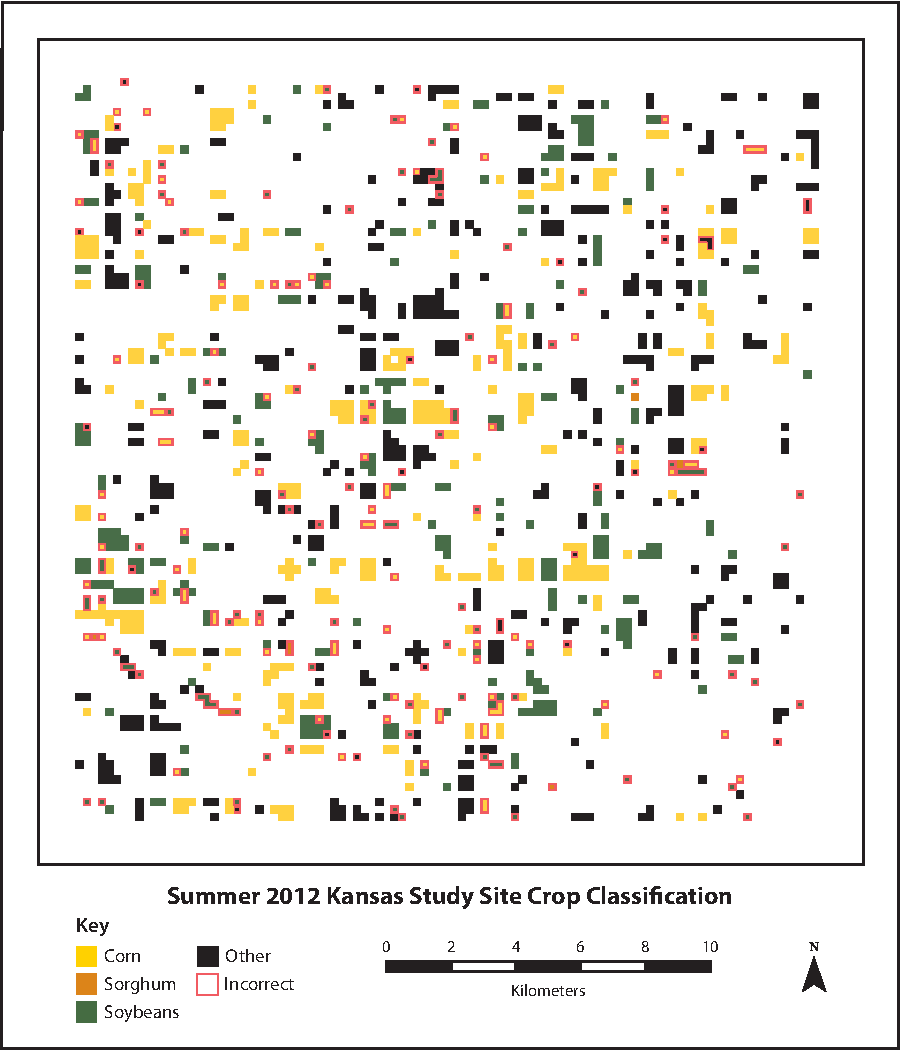
\includegraphics[width=0.55\textwidth]{Graphics/KSclass.pdf}
  %\caption[]{Kansas Summer 2012 Classification}
  %These are the results of classifying the summer 2012 Kansas TSI using corn, soy, and sorghum signatures. Incorrectly classified pixels are shown outlined in red. Omitted mixels were not symbolized, and appear white like the background.
\end{figure}
\end{frame}

\begin{frame}{Kansas Verification Classification}
\begin{table}
  \scriptsize
  \centering
  \caption{Summer 2012 Kansas Classification Accuracy}
  \begin{tabular}{rrrrrrrl}
    \toprule
    & & \multicolumn{4}{c}{\textbf{Reference Data}} & & \\
     &  & Corn & Soy & Sorghum & Other & Total & User Acc. \\
    \midrule
    \multirow{4}{*}{\rotatebox{90}{\textbf{Classified}}} & Corn & 369 & 65 & 5 & 17 & 456 & 80.92\% \\
     & Soy & 32 & 273 & 10 & 47 & 362 & 75.41\% \\
     & Sorghum & 0 & 0 & 2 & 6 & 8 & 25.00\% \\
     & Other & 13 & 16 & 1 & 503 & 533 & 94.37\% \\
    \addlinespace
     & Total & 414 & 354 & 18 & 573 & 1359 &  \\
    \addlinespace
    \multicolumn{2}{r}{Producer Acc.} & 89.13\% & 77.12\% & 11.11\% & 87.78\% &  &  \\
    \addlinespace
    \multicolumn{8}{r}{Overall Accuracy: 84.40\%} \\
    \multicolumn{8}{r}{Kappa: 0.76} \\
    \bottomrule
  \end{tabular}
\end{table}
\end{frame}

\begin{frame}{Kansas Verification Classification}
\begin{table}
  \centering
  \caption{\parbox{2in}{\centering~Kansas Classification RMSE Thresholds}}
  \begin{tabular}{lr}
    \toprule
    \Book{Signature} & \Book{Threshold Value} \\
    \midrule
    Corn\_1 & 1000 \\
    Corn\_2 & 750 \\
    \action<1-|alert@2>{Corn\_3} & \action<1-|alert@2>{500} \\
    Soy\_1 & 750 \\
    Soy\_2 & 1300 \\
    \action<1-|alert@2>{Soy\_3} & \action<1-|alert@2>{500} \\
    \action<1-|alert@2>{Sorghum} & \action<1-|alert@2>{450} \\
    \bottomrule
  \end{tabular}
\end{table}
\end{frame}


\subsection{Pellegrini Classification}
\begin{frame}{Pellegrini Classification}
\begin{table}
  \scriptsize
  \centering
  \caption{Summer 2014 Pellegrini Classification Accuracy}
  \begin{tabular}{rrrrrrrl}
    \toprule
     & & \multicolumn{4}{c}{\textbf{Reference Data}} & & \\
     &  & Corn & Soy & Sorghum & Other & Total & User Acc. \\
    \midrule
    \multirow{4}{*}{\rotatebox{90}{\textbf{Classified}}} & Corn & 24 & 13 & 0 & 8 & 45 & 53.33\% \\
     & Soy & 0 & 2 & 1 & 2 & 5 & 40.00\% \\
     & Sorghum & 0 & 0 & 0 & 0 & 0 & 0.00\% \\
     & Other & 12 & 9 & 1 & 306 & 328 & 93.29\% \\
    \addlinespace
     & Total & 36 & 24 & 2 & 316 & 378 &  \\
    \addlinespace
    \multicolumn{2}{r}{Producer Acc.} & 66.67\% & 8.33\% & 0.00\% & 96.84\% &  &  \\
    \addlinespace
    \multicolumn{8}{r}{Overall Accuracy: 87.83\%} \\
    \multicolumn{8}{r}{Kappa: 0.54} \\
    \bottomrule
  \end{tabular}
\end{table}
\end{frame}

\begin{frame}{Pellegrini Classification}
\begin{table}
  \centering
  \caption{\parbox{4in}{\centering~Pellegrini Best Classification\\RMSE Thresholds}}
  \begin{tabular}{lr}
    \toprule
    \Book{Signature} & \Book{Threshold Value} \\
    \midrule
    Corn\_1 & 550 \\
    Corn\_2 & 850 \\
    \action<1-|alert@2>{Corn\_3} & \action<1-|alert@2>{0} \\
    \action<1-|alert@2>{Soy\_1} & \action<1-|alert@2>{0} \\
    Soy\_2 & 600 \\
    Soy\_3 & 950 \\
    \action<1-|alert@2>{Sorghum\_1} & \action<1-|alert@2>{0} \\
    \bottomrule
  \end{tabular}
\end{table}
\end{frame}

\begin{frame}{Pellegrini Classification}
\begin{figure}
  \centering
  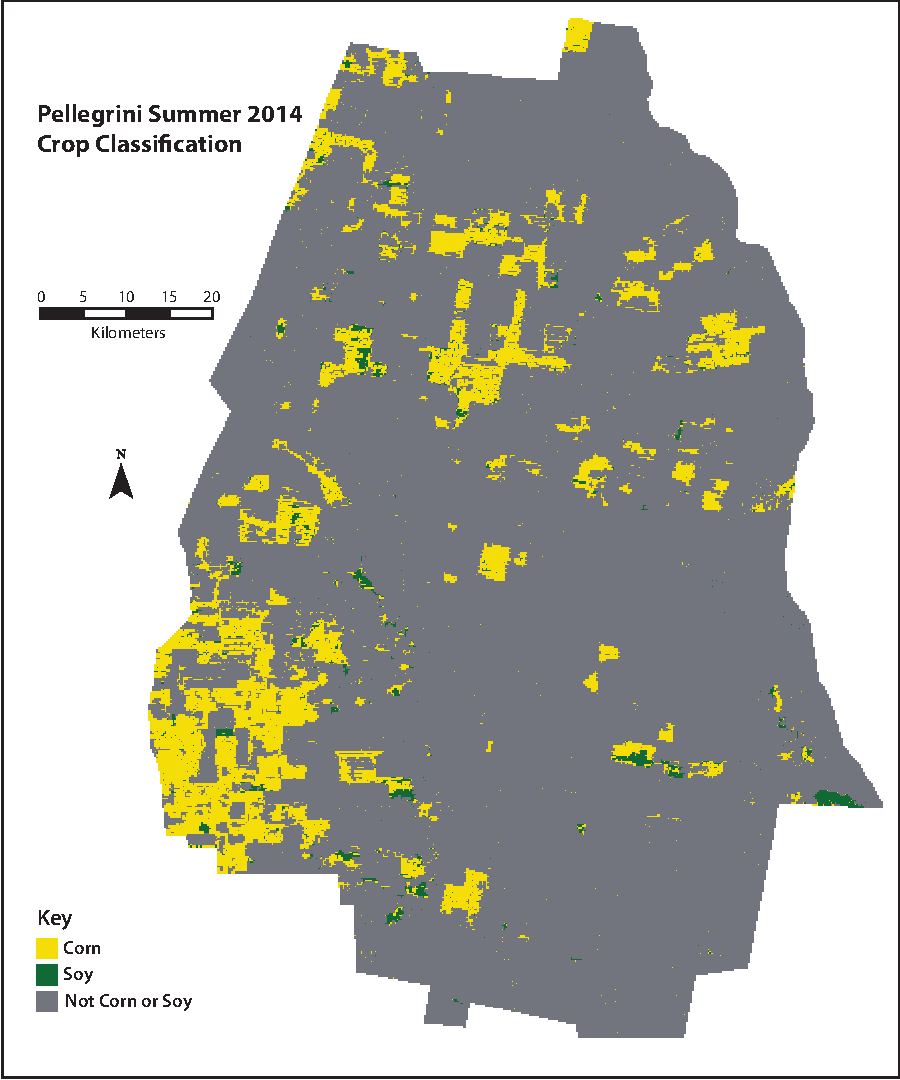
\includegraphics[width=0.53\textwidth]{Graphics/ARclassed.pdf}
  %\caption[Pellegrini Summer 2014 Classification]{Pellegrini Summer 2014 Classification}
  %Comparing this map to the ground truth in \cref{map:pellegrini:groundtruth} on \cpageref{map:pellegrini:groundtruth}, one can see how well the classification was able to separate soy and corn fields from the other classes. However, those fields are overwhelmingly classified as corn, suggesting major class confusion between the two. 
\end{figure}
\end{frame}

\begin{frame}{Pellegrini Classification}
\begin{table}
  \scriptsize
  \centering
  \caption{Pellegrini Classification Checked Against All Pure Pixels}
  \begin{tabular}{rrrrrrrl}
    \toprule
     & & \multicolumn{4}{c}{\textbf{Reference Data}} & & \\
     &  & Corn & Soy & Sorghum & Other & Total & User Acc. \\
    \midrule
    \multirow{4}{*}{\rotatebox{90}{\textbf{Classified}}} & Corn & 3283 & 2076 & 61 & 1201 & 6621 & 49.58\% \\
     & Soy & 189 & 313 & 36 & 458 & 996 & 31.43\% \\
     & Sorghum & 0 & 0 & 0 & 0 & 0 & 0.00\% \\
     & Other & 2234 & 1523 & 60 & 74387 & 78204 & 95.12\% \\
    \addlinespace
     & Total & 5706 & 3912 & 157 & 76046 & 85821 &  \\
    \addlinespace
    \multicolumn{2}{r}{Producer Acc.} & 57.54\% & 8.00\% & 0.00\% & 97.82\% &  &  \\
    \addlinespace
    \multicolumn{8}{r}{Overall Accuracy: 90.87\%} \\
    \multicolumn{8}{r}{Kappa: 0.51} \\
    \bottomrule
  \end{tabular}
\end{table}
\end{frame}

\begin{frame}{Pellegrini Classification}
\begin{table}
  \scriptsize
  \centering
  \caption{\parbox{4in}{\small\centering~Pellegrini Corn and Soy Confusion with\\Other Land Cover Classes}}
  \begin{tabular}{lSSS[table-figures-decimal=2]SS[table-figures-decimal=2]}
    \toprule
    \multirow{2}{*}{\textbf{Land Cover}} & \multirow{2}{*}{\parbox{0.35in}{\raggedleft\textbf{Total Pixels}}} & \multirow{2}{*}{\parbox{0.53in}{\raggedleft\textbf{Confused as Corn}}} & \multirow{2}{*}{\parbox{0.5in}{\raggedleft\textbf{Percent of Total}}} & \multirow{2}{*}{\parbox{0.53in}{\raggedleft\textbf{Confused as Soy}}} & \multirow{2}{*}{\parbox{0.5in}{\raggedleft\textbf{Percent of Total}}} \\
     & & & & \\
    \midrule
    Forested & 63978 & 194 & 0.30 & 26 & 0.04 \\
    Other & 5393 & 306 & 5.67 & 322 & 5.97 \\
    Pasture & 5252 & 396 & 7.54 & 50 & 0.95 \\
    Poroto & 1369 & 303 & 22.13 & 59 & 4.31 \\
    Nothing & 485 & 2 & 0.41 & 1 & 0.21 \\
    \bottomrule
  \end{tabular}
\end{table}
\end{frame}


% CONCLUSION
\section{Conclusion}



% APPENDIX
\appendix

\begingroup
  \setbeamercolor{background canvas}{bg=hsrmWarmGreyDark}
  \begin{frame}[plain]
    \AddToShipoutPictureFG*{
\includegraphics[width=\paperwidth]{background2.pdf}}
    \centering
    \vfill\usebeamerfont{section title}\textcolor{white}{\MakeUppercase{Appendix}}
    \vfill
  \end{frame}
\endgroup
  
\section*{Appendix}

\begin{frame}{Appendix Contents}
  \tableofcontents
\end{frame}

\section{Pellegrini Fieldwork}
\begin{frame}{Pellegrini Fieldwork}
\end{frame}

\section{TSI Processing Toolset}
\begin{frame}{TSI Processing Toolset}
Python tools with command line interfaces:
\begin{itemize}
  \item Build Multidate Image Tool
  \item Extract Signatures Tool
  \item Find Fit Tool
  \item Classify Tool
  \item Other python and command line utilities\\(plotting, masking, etc.)
\end{itemize}
\end{frame}
 

\section{Initial Testing}
\begin{frame}{Initial Testing sites}
\begin{figure}
  \centering
  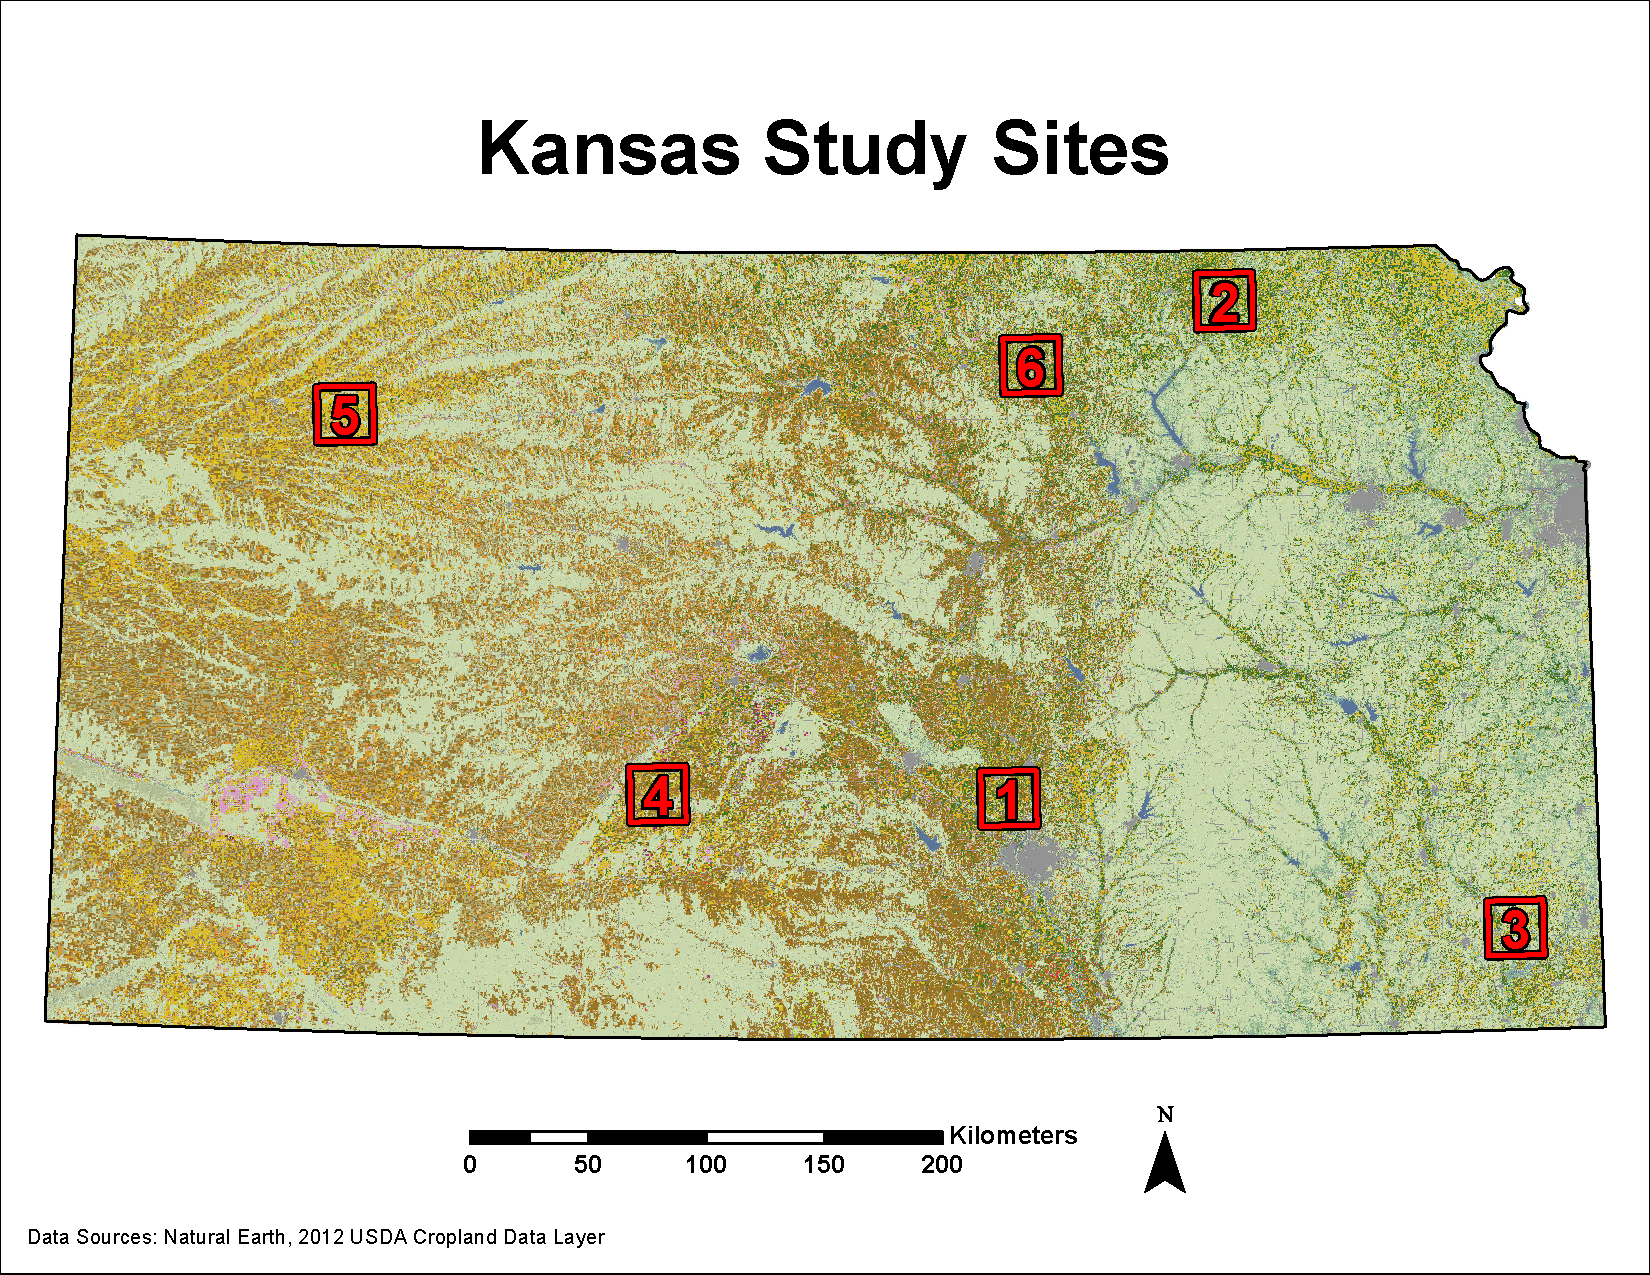
\includegraphics[width=0.85\textwidth]{Graphics/Testing/STUDYSITES.pdf}
\end{figure}
\end{frame}

\begin{frame}{Initial Testing Questions}
How is classification accuracy affected by:
\begin{itemize}
  \item The spatial distribution of pixels chosen to create the reference curves.
  \item The temporal distribution of pixels chosen to create the reference curves.
  \item The VI used for the classification.
\end{itemize}
\end{frame}

\begin{frame}{Initial Testing Procedure}
\begin{itemize}
  \item Built TSIs with NDVI and Enhanced VI (EVI) data
  \item Covered DOY 17 of 2012 to DOY 1 of 2013
  \item Sampled crop pixels in center of fields
  \begin{itemize}
    \item Tried to get at least 5 points per crop per site
  \end{itemize}
\end{itemize}
\end{frame}

\subsection{Round 1 Testing}
\begin{frame}{Round 1 Testing -- Possible Results}
\begin{enumerate}
  \item Reference signatures are usable between study sites, but averaging multiple sites increases classification accuracy.
%  Classification accuracies will be largely independent of the reference signature set used. However, the mean reference signatures will produce a higher classification accuracy than those derived from single study sites.
  \item Reference signatures are usable between study sites, but averaging multiple sites decreases classification accuracy.
%  Classification accuracies will be largely independent of the reference signature set used. However, the mean reference signatures will produce a lower classification accuracy than those derived from single study sites.
  \item Reference signatures are not useable between study sites.
%  Classifications using reference signatures from different study sites will have consistently lower accuracies than the study site's own reference signatures. The mean reference signatures will perform somewhere between those of the study site in question and those of the other study sites.
  \item Spatial distribution has no effect.
%  The classification accuracies will be relatively consistent no matter which reference signature set is used.
\end{enumerate}
\end{frame}

\begin{frame}{Round 1 Testing -- Accuracies}
\begin{table}
  \scriptsize
  \centering
  \caption{Overall Accuracy of Round 1 Classifications}
  \begin{tabular}{lrrrrrrr}
    \toprule
    \Book{EVI} & \multicolumn{7}{c}{Reference Signatures Source} \\
    & SS 1 & SS 2 & SS 3 & SS 4 & SS 5 & SS 6 & Mean \\
    \midrule
    SS 1 & \cellcolor{LimeGreen}55.61 & & 45.34 & 54.36 & 43.83 & 49.06 & 49.63\\
    \rowcolor{light-gray}SS 2 & 53.11 & \cellcolor{LimeGreen}64.93 & 50.00 & 47.86 & 40.79 & 42.60 & 53.69 \\
    SS 3 & 73.87 & 69.40 & \cellcolor{LimeGreen}75.23 & 73.53 & 70.57 & 71.86 & 73.71 \\
    \rowcolor{light-gray}SS 4 & 50.42 & 45.54 & 49.26 & \cellcolor{LimeGreen}53.46 & 45.30 & 49.66 & 52.54 \\
    SS 5 & 42.05 & 45.62 & \cellcolor{LimeGreen}56.00 & 54.68 & 55.06 & 49.02 & 40.29 \\
    \rowcolor{light-gray}SS 6 & 47.78 & 48.66 & 38.43 & 47.53 & 41.60 & \cellcolor{LimeGreen}49.55 & 48.44 \\
    \bottomrule
  \end{tabular}
  \vspace{\baselineskip}
  \begin{tabular}{lrrrrrrr}
    \toprule
    \Book{NDVI} & \multicolumn{7}{c}{Reference Signatures Source} \\
    & SS 1 & SS 2 & SS 3 & SS 4 & SS 5 & SS 6 & Mean \\
    \midrule
    SS 1 & \cellcolor{LimeGreen}61.08 & 48.29 & 47.91 & 60.72 & 44.85 & 51.81 & 52.75 \\
    \rowcolor{light-gray}SS 2 & 56.08 & \cellcolor{LimeGreen}67.39 & 42.66 & 52.59 & 50.62 & 48.95 & 61.21 \\
    SS 3 & 74.88 & 71.75 & \cellcolor{LimeGreen}78.69 & 77.16 & 70.62 & 71.75 & 73.70 \\
    \rowcolor{light-gray}SS 4 & 56.30 & 42.25 & 46.89 & \cellcolor{LimeGreen}59.21 & 44.72 & 54.26 & 52.48 \\
    SS 5 & 53.57 & 48.51 & 45.93 & 62.18 & \cellcolor{LimeGreen}62.83 & 60.21 & 53.07 \\
    \rowcolor{light-gray}SS 6 & & 51.90 & 38.28 & 49.82 & 47.15 & \cellcolor{LimeGreen}55.71 & 54.36 \\
    \bottomrule
  \end{tabular}
\end{table}
\end{frame}


\subsection{Weird Crop Signatures}
\begin{frame}{Weird Crop Signatures}
Hahahahah
\end{frame}





\end{document}






